\باب{اعدادی تراکیب برائے تفرقی مساوات}

\حصہ{یک درجی تفرقی مساوات کے اعدادی تراکیب}
ہم باب \حوالہ{باب_سادہ_اول_تفرقی} سے جانتے ہیں کہ \عددی{F(x,y,y')=0} جس کو عموماً \عددی{y'=f(x,y)} لکھنا ممکن ہو گا، یک درجی تفرقی مساوات ہے۔\اصطلاح{ابتدائی قیمت مسئلہ}\فرہنگ{ابتدائی!قیمت مسئلہ}\حاشیہب{initial value problem}\فرہنگ{initial!value problem} سے مراد ایک تفرقی مساوات اور ایک ایسی شرط ہے  جس کو (بلند درجی تفرقی مسئلے کی صورت میں ایک ہی \عددی{x} پر ایسی کئی شرائط ہوں گے جنہیں) تفرقی مساوات کا حل مطمئن کرتا ہو۔اس حصہ میں ہم درج ذیل روپ کی ابتدائی قیمت مسئلہ پر غور کرتے ہیں
\begin{align}\label{مساوات_اعدادی_ابتدائی_مسئلہ_الف}
y'=f(x,y),\quad y(x_0)=y_0
\end{align}
جہاں ہم فرض کرتے ہیں کہ کسی وقفہ جس پر \عددی{x_0} پایا جاتا ہو میں \عددی{f} کا یکتا حل موجود ہے۔ہم اس ابتدائی مسئلے کے حل کی اعدادی تراکیب تلاش کرتے ہیں۔

اگر ہم اس مسئلے کے حل کا کلیہ اخذ کر سکیں تب کلیہ سے اعدادی جوابات حاصل کیے جا سکتے ہیں۔اگر حل کا کلیہ بہت پیچیدہ ہو یا ایسا کلیہ موجود ہی نہ ہو تب ہم اس حصے کے  اعدادی تراکیب استعمال کر سکتے ہیں۔

یہ تراکیب \اصطلاح{قدم با قدم تراکیب}\فرہنگ{قدم با قدم ترکیب}\حاشیہب{step by step method}\فرہنگ{step by step method} ہیں جن میں ہم  \عددی{y_0=y(x_0)} سے شروع کرتے ہوئے قدم با قدم آگے بڑھتے ہیں۔پہلی قدم پر ہم  \عددی{x=x_1=x_0+h} پر مساوات \حوالہ{مساوات_اعدادی_ابتدائی_مسئلہ_الف} کے حل \عددی{y} کا تخمینہ \عددی{y_1} حاصل کرتے ہیں۔دوسری قدم پر ہم  \عددی{x=x_2=x_0+2h} پر اس حل کا تخمینہ \عددی{y_2} حاصل کرتے ہیں، وغیرہ وغیرہ۔یہاں \عددی{h} ایک مقررہ مستقل ہے مثلاً \عددی{0.2} یا \عددی{0.1} اور یا \عددی{0.01}؛ مستقل \عددی{h} منتخب کرنے کی اصول پر اسی حصے میں غور کیا جائے گا۔

ہر قدم پر ایک ہی جیسی (کلیات) حساب دہرائی جاتی ہے۔ان کلیات کو ٹیلر تسلسل
\begin{align*}
y(x+h)=y(x)+hy'(x)+\frac{h^2}{2}y''(x)+\cdots
\end{align*}
 سے اخذ کیا جا سکتا ہے۔ مساوات \حوالہ{مساوات_اعدادی_ابتدائی_مسئلہ_الف} سے \عددی{y'=f} حاصل ہوتا ہے جس  کا تفرق
\begin{align*}
y''=f'=\tfrac{\partial f}{\partial x}+\tfrac{\partial f}{\partial y}y'
\end{align*}
دیتا ہے۔اسی طرح بلند درجی تفرق کے کلیات اخذ کیے جا سکتے ہیں۔یوں ٹیلر تسلسل کو
\begin{align}\label{مساوات_اعدادی_ابتدائی_مسئلہ_ب}
y(x+h)=y(x)+hf+\frac{h^2}{2}f'+\frac{h^3}{6}f''+\cdots
\end{align}
لکھا جا سکتا ہے جہاں \عددی{f}، \عددی{f'}،\عددی{f''}،\نقطے کی قیمتیں \عددی{(x,y(x))} پر  لی جائیں گی۔\عددی{h} کی چھوٹی قیمتوں کے لئے \عددی{h^2}، \عددی{h^3}، \نقطے قابل نظر انداز ہوں گے۔یوں مساوات \حوالہ{مساوات_اعدادی_ابتدائی_مسئلہ_ب} درج ذیل صورت اختیار کرتی ہے۔
\begin{align*}
y(x+h)\approx y(x)+hf
\end{align*}
پہلی قدم میں ہم 
\begin{align*}
y_1=y_0+h(x_0,y_0)
\end{align*}
کا حساب کرتے ہیں جو \عددی{y(x_1)=y(x_0+h)} کا تخمینہ ہو گا۔دوسری قدم میں ہم
 \begin{align*}
y_2=y_1+h(x_1,y_1)
\end{align*}
کا حساب کرتے ہیں جو \عددی{y(x_2)=y(x_0+2h)} کا تخمینہ ہو گا۔اسی طرح قدم با قدم چلتے ہوئے تمام تخمینی قیمتیں حاصل کی جاتی ہیں۔کسی بھی قدم کی عمومی مساوات
\begin{align}\label{مساوات_اعدادی_ابتدائی_مسئلہ_پ}
y_{n+1}=y_n+hf(x_n,y_n)\quad\quad\quad (n=0,1,\cdots)
\end{align}
ہو گی۔اس قدم با قدم ترکیب کو \اصطلاح{ترکیب یولر}\فرہنگ{ترکیب یولر}\حاشیہب{Euler method}\فرہنگ{Euler!method} یا \اصطلاح{یولر کوشی ترکیب}\فرہنگ{یولر کوشی ترکیب}\حاشیہب{Euler-Cauchy method}\فرہنگ{Euler Cauchy method} کہتے ہیں۔ جیومیٹریائی طور پر اس ترکیب میں  منحنی \عددی{y(x)} کی جگہ اس کی ایسی تخمینی کثیر الاضلاع استعمال کی جاتی ہے جس کا پہلا بازو نقطہ \عددی{x_0} پر منحنی کا مماس ہو (شکل \حوالہ{شکل_اعدادی_ترکیب-یولر})۔
\begin{figure}
\centering
\begin{tikzpicture}
\draw[stealth-stealth] (3,0.25)--++(1,0)node[pos=0.5,fill=white]{$h$};
\draw[stealth-stealth] (4,0.25)--++(1,0)node[pos=0.5,fill=white]{$h$};
\draw(0,0)--(6,0)node[right]{$x$};
\draw(0,0)--(0,2.5)node[left]{$y$};
\draw(3,1) to [out=7.5,in=-135] ++(3,1.5);
\draw(3,1)coordinate(kA)--++(1,0.1)coordinate(kB)--++(1,0.4)coordinate(kC);
\draw(kA)node[ocirc]{}--($(0,0)!(kA)!(4,0)$)node[below]{$x_0$}node[pos=0.5,left]{$y_0$};
\draw(kB)node[ocirc]{}--($(0,0)!(kB)!(4,0)$)node[below]{$x_1$}node[pos=0.35,right]{$y_1$};
\draw(kC)node[ocirc]{}--($(0,0)!(kC)!(4,0)$)node[below]{$x_2$}node[pos=0.5,right]{$y_2$};
\draw[stealth-]($(kA)!0.75!(kB)$)node[]{} to [out=-120,in=0]++(-1.25,-0.25)node[left]{$f(x_0,y_0)\,\text{ڈھلوان}$};
\draw[stealth-]($(kB)!0.75!(kC)$)node[]{} to [out=-60,in=180]++(0.75,-0.25)node[right]{$f(x_1,y_1)\,\text{ڈھلوان}$};
\end{tikzpicture}
\caption{ترکیب یولر}
\label{شکل_اعدادی_ترکیب-یولر}
\end{figure}

مساوات \حوالہ{مساوات_اعدادی_ابتدائی_مسئلہ_ب} میں مستقل کے علاوہ اکائی طاقت کا  \عددی{h}  لے کر ترکیب یولر حاصل کی گئی  لہٰذا ترکیب یولر  کو \اصطلاح{درجہ اول ترکیب}\فرہنگ{ترکیب!درجی اول}\حاشیہب{first order method}\فرہنگ{method!first order} کہتے ہیں۔مساوات \حوالہ{مساوات_اعدادی_ابتدائی_مسئلہ_ب} کے باقی اجزاء کو رد کرنے کی وجہ سے حل میں خلل پیدا ہوتا ہے جس کو  اس ترکیب کی \اصطلاح{حذفی خلل}\فرہنگ{خلل!قطع چال}\فرہنگ{error!truncation} کہتے ہیں۔\عددی{h} کی چھوتی قیمت کی صورت میں \عددی{h^3}، \عددی{h^4}، وغیرہ کی قیمت \عددی{h^2} کی قیمت سے بہت کم ہوں گی لہٰذا ہم کہہ سکتے ہیں کہ \اصطلاح{فی قدم حذفی خلل} کا \اصطلاح{درجہ} \عددی{h^2} ہے۔ اس کے علاوہ  اس ترکیب میں اور دیگر تراکیب میں \اصطلاح{پور و پور خلل} بھی پائے جائیں گے جن کی بنا \عددی{n} بڑھانے سے  \عددی{y_1}،\عددی{y_2}،\نقطے کی قیمتوں میں خلل بتدریج بڑھتا جائے گا۔اس حقیقت پر اگلے حصے میں غور کیا جائے گا۔

%=========================
\ابتدا{مثال}\شناخت{مثال_اعدادی_ترکیب_یولر_الف}\quad \موٹا{ترکیب یولر}\\
ترکیب یولر سے درج ذیل ابتدائی قیمت مسئلہ حل کریں۔
\begin{align*}
y'=x+y,\quad y(0)=0
\end{align*}
حل:\quad
ہم \عددی{h=0.2} منتخب کرتے ہوئے \عددی{y_1} تا  \عددی{y_5} حاصل کرتے ہیں۔یہاں \عددی{f(x,y)=x+y} ہے لہٰذا مساوات \حوالہ{مساوات_اعدادی_ابتدائی_مسئلہ_پ} درج ذیل روپ اختیار کرتی ہے۔
\begin{align*}
y_{n+1}=y_n+0.2(x_n,y_n)
\end{align*}
جدول \حوالہ{جدول_مثال_اعدادی_ترکیب_یولر_الف} میں ترکیب یولر سے حاصل نتائج کے ساتھ ساتھ مساوات \حوالہ{مساوات_سادہ_اول_متجانس_خطی_حل_الف} سے حاصل بالکل درست حل
\begin{align*}
y(x)=e^x-x-1
\end{align*}
کی قیمتیں اور خلل بھی دی گئی ہیں۔موجودہ مثال میں ہمیں اصل حل بھی معلوم ہے لہٰذا ہم ترکیب یولر کی درستگی کا مطالعہ کر سکتے ہیں۔\عددی{h} کی مختلف قیمتیں لے کر آپ ترکیب یولر سے حاصل نتائج کا اصل حل کے ساتھ موازنہ کر سکتے ہیں۔
\begin{table}
\caption{جدول برائے مثال \حوالہ{مثال_اعدادی_ترکیب_یولر_الف}}
\label{جدول_مثال_اعدادی_ترکیب_یولر_الف}
\centering
\begin{otherlanguage}{english}
\begin{tabular}{C|C|C|C|C|C}
\hline
n&x_n&y_n&0.2(x_n+y_n)&\text{\RL{\urdufont{درست حل}}}&\text{\RL{\urdufont{مطلق خلل}}}\\
\hline
0&0.0&0.000&0.000&0.000&0.000\\
1&0.1&0.000&0.040&0.021&0.021\\
2&0.2&0.040&0.088&0.092&0.052\\
3&0.3&0.128&0.146&0.222&0.094\\
4&0.4&0.274&0.215&0.426&0.152\\
5&0.5&0.489&&0.718&0.229\\
\hline
\end{tabular}
\end{otherlanguage}
\end{table}
\انتہا{مثال}
%=============================

مساوات \حوالہ{مساوات_اعدادی_ابتدائی_مسئلہ_ب} کے زیادہ اجزاء شامل کرتے ہوئے بہتر اعدادی تراکیب حاصل کیے جا سکتے ہیں۔ایسے کلیات میں عموماً \عددی{f(x,y)} کی تفرق سے چھٹکارا حاصل کرنے کی خاطر تفرق   کو دیگر موزوں نقطوں پر \عددی{f(x,y)} کی قیمتوں سے حاصل کیا جاتا  ہے۔آئیں ایسی دو تراکیب پر غور کرتے ہیں۔

ایسی پہلی ترکیب کو \اصطلاح{بہتر ترکیب یولر}\فرہنگ{یولر!بہتر ترکیب}\حاشیہب{improved Euler method}\فرہنگ{Euler!improved method} یا \موٹا{یولر کوشی کی بہتر  ترکیب} کہتے ہیں۔اس ترکیب کی پہلی قدم میں ہم پہلے ذیلی قیمت
\begin{align}\label{مساوات_اعدادی_بہتر_یولر_الف}
y^*_{n+1}=y_n+hf(x_n,y_n)
\end{align}
اور بعد میں نئی قیمت
\begin{align}\label{مساوات_اعدادی_بہتر_یولر_ب}
y_{n+1}=y_n+\frac{h}{2}[f(x_n,y_n)+f(x_{n+1},y^*_{n+1})]
\end{align}
حاصل کرتے ہیں۔
\begin{figure}
\centering
\begin{tikzpicture}
\draw[stealth-stealth] (1,0.4)--++(1,0)node[pos=0.5,fill=white]{$\frac{h}{2}$};
\draw[stealth-stealth] (2,0.4)--++(1,0)node[pos=0.5,fill=white]{$\frac{h}{2}$};
\draw(0,0)--(4,0)node[right]{$x$};
\draw(0,0)--(0,2.5)node[left]{$y$};
\draw(1,1) to [out=7.5,in=-135] ++(3,1.5);
\draw(1,1)coordinate(kA)--++(1,0.1)coordinate(kB)--++(1,0.4)coordinate(kC);
\draw(kA)node[ocirc]{}--($(0,0)!(kA)!(4,0)$)node[below]{$x_0$}node[pos=0.5,left]{$y_0$};
\draw(kB)--($(0,0)!(kB)!(4,0)$);
\draw(kC)--($(0,0)!(kC)!(4,0)$)node[below]{$x_1$};
\end{tikzpicture}
\caption{بہتر ترکیب یولر}
\label{شکل_اعدادی_بہتر_ترکیب-یولر}
\end{figure}

یہ ترکیب ایک سادہ جیومیٹریائی مطلب رکھتی ہے۔ ہم کہہ سکتے ہیں کہ وقفہ \عددی{x_n} تا \عددی{x_n+\tfrac{1}{2}h} تک ہم حل کو تخمیناً ایسی قطع سے ظاہر کرتے ہیں جو نقطہ \عددی{(x_n,y_n)} سے گزرتی ہو اور جس کی ڈھلوان \عددی{f(x_n,y_n)} ہو جبکہ باقی وقفہ، یعنی  \عددی{x_n+\tfrac{1}{2}h} تا \عددی{x_n} تک، ہم قطع کی ڈھلوان \عددی{f(x_{n+1},y^*_{n+1})} لیتے ہیں (شکل \حوالہ{شکل_اعدادی_بہتر_ترکیب-یولر} جہاں \عددی{n=0} ہے)۔ 

بہتر ترکیب یولر کے ہر قدم پر پہلے  مساوات \حوالہ{مساوات_اعدادی_بہتر_یولر_الف} سے قیمت کی پیش گوئی کی جاتی ہے اور بعد میں مساوات \حوالہ{مساوات_اعدادی_بہتر_یولر_ب}  سے قیمت کی  تصحیح کی جاتی ہے لہٰذا یہ  \اصطلاح{پیش گو، مصحح ترکیب}\فرہنگ{پیش گو، مصحح ترکیب}\حاشیہب{predictor-corrector method}\فرہنگ{predictor-corrector method} کہلاتی ہے۔

%==================
\ابتدا{مثال}\شناخت{مثال_اعدادی_بہتر_ترکیب_یولر_الف}\quad \موٹا{بہتر ترکیب یولر}\\
پہلے کی طرح \عددی{h=0.2} لیتے ہوئے بہتر ترکیب یولر کو مثال \حوالہ{مثال_اعدادی_ترکیب_یولر_الف} کی ابتدائی قیمت مسئلے پر لاگو کریں۔یہاں مساوات \حوالہ{مساوات_اعدادی_بہتر_یولر_الف} اور مساوات \حوالہ{مساوات_اعدادی_بہتر_یولر_ب} درج ذیل ہوں گی۔
\begin{align*}
y^*_{n+1}&=y_n+0.2(x_n+y_n)\\
y_{n+1}&=y_n+0.1[(x_n+y_n)+(x_{n+1}+y^*_{n+1})]
\end{align*}
پہلی مساوات کو دوسری مساوات میں پر کرتے ہوئے ایک ہی قدم میں دو بار حساب کی بجائے ایک بار حساب کرنا ہو گا۔یوں درج ذیل حاصل ہو گا۔
\begin{align*}
y_{n+1}=0.12x_n+0.1x_{n+1}+1.22y_n
\end{align*}
ہم جدول \حوالہ{جدول_مثال_اعدادی_بہتر_ترکیب_یولر_الف} سے دیکھتے ہیں کہ موجودہ نتائج مثال \حوالہ{مثال_اعدادی_ترکیب_یولر_الف} میں حاصل کردہ نتائج سے بہتر ہیں۔
\begin{table}
\caption{بہتر ترکیب یولر۔ (مثال \حوالہ{مثال_اعدادی_بہتر_ترکیب_یولر_الف})}
\label{جدول_مثال_اعدادی_بہتر_ترکیب_یولر_الف}
\centering
\begin{otherlanguage}{english}
\begin{tabular}{|C|C|C|C|C|C|C|}
\hline
n&x_n&y_n&0.12x_n&0.1x_{n+1}&1.22y_n&y_{n+1}\\
\hline
0&0.0&0.0000&0.0000&0.0200&0.0000&0.0200\\
1&0.2&0.0200&0.0240&0.0400&0.0244&0.0884\\
2&0.4&0.0884&0.0480&0.0600&0.1078&0.2158\\
3&0.6&0.2158&0.0720&0.0800&0.2633&0.4153\\
4&0.8&0.4153&0.0960&0.1000&0.5067&0.7027\\
5&1.0&0.7027&&&&\\
\hline
\end{tabular}
\end{otherlanguage}
\end{table}
\انتہا{مثال}
%======================

بہتر ترکیب یولر میں فی قدم حذفی خلل \عددی{h^3} کے لحاظ سے بڑھتا ہے لہٰذا یہ ترکیب \اصطلاح{درجہ دوم ترکیب}\فرہنگ{درجہ!دوم ترکیب}\حاشیہب{second order method}\فرہنگ{second order method} ہے۔ بلکہ \عددی{\tilde{f}_n=f(x_n,y(x_n))} لکھ کر  مساوات \حوالہ{مساوات_اعدادی_ابتدائی_مسئلہ_ب} استعمال کرنے سے
\begin{align}\label{مساوات_اعدادی_بہتر_یولر_پ}
y(x_n+h)-y_n=h\tilde{f}_n+\frac{1}{2}h^2\tilde{f}_n'+\frac{1}{6}h^3\tilde{f}_n''+\cdots
\end{align}
ملتا ہے۔مساوات \حوالہ{مساوات_اعدادی_بہتر_یولر_ب} میں قوسین میں بند حصہ کو \عددی{\tilde{f}_n+\tilde{f}_{n+1}} لکھ کر دوبارہ ٹیلر تسلسل استعمال کرتے ہوئے مساوات \حوالہ{مساوات_اعدادی_بہتر_یولر_ب} سے  درج ذیل حاصل ہو گا 
\begin{align}\label{مساوات_اعدادی_بہتر_یولر_ت}
y_{n+1}-y_n\approx \frac{1}{2}h(\tilde{f}_n+\tilde{f}_n+h\tilde{f}_n'+\frac{1}{2}h^2\tilde{f}_n''+\cdots)
\end{align}
جس سے مساوات \حوالہ{مساوات_اعدادی_بہتر_یولر_پ} تفریق کرتے ہوئے فی قدم قطع  چال خلل
\begin{align*}
\frac{h^3}{4}\tilde{f}_n''-\frac{h^3}{6}\tilde{f}_n''+\cdots=\frac{h^3}{12}\tilde{f}_n''+\cdots
\end{align*}
حاصل ہو گا۔ 

ہم اب \موٹا{قدم \عددی{h} کی انتخاب} پر غور کرتے ہیں جو قدم با قدم تراکیب استعمال کرنے میں اہم مسئلہ ثابت ہوتا ہے۔\عددی{h} کی قیمت بہت کم رکھنے سے قدموں کی تعداد اور  پور و پور خلل بہت بڑھ جاتے ہیں جبکہ \عددی{h} کی قیمت بہت زیادہ رکھنے سے  فی قدم حذفی خلل بڑھتی ہے اور ساتھ ہی ساتھ ایک اضافی خلل، جو \عددی{f} کی قیمت \عددی{(x_n,y_n)} کی بجائے \عددی{(x_n,y(x_n))} پر حاصل کرنے کی بنا پیدا ہوتا ہے، بھی بڑھتی  ہے۔اگر \عددی{f} متغیر \عددی{y} کے تابع نہ ہو تب ان میں دوسرا خلل صفر کے برابر ہو گا، دیگر حال \عددی{y} کی تبدیلی سے \عددی{f} جتنا زیادہ تبدیل ہو، یہ خلل اتنا زیادہ ہو گا، یعنی \عددی{f_y=\tfrac{\partial f}{\partial y}} کی مطلق قیمت جتنی زیادہ ہو، یہ خلل اتنا زیادہ ہو گا۔بلکہ اس خلل کو \عددی{\varphi_n} سے ظاہر کرتے ہوئے مسئلہ اوسط قیمت کی اطلاق سے 
\begin{align*}
\varphi_n=f(x_n,y_n)-f(x_n,y(x_n))=f_y(x_n,\tilde{y})\eta_n
\end{align*}
حاصل ہو گا جہاں  \عددی{y_n} کا خلل \عددی{\eta_n=y_n-y(x_n)} ہے، اور \عددی{\tilde{y}} کا مقام   \عددی{y_n} اور \عددی{y(x_n)} کے بیچ ہے۔یوں \عددی{y_{n+1}} کے خلل میں \عددی{\varphi_n} کا حصہ تقریباً \عددی{h\varphi_n=hf_y(x_n,\tilde{y}_n)\eta_n} ہو گا۔اس سے ہمیں خیال آتا ہے کہ دلچسپی کے خطہ میں \عددی{\abs{f_y}} کی بالائی حد \عددی{K} کو کم رکھا جائے اور \عددی{h} یوں منتخب کیا جائے کہ
\begin{align*}
\kappa=hK
\end{align*}
بہت زیادہ بڑی قیمت نہ ہو۔ہم دیکھتے ہیں کہ اگر \عددی{\abs{f_y}} کی قیمت زیادہ ہو (جو \عددی{y} پر \عددی{f} کی زیادہ تابعیت کو ظاہر کرتی ہے) تب \عددی{K} بڑا ہو گا لہٰذا ہمیں \عددی{h} چھوٹا رکھنا ہو گا۔ (مثال \حوالہ{مثال_اعدادی_ترکیب_یولر_الف} اور مثال \حوالہ{مثال_اعدادی_بہتر_ترکیب_یولر_الف} میں \عددی{f_y=1}، \عددی{K=1}، \عددی{hK=0.2} ہیں۔) اگر \عددی{f_y} بہت زیادہ تبدیل ہوتا ہو تب ہم \عددی{K} یعنی \عددی{\abs{f_y(x_n,\tilde{y})}} کی بالائی حد کو کم رکھتے ہوئے وقفہ کے مختلف حصوں پر مختلف \عددی{h} منتخب کر سکتے ہیں تا کہ 
\begin{align*}
\kappa_n=hK_n
\end{align*}
کو کسی مخصوص  وقفہ (مثلاً \عددی{0.1\le \kappa_n\le 0.2})، جو  درکار درستگی پر منحصر ہو گا،  میں رکھا جا سکے ۔فی قدم حذفی خلل کی بنا ہم \عددی{h} کو کسی ایک مقررہ  قیمت سے زیادہ نہیں چن سکتے ہیں۔

\جزوحصہء{رنج کوٹا ترکیب}
اس سے بھی زیادہ درست ترکیب جو عملاً انتہائی اہم ہے \اصطلاح{ترکیب رنج کوٹا}\فرہنگ{ترکیب!رنج کوٹا}\فرہنگ{رنج کوٹا ترکیب}\حاشیہب{Runge-Kutta method}\فرہنگ{Runge-Kutta method} کہلاتی\حاشیہد{جرمنی کے ریاضی دان کارل رنج [1856-1927] اور ولہلم کوٹا [1867-1944]} ہے جس کے ہر قدم پر ہم پہلے چار عدد ذیلی قیمتیں
\begin{gather}
\begin{aligned}\label{مساوات_اعدادی_رنج_کوٹا_الف}
A_n&=hf(x_n,y_n),\\
C_n&=hf(x_n+\tfrac{1}{2}h,y_n+\tfrac{1}{2}B_n),
\end{aligned}
\quad 
\begin{aligned}
B_n&=hf(x_n+\tfrac{1}{2}h,y_n+\tfrac{1}{2}A_n),\\
D_n&=hf(x_{n+1},y_n+C_n)
\end{aligned}
\end{gather}
 تلاش کرتے ہیں جنہیں استعمال کرتے ہوئے نئی قیمت
\begin{align}\label{مثال_اعدادی_ترکیب_یولر_ب}
y_{n+1}=y_n+\tfrac{1}{6}(A_n+2B_n+2C_n+D_n)
\end{align}
حاصل کی جاتی ہے۔یہاں ثبوت پیش کیے بغیر بتلاتا چلوں کہ اس ترکیب کی حذفی خلل درجہ \عددی{h^5} ہے یعنی یہ درجہ چار ترکیب  ہے۔دھیان رہے کہ اگر \عددی{f} صرف \عددی{x} کا تابع ہو تب ترکیب رنج کوٹا سے تکمل کی ترکیب سمسن (حصہ \حوالہ{حصہ_اعدادی_اعدادی_تکمل_اور_تفرق}) حاصل ہوتی ہے۔

اگرچہ قلم و کاغذ استعمال کرتے ہوئے ترکیب رنج کوٹا قابل محنت طلب ہے، کمپیوٹر کی استعمال کے لئے یہ ترکیب موزوں ہے۔

%====================
\ابتدا{مثال}\شناخت{مثال_اعدادی_رنج_کوٹا_الف}\quad \موٹا{ترکیب رنج کوٹا}\\
ترکیب رنج کوٹا کو مثال \حوالہ{مثال_اعدادی_ترکیب_یولر_الف} کے ابتدائی قیمت مسئلے پر لاگو کریں۔ہم پہلے کی طرح \عددی{h=0.2} منتخب کرتے ہیں۔یہاں \عددی{f(x,y)=x+y} ہے لہٰذا مساوات \حوالہ{مثال_اعدادی_ترکیب_یولر_الف} درج ذیل صورت اختیار کرتی ہے۔
\begin{gather}
\begin{aligned}
A_n&=0.2(x_n+y_n),\\
C_n&=0.2(x_n+0.1+y_n+0.5B_n),
\end{aligned}
\quad
\begin{aligned}
B_n&=0.2(x_n+0.1+y_n+0.5A_n),\\
D_n&=0.2(x_n+0.2+y_n+C_n)
\end{aligned}
\end{gather}
چونکہ یہ تعلقات سادہ صورت رکھتے ہیں لہٰذا ہم \عددی{A_n} کو \عددی{B_n} میں پر کر کے\عددی{B_n=0.22(x_n+y_n)+0.02} حاصل کرتے ہیں جس کو \عددی{C_n} میں پر کر کے \عددی{C_n=0.222(x_n+y_n)+0.022} حاصل کرتے ہیں جس کو \عددی{D_n} میں پر کر کے \عددی{D_n=0.2444(x_n+y_n)+0.0444} حاصل کرتے ہیں۔ان حاصل کردہ تعلقات کو استعمال کرتے ہوئے  مساوات \حوالہ{مثال_اعدادی_ترکیب_یولر_ب} کو درج ذیل لکھا جا سکتا ہے۔
\begin{align*}
y_{n+1}=y_n+0.2214(x_n+y_n)+0.0214
\end{align*}
جدول\حوالہ{جدول_مثال_اعدادی_رنج_کوٹا_الف} میں حساب دیا گیا ہے۔جدول \حوالہ{جدول_اعدادی_یولر_بہتر_یولر_اور_رنج_کوٹا_موازنہ} میں ترکیب یولر، بہتر ترکیب یولر اور ترکیب رنج کوٹا کے نتائج کا موازنہ کیا گیا ہے جہاں سے آپ دیکھ سکتے ہیں کہ  مثال \حوالہ{مثال_اعدادی_ترکیب_یولر_الف} اور مثال \حوالہ{مثال_اعدادی_بہتر_ترکیب_یولر_الف} کے نتائج سے موجودہ مثال کے نتائج بہت بہتر ہیں۔
\begin{table}
\caption{ترکیب رنج کوٹا (مثال \حوالہ{مثال_اعدادی_رنج_کوٹا_الف})}
\label{جدول_مثال_اعدادی_رنج_کوٹا_الف}
\centering
\begin{otherlanguage}{english}
\begin{tabular}{|C|C|C|C|C|C|}
\hline
n&x_n&y_n&x_n+y_n&0.2214(x_n+y_n)&y_{n+1}\\
\hline
0&0.0&\num{0.000000}&\num{0.000000}&\num{0.000000}&\num{0.021400}\\
1&0.2&\num{0.021400}&\num{0.221400}&\num{0.049018}&\num{0.070418}\\
2&0.4&\num{0.091818}&\num{0.491818}&\num{0.108889}&\num{0.130289}\\
3&0.6&\num{0.222107}&\num{0.822107}&\num{0.182014}&\num{0.203414}\\
4&0.8&\num{0.425521}&\num{1.225521}&\num{0.271330}&\num{0.292730}\\
5&1.0&\num{0.718251}&&&\\
\hline
\end{tabular}
\end{otherlanguage}
\end{table}
%
\begin{table}
\caption{جدول \حوالہ{جدول_مثال_اعدادی_ترکیب_یولر_الف}، جدول \حوالہ{جدول_مثال_اعدادی_بہتر_ترکیب_یولر_الف} اور جدول \حوالہ{جدول_مثال_اعدادی_رنج_کوٹا_الف} میں خلل کا موازنہ}
\label{جدول_اعدادی_یولر_بہتر_یولر_اور_رنج_کوٹا_موازنہ}
\centering
\begin{otherlanguage}{english}
\begin{tabular}{|C|C|C|C|C|}
\hline
\multirow{2}{*}{$x$}&\multirow{2}{*}{$y=e^x-x-1$}&\multicolumn{3}{C|}{\text{\RL{\urdufont{خلل کی مطلق قیمت}}}}\\
\cline{3-5}
&&\text{\RL{\urdufont{ترکیب یولر}}}&\text{\RL{\urdufont{بہتر ترکیب یولر}}}&\text{\RL{\urdufont{ترکیب رنج کوٹا}}}\\
\hline
0.2&\num{0.021403}&\num{0.021}&\num{0.0014}&\num{0.000003}\\
0.4&\num{0.091825}&\num{0.052}&\num{0.0034}&\num{0.000007}\\
0.6&\num{0.222119}&\num{0.094}&\num{0.0063}&\num{0.000011}\\
0.8&\num{0.425541}&\num{0.152}&\num{0.0102}&\num{0.000020}\\
1.0&\num{0.718282}&\num{0.229}&\num{0.0156}&\num{0.000031}\\
\hline
\end{tabular}
\end{otherlanguage}
\end{table}
\انتہا{مثال}
%=====================

\اصطلاح{لمبائی قدم}\فرہنگ{قدم!لمبائی}\حاشیہب{step length}\فرہنگ{step!length} \عددی{h} ایک مخصوص قیمت \عددی{H}، جو درستگی پر منحصر ہے، سے زیادہ نہیں ہونی چاہیے اور اس کی قیمت یوں منتخب کرنی چاہیے کہ
\begin{align*}
\kappa=hK\quad \quad (\text{\RL{\urdufont{\عددی{\abs{\tfrac{\partial f}{\partial y}}} کی بالائی حد \عددی{K} ہے}}})
\end{align*}
کی قیمت \عددی{0.1} اور \عددی{0.2} کے بیچ ہو (جیسا بہتر ترکیب یولر میں تھا)۔ ترکیب رنج کوٹا میں ہم \عددی{h} کو \عددی{A_n}، \عددی{B_n}، \عددی{C_n} سے قابو کر سکتے ہیں چونکہ \عددی{f_y} کی تعریف کی رو سے 
\begin{align*}
\kappa=hK\approx h\abs{f_y}\approx h\abs{\frac{f(x,y^*)-f(x,y^{**})}{y^*-y^{**}}}
\end{align*}
ہو گا اور اگر ہم \عددی{x=x_n+\tfrac{1}{2}h}، \عددی{y^*=y_n+\tfrac{1}{2}B_n}، \عددی{y^{**}=y_n+\tfrac{1}{2}A_n} منتخب کریں تب \عددی{y^*-y^{**}=\tfrac{B_n-A_n}{2}} اور
\begin{align}
\kappa\approx \kappa_n=2\abs{\frac{C_n-B_n}{B_n-A_n}}
\end{align}
ہو گا۔ہم اب کوئی قاعدہ بنا سکتے ہیں مثلاً  جب تک \عددی{0.05\le \kappa_n\le 0.2} ہو ہم \عددی{h} کو  تبدیل نہیں کرتے  جبکہ \عددی{\kappa_n>0.2} کی صورت میں ہم \عددی{h} کو \عددی{\SI{50}{\percent}} کم کرتے ہیں اور \عددی{\kappa_n<0.05} کی صورت میں ہم \عددی{h} کو دگنا کرتے ہیں (اگر \عددی{h} دگنا کرنے سے اس کی قیمت منتخب \عددی{H} سے بڑھتی نہ ہو جہاں \عددی{H} از خود درکار درستگی پر منحصر ہے)۔

\عددی{h} کو قابو کرنے کا دوسرا طریقہ یہ ہے کہ ہم حساب کرنے کے ساتھ ساتھ قدم \عددی{2h} لیتے ہوئے بھی حساب کرتے ہیں جس سے فی قدم حذفی خلل
  \عددی{2^5=32} گنا بڑھتا ہے لیکن قدموں کی تعداد گھٹنے کی بنا اصل خلل \عددی{\tfrac{2^5}{2}=16} گنا بڑھتا ہے۔یوں لمبائی قدم  کو \عددی{h} رکھتے ہوئے خلل کی قیمت مطابقتی \عددی{y} کے فرق  \عددی{\delta} کے تقریباً \عددی{\tfrac{1}{15}} گنا ہو گی۔ ہم اب عدد \عددی{\epsilon} منتخب کرتے ہوئے (مثلاً آخری ہندسے کی اکائی کا نصف، جو بہت بڑی قیمت ہے) \عددی{h} کو اس وقت تک تبدیل نہیں کرتے جب تک \عددی{0.2\epsilon\le \abs{\delta}\le 10\epsilon} ہو، اگر \عددی{\abs{\delta}>10\epsilon} ہو تب ہم \عددی{h} کو \عددی{\SI{50}{\percent}} کم کرتے ہیں اور اگر \عددی{\abs{\delta}<0.2\epsilon} ہو تب ہم \عددی{h} کو دگنا کرتے ہیں؛  ظاہر ہے کہ \عددی{h} کو اس صورت دگنا کرنا ممکن ہو گا جب تک  (پہلے کی طرح) یہ \عددی{H} سے تجاوز نہ کرتا ہو۔

%================
\حصہء{سوالات}
سوال \حوالہ{سوال_اعدادی_یولر_دس_قدم_الف} تا سوال \حوالہ{سوال_اعدادی_یولر_دس_قدم_ب} میں ترکیب یولر استعمال کرتے ہوئے دس قدم تک چلیں۔ 

%====================
\ابتدا{سوال}\شناخت{سوال_اعدادی_یولر_دس_قدم_الف}\quad
$y'=y,\quad y(0)=1,\quad h=0.01$\\
جواب:\quad
$1,1.01,1.0201,1.030301,1.04060401,\cdots$
\انتہا{سوال}
%===========================
\ابتدا{سوال}\quad
$y'=xy,\quad y(1)=1,\quad h=0.1$\\
جواب:\quad
$1,1.1,1.221,1.36752,1.5452976,\cdots$
\انتہا{سوال}
%===========================
\ابتدا{سوال}\quad
$y'=xy-1,\quad y(0)=0,\quad h=0.1$\\
جواب:\quad
$0,-0.1,-0.201,-0.30502,\cdots$
\انتہا{سوال}
%===========================
\ابتدا{سوال}\شناخت{سوال_اعدادی_یولر_دس_قدم_ب}\quad
$y'=xy,\quad y(0)=1,\quad h=0.1$\\
جواب:\quad
$1,1,1.01,1.0302,1.061106,\cdots$
\انتہا{سوال}
%===========================
\ابتدا{سوال}\quad
$y'=2x,\quad y(0)=0,\quad h=0.1$
کو بہتر ترکیب یولر سے حل کریں۔خلل صفر کے برابر کیوں ہے؟\\
جواب:\quad
$0,0.01,0.04,0.09,0.16,\cdots$
\انتہا{سوال}
%====================== 
\ابتدا{سوال}\quad
ایسی چند مثالیں پیش کریں جہاں بہتر ترکیب یولر بالکل درست جواب دیتی ہو۔
\انتہا{سوال}
%==========================
\ابتدا{سوال}\quad
\عددی{h=0.1} لیتے ہوئے مثال \حوالہ{مثال_اعدادی_ترکیب_یولر_الف} کو دوبارہ حل کریں۔آپ دیکھیں گے کہ خلل مثال \حوالہ{مثال_اعدادی_ترکیب_یولر_الف} کے خلل کا \عددی{\SI{50}{\percent}} ہو گا۔\\
جواب:\quad
$0,0,0.01,0.031,0.0641,0.11051,0.171561,\cdots$
\انتہا{سوال}
%==========================
\ابتدا{سوال}\quad
\عددی{h=0.01} (بیس قدم) لیتے ہوئے مثال \حوالہ{مثال_اعدادی_ترکیب_یولر_الف} کو دوبارہ حل کریں۔نقطہ \عددی{x=2} پر مطلق خلل کتنا ہے؟\\
جواب:\quad
$f(0.2)=\num{0.020190039947}, \quad \abs{\epsilon}=\num{0.00081}$
\انتہا{سوال}
%==========================
\ابتدا{سوال}\quad
\عددی{h=0.1} لیتے ہوئے مثال \حوالہ{مثال_اعدادی_بہتر_ترکیب_یولر_الف} کو دوبارہ حل کریں۔آپ دیکھیں گے کہ خلل  مثال \حوالہ{مثال_اعدادی_بہتر_ترکیب_یولر_الف} کے خلل کا \عددی{\SI{25}{\percent}} ہو گا۔\\
جواب:\quad
$0,\num{0.005},\num{0.021025},\num{0.049232625},\num{0.1474467},\cdots$
\انتہا{سوال}
%=========================
\ابتدا{سوال}\quad
ترکیب یولر سے \عددی{y'=\tfrac{y}{x}, \,\, y(1)=1,\,\,h=0.1} حل کریں۔\\
جواب:\quad
$1,1.1,1.2,1.3,1.4,1.5,\cdots$
\انتہا{سوال}
%============================
\ابتدا{سوال}\quad
ترکیب یولر سے \عددی{y'=\tfrac{1}{1+x^2}, \,\, y(0)=1,\,\,h=0.1} حل کریں۔\\
جواب:\quad
$1,1.1,1.199099,1.2951637,1.3569068,\cdots$
\انتہا{سوال}
%============================
\ابتدا{سوال}\quad
ترکیب یولر سے \عددی{y'=\tfrac{1}{1+y^2}, \,\, y(0)=0,\,\,h=0.1} حل کریں۔دوسری قدم پر مطلق خلل کتنا فی صد ہے؟(اصل حل \عددی{y=\tan x} ہے۔)\\
جواب:\quad
$0,0.1,0.199099,0.295200286,0.387184487,0.474147677,\cdots, \quad \SI{1.825}{\percent}$
\انتہا{سوال}
%============================
\ابتدا{سوال}\quad
بہتر ترکیب یولر سے \عددی{y'=\tfrac{1}{1+y^2}, \,\, y(0)=0,\,\,h=0.1} حل کریں۔دوسری قدم پر مطلق خلل کتنا فی صد ہے؟\\
جواب:\quad
$0,0.09950495,0.197118863,0.29128,0.3809659,0.46563611,\cdots,\quad \SI{2.758}{\percent}$
\انتہا{سوال}
%============================
\ابتدا{سوال}\quad
ترکیب رنج کوٹا  سے \عددی{y'=\tfrac{1}{1+y^2}, \,\, y(0)=0,\,\,h=0.1} حل کریں۔دوسری قدم پر مطلق خلل کتنا فی صد ہے؟\\
جواب:\quad
$0,0.099669955,0.19743461,0.2917243,0.38149278,0.46622,\cdots,\quad \SI{2.602}{\percent}$
\انتہا{سوال}
%============================
\ابتدا{سوال}\quad
ترکیب رنج کوٹا  سے \عددی{y'=y, \,\, y(0)=1,\,\,h=0.1} حل کرتے ہوئے \عددی{y=e^x} کی قیمتیں تلاش کریں۔آپ دیکھیں گے کہ پانچ درجہ اعشاریہ تک نتائج درست ہیں۔\\
جواب:\quad
$1,1.105170833,1.22140257,1.349858497,1.49182424,\cdots$
\انتہا{سوال}
%============================
\ابتدا{سوال}\quad
\عددی{h=0.1} لیتے ہوئے ترکیب یولر سے \عددی{y'=-10y,\,\,y(0)=1} حل کریں۔جواب پر تبصرہ کریں۔\\
جواب:\quad
$1,0,0,\cdots$
اصل حل \عددی{y=e^{-10x} ہے جو بہت جلد صفر کو پہنچتا ہے۔}
\انتہا{سوال}
%=========================
\ابتدا{سوال}\شناخت{سوال_اعدادی_ترکیب_یولر_اخذ_دوسری_طرح}\quad
مساوات \حوالہ{مساوات_اعدادی_ابتدائی_مسئلہ_الف} میں \عددی{x_n} تا \عددی{x_{n+1}} تفاعل \عددی{f(x,y)} کی قیمت کو نقطہ \عددی{x_n} پر \عددی{f(x,y)} کی قیمت لے کر \عددی{x_0} تا \عددی{x_{n+1}} تکمل لیتے ہوئے ترکیب یولر اخذ کریں۔
\انتہا{سوال}
%===================
\ابتدا{سوال}\quad
ترکیب یولر کوشی کی طرح ایک اور ترکیب درج ذیل ہے
\begin{align*}
y_{n+1}=y_n+hf(x_n+\tfrac{1}{2}h,y^*_{n+1})
\end{align*}
جہاں \عددی{y^*_{n+1}=y_n+\tfrac{1}{2}hf(x_n,y_n)} ہے۔اس کی جیومیٹریائی وجہ پیش کریں۔اس ترکیب میں \عددی{h=0.2} لیتے ہوئے مثال \حوالہ{مثال_اعدادی_ترکیب_یولر_الف} حل کریں۔\\
جواب:\quad
$0,0.02,0.0884,0.215848,0.41533458,0.702708,\cdots$
\انتہا{سوال}
%=====================
\ابتدا{سوال}\quad
\اصطلاح{کوٹا} کی تین درجی ترکیب درج ذیل ہے
\begin{align*}
y_{n+1}=y_n+\tfrac{1}{6}(A_n+4B_n+M_n)
\end{align*}
جہاں
\begin{gather}
\begin{aligned}
A_n&=hf(x_n,y_n),\quad B_n=hf(x_n+\tfrac{1}{2}h,y_n+\tfrac{1}{2}A_n),\\
M_n&=hf(x_{n+1},y_n-A_n+2B_n),
\end{aligned}
\end{gather}
ہیں۔اس ترکیب میں \عددی{h=0.2} لیتے ہوئے مثال \حوالہ{مثال_اعدادی_ترکیب_یولر_الف} حل کریں۔نتائج کا جدول \حوالہ{جدول_مثال_اعدادی_بہتر_ترکیب_یولر_الف} کے ساتھ موازنہ کریں۔\\
جواب:\quad
$0,0.0213333,0.09165511,0.2218081,0.42503497,0.717509377,\cdots$
\انتہا{سوال}
%=============================

\حصہ{دو درجی تفرقی مساوات کے اعدادی تراکیب}
دو درجی تفرقی مساوات اور  ایک ہی نقطہ پر دو ابتدائی شرائط کو  \اصطلاح{ابتدائی قیمت مسئلہ}\فرہنگ{ابتدائی قیمت!مسئلہ}\فرہنگ{initial value!problem} کہتے ہیں۔اس حصے میں ہم درج ذیل صورت کے ابتدائی قیمت مسئلوں 
\begin{align}\label{مساوات_اعدادی_دو_درجی-ابتدائی_قیمت_الف}
y''=f(x,y,y'),\quad y(x_0)=y_0,\quad y'(x_0)=y_0'
\end{align} 
کا حل دو اعدادی تراکیب سے حاصل کرنا سیکھیں گے جہاں ہم فرض کرتے ہیں کہ \عددی{f} ایسا تفاعل ہے کہ اس مسئلے کا یکتا حل کسی ایسے وقفہ پر  موجود ہے جس پر \عددی{x_0} پایا جاتا ہے۔ پہلی ترکیب سادہ لیکن کم درست ہے جس سے اعدادی ترکیب سمجھنے میں آسانی ہوتی ہے  جبکہ دوسری ترکیب بہت زیادہ درست اور عملاً انتہائی اہم ہے۔

دونوں تراکیب میں یکساں فاصلہ  نقطوں \عددی{x_1=x_0+h}، \عددی{x_2=x_0+2h}، \نقطے پر  ہم مساوات \حوالہ{مساوات_اعدادی_دو_درجی-ابتدائی_قیمت_الف} کے حل \عددی{y(x)} کی تخمینی قیمتیں تلاش کریں گے جنہیں بالترتیب \عددی{y_1}، \عددی{y_2}، \نقطے سے ظاہر کیا جائے گا۔اسی طرح ان نقطوں پر تفرق \عددی{y'(x)} کی تخمینی قیمتوں کو بالترتیب \عددی{y_1'}، \عددی{y_2'}، \نقطے سے ظاہر کیا جائے گا۔

گزشتہ حصے کی تراکیب ٹیلر تسلسل
\begin{align}\label{مساوات_اعدادی_دو_درجی-ابتدائی_قیمت_ب}
y(x+h)=y(x)+hy'(x)+\tfrac{h^2}{2}y''(x)+\tfrac{h^3}{3!}y'''(x)+\cdots
\end{align}
سے اخذ کی گئیں۔موجودہ حصے میں اس کے ساتھ تفرق کی ٹیلر تسلسل
\begin{align}\label{مساوات_اعدادی_دو_درجی-ابتدائی_قیمت_پ}
y'(x+h)=y'(x)+hy''(x)+\tfrac{h^2}{2}y'''(x)+\cdots
\end{align}
بھی استعمال کی جائے گی۔

کم تر درستگی کی اعدادی ترکیب میں مساوات \حوالہ{مساوات_اعدادی_دو_درجی-ابتدائی_قیمت_ب} اور مساوات \حوالہ{مساوات_اعدادی_دو_درجی-ابتدائی_قیمت_ب} میں  \عددی{y'''} اور مزید زیادہ درجے کے تفرق رد کیے جائیں گے۔یوں مساوات \حوالہ{مساوات_اعدادی_دو_درجی-ابتدائی_قیمت_ب} اور مساوات \حوالہ{مساوات_اعدادی_دو_درجی-ابتدائی_قیمت_ب} سے
\begin{align*}
y(x+h) & \approx y(x)+hy'(x)+\tfrac{h^2}{2}y''(x)\\
y'(x+h)&\approx y'(x)+hf''(x)
\end{align*}
حاصل ہو گا۔اس پہلی ترکیب کی پہلی قدم میں
\begin{align*}
y_0''=f(x_0,y_0,y_0')
\end{align*}
تلاش کرتے ہوئے  مساوات \حوالہ{مساوات_اعدادی_دو_درجی-ابتدائی_قیمت_الف} سے
\begin{align*}
y_1=y_0+hy_0'+\tfrac{h^2}{2}y_0''
\end{align*}
حاصل کیا جاتا ہے جو \عددی{y(x_1)=y(x_0+h)} کی تخمینی قیمت ہے۔مزید
\begin{align*}
y_1'=y_0'+hy_0''
\end{align*}
ہو گا جس کی ضرورت اگلی قدم میں پیش آئے گی۔دوسری قدم میں
\begin{align*}
y_1''=f(x_1,y_1,y_1')
\end{align*}
تلاش کرتے ہوئے مساوات \حوالہ{مساوات_اعدادی_دو_درجی-ابتدائی_قیمت_ب} سے
\begin{align*}
y_2=y_1+hy_1'+\tfrac{h^2}{2}y_1''
\end{align*}
حاصل کیا جاتا ہے جو \عددی{y(x_2)=y(x_0+2h)} کی تخمینی قیمت ہے۔مزید
\begin{align*}
y_2'=y_1'+hy_1''
\end{align*}
ہو گا۔اسی طرح چلتے ہوئے \عددی{n+1} ویں قدم میں 
\begin{align*}
y_n''=f(x_n,y_n,y_n')
\end{align*}
تلاش کرتے ہوئے مساوات \حوالہ{مساوات_اعدادی_دو_درجی-ابتدائی_قیمت_ب} سے
\begin{align}\label{مساوات_اعدادی_دو_درجی_پہلی_الف}
y_{n+1}=y_n+hy_n'+\tfrac{h^2}{2}y_n''
\end{align}
حاصل ہو گا جو \عددی{y(x_{n+1})} کی تخمینی قیمت ہے۔مزید
\begin{align}\label{مساوات_اعدادی_دو_درجی_پہلی_ب}
y_{n+1}'=y_n'+hy_n''
\end{align}
ہو گا جو \عددی{y'(x_{n+1})} کی تخمینی قیمت ہے جو  اگلی قدم میں درکار ہو گی۔

جیومیٹریائی طور پر اس ترکیب میں منحنی \عددی{y(x)} کو  تخمینی طور پر قطع مکافی کے ٹکڑوں سے ظاہر کیا جاتا ہے۔  

%=================
\ابتدا{مثال}\شناخت{مثال_اعدادی_دو_درجی_سادہ_الف}\quad \موٹا{مساوات \حوالہ{مساوات_اعدادی_دو_درجی_پہلی_الف} اور مساوات \حوالہ{مساوات_اعدادی_دو_درجی_پہلی_ب} میں دی گئی ترکیب کا استعمال}\\
درج ذیل ابتدائی قیمت مسئلہ کا حل مساوات \حوالہ{مساوات_اعدادی_دو_درجی_پہلی_الف} اور مساوات \حوالہ{مساوات_اعدادی_دو_درجی_پہلی_ب} کی مدد سے حاصل کریں۔
\begin{align*}
y''=\tfrac{1}{2}(x+y+y'+2),\quad y(0)=0,\quad y'(0)=0
\end{align*}
ہم \عددی{h=0.2} منتخب کرتے ہیں۔یوں مساوات \حوالہ{مساوات_اعدادی_دو_درجی_پہلی_الف} اور مساوات \حوالہ{مساوات_اعدادی_دو_درجی_پہلی_ب} درج ذیل صورت اختیار کرتے ہیں
\begin{gather*}
\begin{aligned}
y_{n+1}&=y_n+0.2y_n'+0.02y_n''\\
y'_{n+1}&=y_n'+0.2y_n''
\end{aligned}\quad
\begin{aligned}
[\text{ہے۔}\, y_n''&=\tfrac{1}{2}(x_n+y_n+y_n'+2) \, \text{جہاں}\
\end{aligned}
\end{gather*}
جدول \حوالہ{جدول_مثال_اعدادی_دو_درجی_سادہ_الف} میں حساب دکھایا گیا ہے۔اس مسئلے کا اصل حل \عددی{y=e^x-x-1} ہے۔آپ جدول میں دی گئی قیمتوں کا اصل حل سے موازنہ کرتے ہوئے  دیکھ سکتے ہیں کہ خلل بہت زیادہ ہے۔عملی استعمال میں یہ ترکیب عموماً  درست نتائج نہیں دے گی۔
\begin{table}
\caption{جدول برائے مثال \حوالہ{مثال_اعدادی_دو_درجی_سادہ_الف}}
\label{جدول_مثال_اعدادی_دو_درجی_سادہ_الف}
\centering
\begin{otherlanguage}{english}
\begin{tabular}{|C|C|C|C|C|p{15mm}|C|C|p{10mm}|}
\hline
n&x_n&y_n&y_n'&0.2y_n'&$x_n+y_n+y_n'+2$&0.2y_n''&0.02y_n''&$0.2y_n'+0.02y_n''$\\
\hline\Tstrut
0&0&0.0000&0.0000&0.0000&2.0000&0.2000&0.0200&0.0200\\
1&0.2&0.0200&0.2000&0.0400&2.4200&0.2420&0.0242&0.0642\\
2&0.4&0.0842&0.4420&0.0884&2.9262&0.2926&0.0293&0.1177\\
3&0.6&0.2019&0.7346&0.1469&3.5365&0.3537&0.0354&0.1823\\
4&0.8&0.3842&1.0883&0.2177&4.2725&0.4273&0.0427&0.2604\\
5&1.0&0.6446&&&&&&\\
\hline
\end{tabular}
\end{otherlanguage}
\end{table}
\انتہا{مثال}
%========================

\جزوحصہء{رنج کوٹا نیستروم ترکیب}
آئیں اب ابتدائی قیمت دو درجی مسئلہ حل کرنے کی دوسری ترکیب پر غور کرتے ہیں جس کو \اصطلاح{رنج کوٹا نیستروم ترکیب}\فرہنگ{رنج کوٹا!نیستروم ترکیب}\حاشیہب{Runge-Kutta-Nystrom method}\فرہنگ{Runge-Kutta-Nystrom method} کہتے\حاشیہد{فن لینڈ کا ریاضی دان ایورٹ جوہانس نیستروم} ہیں۔ ہم ثبوت پیش کیے  بغیر بتلاتا چاہتے ہیں کہ یہ ترکیب چار درجی ترکیب ہے جس کا مطلب ہے کہ \عددی{y} اور \عددی{y'} کے ٹیلر تسلسل میں ابتدائی وہ تمام اجزاء شامل ہیں جن  میں  \عددی{h^4} یا اس سے کم طاقت پایا جاتا ہو۔  

عمومی \عددی{n+1} ویں قدم میں ہم پہلے ذیلی مساوات
\begin{gather}
\begin{aligned}\label{مساوات_اعدادی_رنج_کوٹا_نیستروم_الف}
A_n&=\tfrac{1}{2}h f(x_n,y_n,y_n')\\
B_n&=\tfrac{1}{2}hf(x_n+\tfrac{1}{2}h,y_n+\beta_n,y_n'+A_n)\quad [\text{ہے}\, \beta_n=\tfrac{1}{2}h(y_n'+\tfrac{1}{2}A_n)\,\text{جہاں}]\\
C_n&=\tfrac{1}{2}h f(x_n+\tfrac{1}{2}h,y_n+\beta_n,y_n'+B_n)\\
D_n&=\tfrac{1}{2}hf(x_n+h,y_n+\delta_n,y_n'+2C_n)\quad [\text{ہے}\, \delta_n=h(y_n'+C_n)\, \text{جہاں}]
\end{aligned}
\end{gather}
اور بعد میں نئی قیمت
\begin{align}\label{مساوات_اعدادی_رنج_کوٹا_نیستروم_ب}
y_{n+1}=y_n+h(y_n'+K_n)\quad \quad [\text{ہے}\, K_n=\tfrac{1}{3}(A_n+B_n+C_n)\,\text{جہاں}]
\end{align}

حاصل کرتے ہیں جو \عددی{y(x_{n+1})} کی تخمینی قیمت ہو گی۔مزید ہم
\begin{align}\label{مساوات_اعدادی_رنج_کوٹا_نیستروم_پ}
y'_{n+1}=y_n'+K_n^*\quad [\text{ہے}\, K_n^*=\tfrac{1}{3}(A_n+2B_n+2C_n+D_n)\,\text{جہاں}]
\end{align}
حاصل کرتے ہیں جو \عددی{y'(x_{n+1})} کی تخمینی قیمت ہے جو اگلے قدم میں درکار ہو گی۔

\عددی{h} کو اب قابو کیا جا سکتا ہے (جیسا گزشتہ حصے کے آخر میں بتایا گیا)۔اب ہم \عددی{\delta^*} اور \عددی{\delta^{**}} میں زیادہ بڑی قیمت کے برابر \عددی{\delta}منتخب کرتے ہیں جہاں \عددی{y} کی مطابقتی قیمتوں کے فرق کے \عددی{\tfrac{1}{15}} گنا کو \عددی{\delta^*} اور \عددی{y'} کی مطابقتی قیمتوں کے فرق  کے \عددی{\tfrac{1}{15}} گنا کو \عددی{\delta^{**}} کہتے ہیں۔

%==============================
\ابتدا{مثال}\شناخت{مثال_اعدادی_نیستروم_الف}\quad \موٹا{رنج کوٹا نیستروم ترکیب}\\
\عددی{h=0.2} لیتے ہوئے مثال \حوالہ{مثال_اعدادی_دو_درجی_سادہ_الف} میں دیے گئے مسئلے کو رنج کوٹا نیستروم ترکیب سے حل کریں۔\\
حل:\quad
یہاں \عددی{f=0.5(x+y+y'+2)} ہے لہٰذا مساوات \حوالہ{مساوات_اعدادی_رنج_کوٹا_نیستروم_الف} درج ذیل صورت اختیار کرتے ہیں۔
\begin{align*}
A_n&=0.05(x_n+y_n+y_n'+2),\\
B_n&=0.05(x_n+0.1+y_n+\beta_n+y_n'+A_n+2),\quad [\beta_n=0.1(y_n'+\tfrac{1}{2}A_n)],\\
C_n&=0.05(x_n+0.1+y_n+\beta_n+y_n'+B_n+2),\\
D_n&=0.05(x_n+0.2+y_n+\delta_n+y_n'+2C_n+2),\quad [\delta_n=0.2(y_n'+C_n)]
\end{align*} 
دیا گیا مسئلہ سادہ ہے  جس کے \عددی{A_n}، \عددی{B_n}، \عددی{C_n} اور \عددی{D_n} بھی سادہ ہیں لہٰذا ہم \عددی{A_n} کو \عددی{B_n} میں پر کرنے کے بعد \عددی{B_n} کو \عددی{C_n} میں پر کرتے ہیں اور آخر میں \عددی{C_n} کو \عددی{D_n} میں پر کرتے ہیں۔یوں درج ذیل حاصل ہوں گے۔
\begin{align*}
B_n&=0.05[\num{1.0525}(x_n+y_n)+\num{1.1525}y_n'+\num{2.205}],\\
C_n&=0.05[\num{1.055125}(x_n+y_n)+\num{1.160125}y_n'+\num{2.21525}],\\
D_n&=0.05[\num{1.11606375}(x_n+y_n)+\num{1.32761375}y_n'+\num{2.4436775}]
\end{align*} 
ان سے ہم \عددی{K_n} اور \عددی{K_n^*} حاصل کر کے مساوات \حوالہ{مساوات_اعدادی_رنج_کوٹا_نیستروم_ب} اور مساوات \حوالہ{مساوات_اعدادی_رنج_کوٹا_نیستروم_پ} میں پر کرتے ہوئے درج ذیل حاصل کرتے ہیں
\begin{gather}
\begin{aligned}
y_{n+1}&=y_n+a(x_n+y_n)+by_n'+c\\
y'_{n+1}&=y_n'+a^*(x_n+y_n)+b^*y_n'+c^*
\end{aligned}
\end{gather}
جہاں
\begin{gather*}
 \begin{aligned}
a&=\num{0.0103588}\\
a^*&=\num{0.1055219}
\end{aligned}\quad
\begin{aligned}
b&=\num{0.2110421}\\
b^*&=\num{0.1158811}
\end{aligned}\quad
\begin{aligned}
c&=\num{0.0214008}\\
c^*&=\num{0.2214030}
\end{aligned}
\end{gather*}
ہیں۔جدول \حوالہ{جدول_مثال_اعدادی_نیستروم_الف} میں \عددی{h=0.2}  لیتے ہوئے  مطابقتی حساب کے پانچ قدم دکھائے گئے ہیں۔\عددی{y(x)} کی تخمینی قیمتوں میں خلل مثال \حوالہ{مثال_اعدادی_دو_درجی_سادہ_الف} کی نسبت بہت کم ہے (جدول \حوالہ{جدول_مثال_اعدادی_نیستروم_ب})۔
\begin{table}
\caption{جدول برائے مثال \حوالہ{مثال_اعدادی_نیستروم_الف}}
\label{جدول_مثال_اعدادی_نیستروم_الف}
\centering
\begin{otherlanguage}{english}
\begin{tabular}{|C|C|C|C|p{20mm}|p{22mm}|}
\hline
n&x_n&y_n&y_n'  &  $a(x_n+y_n)+by_n'+c$  &  $a^*(x_n+y_n)+b^*y_n'+c^*$  \\
\hline
0&0.0&\num{0.0000000}&\num{0.0000000}&\num{0.0214008}&\num{0.2214030}\\
1&0.2&\num{0.0214008}&\num{0.2214030}&\num{0.0704196}&\num{0.2704220}\\
2&0.4&\num{0.0918204}&\num{0.4918250}&\num{0.1302913}&\num{0.3302940}\\
3&0.6&\num{0.2221117}&\num{0.8221190}&\num{0.2034186}&\num{0.4034219}\\
4&0.8&\num{0.4255303}&\num{1.2255409}&\num{0.2927365}&\num{0.4927403}\\
5&1.0&\num{0.7182668}&\num{1.7182812}&&\\
\hline
\end{tabular}
\end{otherlanguage}
\end{table} 
%
\begin{table}
\caption{مثال \حوالہ{مثال_اعدادی_دو_درجی_سادہ_الف} اور مثال \حوالہ{مثال_اعدادی_نیستروم_الف} کے نتائج کا موازنہ}
\label{جدول_مثال_اعدادی_نیستروم_ب}
\centering
\begin{otherlanguage}{english}
\begin{tabular}{|C|C|CC|}
\hline
\multirow{2}{*}{$x$}&\multirow{2}{*}{$e^x-x-1$}&\multicolumn{2}{C|}{\text{\RL{\urdufont{خلل کی مطلق قیمت}}}}\\
\cline{3-4}
&&\text{\RL{\urdufont{مثال \حوالہ{مثال_اعدادی_دو_درجی_سادہ_الف}}}}& \text{\RL{\urdufont{جدول \حوالہ{جدول_مثال_اعدادی_نیستروم_الف}}}}\\
\hline
0.2&\num{0.0214028}&\num{0.0014}&\num{0.0000020}\\
0.4&\num{0.0918247}&\num{0.0076}&\num{0.0000043}\\
0.6&\num{0.2221188}&\num{0.0202}&\num{0.0000071}\\
0.8&\num{0.4255409}&\num{0.0413}&\num{0.0000106}\\
1.0&\num{0.7182818}&\num{0.0737}&\num{0.0000150}\\
\hline
\end{tabular}
\end{otherlanguage}
\end{table}
\انتہا{مثال}
%===========================

ہر اعدادی  ترکیب میں حذفی خلل کے علاوہ  پور و پور خلل بھی پایا جاتا ہے۔ہم آپ کو خبر دار کرنا چاہتے ہیں کہ پور و پور خلل نتائج پر دور رس اثر ڈال سکتا ہے۔مثال کے طور پر مسئلہ \عددی{y''=y,\,y(0)=1,\,y'(0)=-1} کا حل \عددی{y=e^{-x}} ہے لیکن پور و پور خلل کی بنا نتیجہ میں  درکار حل \عددی{e^{-x}} کا چھوٹا مضرب  شامل ہو گا جو آخر کار (کافی زیادہ قدموں کے بعد) اصل حل سے بھی زیادہ ہو سکتا ہے۔اس کو \اصطلاح{اجتماع خلل}\فرہنگ{خلل!اجتماع}\حاشیہب{building-up error}\فرہنگ{error!building-up} کہتے ہیں۔خلل کے جمع ہونے سے بچنے کے لئے کافی تجربہ درکار ہو گا۔


%=================
\حصہء{سوالات}
مساوات \حوالہ{مساوات_اعدادی_دو_درجی_پہلی_الف} اور مساوات \حوالہ{مساوات_اعدادی_دو_درجی_پہلی_ب} کی مدد سے  سوال \حوالہ{سوال_اعدادی_پہلی_ترکیب_الف} تا سوال \حوالہ{سوال_اعدادی_پہلی_ترکیب_ب} کو پانچ قدم تک حل کریں۔

%============
\ابتدا{سوال}\شناخت{سوال_اعدادی_پہلی_ترکیب_الف}\quad
$y''=y,\quad y(0)=1,\quad y'(0)=1,\quad h=0.1$
\انتہا{سوال}
%=====================
\ابتدا{سوال}\quad
$y''=y,\quad y(0)=1,\quad y'(0)=-1,\quad h=0.1$
\انتہا{سوال}
%=====================
\ابتدا{سوال}\quad
$y''=-y,\quad y(0)=1,\quad y'(0)=0,\quad h=0.1$
\انتہا{سوال}
%=====================
\ابتدا{سوال}\quad
$y''=-y,\quad y(0)=1,\quad y'(0)=0,\quad h=0.05$
\انتہا{سوال}
%=====================
\ابتدا{سوال}\شناخت{سوال_اعدادی_پہلی_ترکیب_ب}\quad
$y''=-y,\quad y(0)=0,\quad y'(0)=1,\quad h=0.1$
\انتہا{سوال}
%=====================
\ابتدا{سوال}\شناخت{سوال_اعدادی_درکار_نیستروم_الف}\quad
\عددی{h=0.1} لیتے ہوئے مثال \حوالہ{مثال_اعدادی_دو_درجی_سادہ_الف} کو دوبارہ حل کریں۔خلل کا موازنہ مثال \حوالہ{مثال_اعدادی_دو_درجی_سادہ_الف} کی خلل کے ساتھ کریں جو جدول \حوالہ{جدول_مثال_اعدادی_نیستروم_ب} میں دی گئیں ہیں۔ 
\انتہا{سوال}
%======================
\ابتدا{سوال}\quad
\عددی{h=0.05} لیتے ہوئے سوال \حوالہ{سوال_اعدادی_درکار_نیستروم_الف} کو دوبارہ حل کریں۔
\انتہا{سوال}
%=========================
\ابتدا{سوال}\شناخت{سوال_اعدادی_نیستروم_درکار_ت}\quad
\عددی{h=0.2} لیتے ہوئے رنج کوٹا نیستروم کی ترکیب سے سوال \حوالہ{سوال_اعدادی_پہلی_ترکیب_ب} کو چار قدم تک حل کریں۔نتائج کا درج ذیل نو ہندسوں تک درست جواب کے ساتھ موازنہ کریں۔\\
$\num{0.099833417},\quad \num{0.198669331},\quad \num{0.295520207},\quad \num{0.389418342}$
\انتہا{سوال}
%=====================
\ابتدا{سوال}\quad
\عددی{h=0.1} لیتے ہوئے سوال \حوالہ{سوال_اعدادی_نیستروم_درکار_ت} دوبارہ حل کریں۔
\انتہا{سوال}
%=======================
\ابتدا{سوال}\quad
ابتدائی قیمت مسئلہ \عددی{(1-x^2)y''-2xy'+2y=0,\,\,y(0)=0,\,\,y'(0)=1} پر غور کریں۔دکھائیں کہ \عددی{h=0.1} لیتے ہوئے مساوات \حوالہ{مساوات_اعدادی_دو_درجی_پہلی_الف} اور مساوات \حوالہ{مساوات_اعدادی_دو_درجی_پہلی_ب} درج ذیل صورت اختیار کرتے ہیں۔
\begin{align*}
y_{n+1}=y_n+0.1y_n'+0.01\frac{x_ny_n'-y_n}{1-x^2_n},\quad y'_{n+1}=y_n'+0.2\frac{x_ny'_n-y_n}{1-x^2_n}
\end{align*}
پانچ قدم تک حل کریں۔اس تفرقی مساوات کے  اصل حل کو تلاش کریں جو \عددی{y=x} ہے۔
\انتہا{سوال}
%========================
\عددی{h=0.1} لیتے ہوئے سوال \حوالہ{سوال_اعدادی_پہلی_ترکیب_دوبارہ_الف} تا سوال \حوالہ{سوال_اعدادی_پہلی_ترکیب_دوبارہ_ب} کو مساوات \حوالہ{مساوات_اعدادی_دو_درجی_پہلی_الف} اور مساوات \حوالہ{مساوات_اعدادی_دو_درجی_پہلی_ب} کی مدد سے پانچ قدم تک حل کریں۔دیے گئے اصل حل کی تصدیق کریں۔

%==============
\ابتدا{سوال}\شناخت{سوال_اعدادی_پہلی_ترکیب_دوبارہ_الف}\quad
$y''=xy'-3y,\, y(0)=0,\, y'(0)=-3, \quad y=x^3-3x\,\text{\RL{اصل حل}}$
\انتہا{سوال}
%=======================
\ابتدا{سوال}\quad
$y''=xy'-4y,\,y(0)=3,\, y'(0)=0 \quad y=x^4-6x^2+3\,\text{\RL{اصل حل}}$
\انتہا{سوال}
%=======================
\ابتدا{سوال}\شناخت{سوال_اعدادی_پہلی_ترکیب_دوبارہ_ب}\quad
$(1-x^2)y''-2xy'+6y=0,\, y(0)=-\tfrac{1}{2},\,y'(0)=0,$\\
$ y=\tfrac{1}{2}(3x^2-1)\,\text{\RL{اصل حل}}\quad\quad$
\انتہا{سوال}
%=======================

\حصہ{اعدادی تراکیب برائے بیضوی جزوی تفرقی مساوات}\شناخت{حصہ_اعدادی_بیضوی_مساوات}
اس باب کے باقی حصہ میں جزوی تفرقی مساوات پر غور کیا جائے گا۔ہم بالخصوص مساوات لاپلاس، مساوات پوئسن اور حراری مساوات پر غور کریں گے جو انجینئری میں کلیدی کردار ادا کرتے ہیں اور جو بیضوی، قطع مکافی اور قطع زائد جزوی تفرقی مساوات کے  بہترین نمونے ہیں۔ان کی تعریف درج ذیل ہے۔

ایسی جزوی تفرقی مساوات جو بلند تر درجہ تفرق کے لحاظ سے خطی ہو  کو  \اصطلاح{بظاہر خطی}\فرہنگ{بظاہر!نیم}\حاشیہب{quasilinear}\فرہنگ{quasilinear} کہتے ہیں۔ یوں دو متغیرات \عددی{x,y} والی دو درجی بظاہر خطی مساوات کو درج ذیل لکھا جا سکتا ہے
\begin{align}\label{مساوات_اعدادی_جزوی_عمومی_الف}
Au_{xx}+2Bu_{xy}+Cu_{yy}=F(x,y,u,u_x,u_y)
\end{align}
جہاں \عددی{u} نا معلوم متغیر ہے۔اس مساوات کے تین اقسام درج ذیل ہیں
\begin{align*}
\text{\RL{بیضوی قسم}}\quad AC-B^2&>0 \quad \text{\RL{(مثال: مساوات لاپلاس)}}\\
\text{\RL{قطع مکافی قسم}}\quad AC-B^2&=0\quad \text{\RL{(مثال: حراری مساوات)}}\\
\text{\RL{قطع زائد قسم}}\quad AC-B^2&<0\quad \text{\RL{(مثال: مساوات موج)}}
\end{align*}
جہاں حراری مساوات اور مساوات موج میں \عددی{y} کی جگہ \عددی{t} ہو گا۔یہاں عددی سر \عددی{A}، \عددی{B}، \عددی{C} از خود \عددی{x}، \عددی{y} کے تفاعل  ہو سکتے ہیں لہٰذا \عددی{xy} مستوی کے مختلف خطوں میں مساوات \حوالہ{مساوات_اعدادی_جزوی_عمومی_الف} کی قسم مختلف ہو سکتی ہے۔درج بالا گروہ بندی محض دستوری نہیں ہے بلکہ عملاً انتہائی اہم ہے چونکہ مساوات کے حل کا رویہ  اور اضافی (سرحدی اور ابتدائی) شرائط  اس گروہ بندی پر منحصر ہوں گے۔

بیضوی مساوات عموماً کسی خطہ \عددی{R} میں سرحدی مسئلہ کو جنم دیتی ہے۔اگر \عددی{u} کی قیمت \عددی{R} کی سرحدی منحنی \عددی{C} پر دی گئی ہو تب اس کو \ترچھا{سرحدی مسئلے کی پہلی صورت} یا \اصطلاح{مسئلہ ڈرشلے}\فرہنگ{ڈرشلے!مسئلہ}\حاشیہب{Dirichlet problem}\فرہنگ{Dirichlet!problem}  کہتے ہیں، اگر \عددی{C} پر  \عددی{u_n=\tfrac{\partial u}{\partial n}} (عمودی تفرق) دیا گیا ہو تب اس کو \ترچھا{سرحدی مسئلے کی دوسری صورت} یا  \اصطلاح{مسئلہ نیومن}\فرہنگ{نیومن!مسئلہ}\حاشیہب{Neumann problem}\فرہنگ{Neumann!problem} کہتے ہیں اور اگر \عددی{C} کے کچھ حصے پر \عددی{u} اور باقی حصے پر \عددی{u_n} دیا گیا ہو تب اس کو \ترچھا{تیسری صورت} یا \اصطلاح{مخلوط مسئلہ}\فرہنگ{مخلوط!مسئلہ}\حاشیہب{mixed problem}\فرہنگ{mixed!problem} کہتے ہیں۔ \عددی{C} ایک بند منحنی یا ایک سے زیادہ بند منحنیات  ہو سکتی ہیں۔

اس حصے میں ہم \اصطلاح{مساوات لاپلاس}\فرہنگ{لاپلاس!مساوات}
\begin{align}\label{مساوات_اعدادی_جزوی_عمومی_ب}
\nabla^2 u=u_{xx}+u_{yy}=0
\end{align}
اور \اصطلاح{مساوات پوئسن}\فرہنگ{پوئسن!مساوات}
\begin{align}\label{مساوات_اعدادی_جزوی_عمومی_پ}
\nabla^2 u=u_{xx}+u_{yy}=f(x,y)
\end{align}
 پر غور کرتے ہیں جو عملاً اہم ترین بیضوی مساوات ہیں۔اعدادی ترکیب حاصل کرنے کی خاطر ہم مساوات میں جزوی تفرق کی جگہ مطابقتی فرق لکھتے ہیں۔ ٹیلر تسلسل  
\begin{gather}
\begin{aligned}\label{مساوات_اعدادی_جزوی_عمومی_ت}
\text{(الف)}\quad u(x+h,y)&=u(x,y)+hu_x(x,y)+\frac{1}{2}h^2u_{xx}(x,y)+\frac{1}{6}h^3u_{xxx}(x,y)+\cdots\\
\text{(ب)}\quad u(x-h,y)&=u(x,y)-hu_x(x,y)+\frac{1}{2}h^2u_{xx}(x,y)-\frac{1}{6}h^3u_{xxx}(x,y)+\cdots\\
\end{aligned}
\end{gather}
لکھ کر مساوات \حوالہ{مساوات_اعدادی_جزوی_عمومی_ت}-الف سے مساوات \حوالہ{مساوات_اعدادی_جزوی_عمومی_ت}-ب تفریق کر کے \عددی{h^3,h^4,\cdots} کو رد کرتے ہوئے درج ذیل حاصل ہوتا ہے۔
\begin{align}\label{مساوات_اعدادی_جزوی_عمومی_ٹ}
\text{(الف)}\quad u_x(x,y)&\approx \frac{1}{2h} [u(x+h,y)-u(x-h,y)]
\end{align}
اسی طرح
\begin{align*}
\text{(ب)}\quad u_y(x,y)&\approx \frac{1}{2k} [u(x,y+k)-u(x,y-k)]\tag{\ref{مساوات_اعدادی_جزوی_عمومی_ٹ}}
\end{align*}
حاصل کیا جا سکتا ہے۔ہم اب دو درجی تفرق کی طرف بڑھتے ہیں۔مساوات \حوالہ{مساوات_اعدادی_جزوی_عمومی_ت}-الف اور مساوات \حوالہ{مساوات_اعدادی_جزوی_عمومی_ت}-ب کو جمع کر کے \عددی{h^4,h^5,\cdots} کو رد کرتے ہوئے \عددی{u_{xx}} کے لئے حل کرتے ہوئے درج ذیل حاصل ہوتا ہے۔
\begin{align}\label{مساوات_اعدادی_جزوی_عمومی_ث}
\text{(الف)}\quad u_{xx}(x,y)&\approx \frac{1}{h^2}[u(x+h,y)-2u(x,y)+u(x-h,y)]
\end{align}
اسی طرح
\begin{align*}
\text{(ب)}\quad u_{yy}(x,y)&\approx \frac{1}{k^2}[u(x,y+k)-2u(x,y)+u(x,y-k)] \tag{\ref{مساوات_اعدادی_جزوی_عمومی_ث}}
\end{align*}
حاصل کیا جا سکتا ہے۔اسی طرح
\begin{multline*}
\text{(پ)}\quad u_{xy}(x,y)\approx \frac{1}{4hk}[u(x+h,y+k)-u(x-h,y+k)\\
-u(x+h,y-k)+u(x-h,y-k)]\tag{\ref{مساوات_اعدادی_جزوی_عمومی_ث}}
\end{multline*}
ہو گا (سوال \حوالہ{سوال_اعدادی_ثبوت_درکار})۔شکل \حوالہ{شکل_اعدادی_جزوی_تفرق_نقطے} میں نقطہ \عددی{(x+h,y)}، \عددی{(x-h,y)}، \نقطے دکھائے گئے ہیں جو مساوات \حوالہ{مساوات_اعدادی_جزوی_عمومی_ٹ} اور مساوات \حوالہ{مساوات_اعدادی_جزوی_عمومی_ث} میں استعمال ہوئے ہیں۔[مساوات \حوالہ{مساوات_اعدادی_جزوی_عمومی_ث}-پ کی ضرورت موجودہ حصے میں  پیش نہیں آئے گی۔]
\begin{figure}
\centering
\begin{minipage}[t]{0.45\textwidth}
\centering
\begin{tikzpicture}
\draw(-1,0)node[ocirc]{}node[left]{$(x-h,y)$}--(1,0)node[ocirc]{}node[right]{$(x+h,y)$};
\draw(0,-1)node[ocirc]{}node[below]{$(x,y-k)$}--(0,1)node[ocirc]{}node[above]{$(x,y+k)$};
\draw(0,0)node[ocirc]{}node[below right]{$(x,y)$};
\end{tikzpicture}
\caption{(مساوات \حوالہ{مساوات_اعدادی_جزوی_عمومی_ٹ} اور مساوات \حوالہ{مساوات_اعدادی_جزوی_عمومی_ث} میں استعمال نقطے}
\label{شکل_اعدادی_جزوی_تفرق_نقطے}
\end{minipage}\hfill
\begin{minipage}[t]{0.45\textwidth}
\centering
\begin{tikzpicture}
\draw(-1,0)node[ocirc]{}node[left]{$(x-h,y)$}--(1,0)node[ocirc]{}node[right]{$(x+h,y)$};
\draw(0,-1)node[ocirc]{}node[below]{$(x,y-h)$}--(0,1)node[ocirc]{}node[above]{$(x,y+h)$};
\draw(0,0)node[ocirc]{}node[below right]{$(x,y)$};
\end{tikzpicture}
\caption{(مساوات \حوالہ{مساوات_اعدادی_جزوی_عمومی_ج} اور مساوات \حوالہ{مساوات_اعدادی_جزوی_عمومی_چ} میں استعمال نقطے}
\label{شکل_اعدادی_جزوی_تفرق_نقطے_پوئسن_لاپلاس}
\end{minipage}%
\end{figure}

ہم  مساوات \حوالہ{مساوات_اعدادی_جزوی_عمومی_ث}-الف اور مساوات \حوالہ{مساوات_اعدادی_جزوی_عمومی_ث}-ب کو مساوات پوئسن (مساوات \حوالہ{مساوات_اعدادی_جزوی_عمومی_پ}) میں پر کرتے  ہوئے
\begin{align}\label{مساوات_اعدادی_جزوی_عمومی_ج}
u(x+h,y)+u(x,y+h)+u(x-h,y)+u(x,y-h)-4u(x,y)=h^2f(x,y)
\end{align}
حاصل کرتے ہیں جہاں سادہ کلیہ اخذ کرنے کی خاطر \عددی{k=h} لیا گیا ہے۔ یوں \موٹا{مساوات پوئسن} (مساوات \حوالہ{مساوات_اعدادی_جزوی_عمومی_پ}) کی مطابقتی مساوات فرق درج بالا مساوات \حوالہ{مساوات_اعدادی_جزوی_عمومی_ج} ہے جہاں \عددی{h} کو \اصطلاح{جسامت جال}\فرہنگ{جسامت!جال}\فرہنگ{جال!جسامت}\حاشیہب{mesh size}\فرہنگ{mesh!size} کہتے ہیں۔اسی طرح \موٹا{مساوات لاپلاس} (مساوات \حوالہ{مساوات_اعدادی_جزوی_عمومی_ب}) کی مطابقتی مساوات فرق
\begin{align}\label{مساوات_اعدادی_جزوی_عمومی_چ}
u(x+h,y)+u(x,y+h)+u(x-h,y)+u(x,y-h)-4u(x,y)=0
\end{align}
ہو گی۔جیسا شکل \حوالہ{شکل_اعدادی_جزوی_تفرق_نقطے_پوئسن_لاپلاس} میں دکھایا گیا ہے، مساوات \حوالہ{مساوات_اعدادی_جزوی_عمومی_چ} نقطہ \عددی{(x,y)} پر \عددی{u} کی قیمت کو پڑوسی چار نقطوں پر \عددی{u} کی قیمت کی صورت میں بیان کرتی ہے۔

مساوات \حوالہ{مساوات_اعدادی_جزوی_عمومی_ج} اور مساوات \حوالہ{مساوات_اعدادی_جزوی_عمومی_چ} میں \عددی{h^2\nabla^{\,2}u} کی تخمینی قیمت پانچ نقاطی تخمین ہے جہاں  عددی سر کا خاکہ درج ذیل ہے۔
\begin{align}\label{مساوات_اعدادی_جزوی_عمومی_ح}
\left \{ \begin{matrix*}[r] &1&\\1&-4&\phantom{-}1\\&1& \end{matrix*}\right \}
\end{align}
مساوات \حوالہ{مساوات_اعدادی_جزوی_عمومی_چ} کہتی ہے کہ نقطہ \عددی{(x,y)} پر \عددی{u} کی قیمت  پڑوسی چار نقطہ جال پر \عددی{u} کی قیمتوں کا اوسط ہو گا۔

اس طرح مساوات \حوالہ{مساوات_اعدادی_جزوی_عمومی_ج} کو نہایت خوش اسلوبی سے درج ذیل لکھا جا سکتا ہے۔ 
\begin{align*}
\left \{ \begin{matrix*}[r] &1&\\1&-4&\phantom{-}1\\&1& \end{matrix*}\right \}u=h^2f(x,y)
\end{align*}
\جزوحصہ{مسئلہ ڈرشلے}
مسئلہ ڈرشلے  کا خطہ \عددی{R} میں اعدادی حل تلاش کرنے کی خاطر  ہم \عددی{h} منتخب کرتے ہوئے \عددی{R} میں  یکساں \عددی{h} فاصلہ پر افقی اور عمودی سیدھی لکیروں کا جال بچھاتے ہیں (شکل \حوالہ{شکل_اعدادی_جال})۔جن نقطوں پر یہ لکیریں ایک دوسرے کو قطع کرتی ہیں ان  کو  \ترچھا{نقطہ جال} یا \اصطلاح{جوڑ}\فرہنگ{جوڑ}\حاشیہب{mesh point, nodal point}\فرہنگ{mesh!point}\فرہنگ{جال!نقطہ} کہا جاتا ہے۔اس کے بعد دی گئی جزوی تفرقی مساوات کو تخمیناً اس کی مطابقتی مساوات فرق سے ظاہر کیا جاتا ہے جو ہر جوڑ پر \عددی{u} کی نا معلوم قیمت کو \عددی{R} میں باقی جوڑ پر اور دیے گئے سرحدی معلومات کے ساتھ منسلک کرتی ہے۔اس عمل سے خطی الجبرائی مساوات کا نظام حاصل ہو گا جس کے حل \عددی{R} میں  جوڑوں پر \عددی{u} کی تخمینی قیمت دیں گی۔ ہم دیکھیں گے کہ مساواتوں کی تعداد نا معلوم متغیرات کی تعداد، یعنی \عددی{R} میں جوڑوں کی تعداد، کے برابر ہو گی۔چونکہ ہر جوڑ پر \عددی{u} کی قیمت صرف پڑوسی چار جوڑ پر \عددی{u} کی قیمتوں پر منحصر ہے لہٰذا اس نظام کا عددی سر \اصطلاح{غیر گنجان قالب}\فرہنگ{قالب!غیر گنجان}\حاشیہب{sparse matrix}\فرہنگ{matrix!sparse} ہو گا جس میں بہت کم اجزاء غیر صفر ہوں گے۔ حقیقت میں یہ قالب بہت بڑا ہو گا چونکہ درست نتائج حاصل کرنے کی خاطر زیادہ جوڑ درکار ہوں گے اور \عددی{500\times 500} قالب یا اس سے بھی بڑا قالب ذخیرہ کرنے میں دشواری پیش آ سکتی ہے\حاشیہد{موجودہ قالب سہ وتری (تعریف جلد پیش کی جائے گی) نہیں ہے۔اگر ایسا ہوتا تب  ذخیرہ کا مسئلہ پیدا کیے بغیر ہم گاوسی اسقاط استعمال کر سکتے تھے۔}۔یوں بلا واسطہ ترکیب کی بجائے  بالواسطہ ترکیب (حصہ \حوالہ{حصہ_خطی_اعدادی_حل_بذریعہ_اعادہ}) کو ترجیح دی جاتی ہے۔ بالخصوص عمومی مسائل میں \اصطلاح{ترکیب گاوس زائڈل}\فرہنگ{گاوس!زائڈل ترکیب}\حاشیہب{Gauss-Seidel method}\فرہنگ{Gauss!Seidel method}  جس\حاشیہد{جرمن ریاضی دان فلپ لڈوگ ون زائڈل [1821-1896]} کو \اصطلاح{ترکیب لیبمن}\فرہنگ{ترکیب!لیبمن}\حاشیہب{Liebmann's method}\فرہنگ{method!Liebmann} بھی کہتے ہیں کار آمد ثابت ہوتی ہے۔ہم اس عمل کو ایک مثال کی مدد سے پیش کرتے ہیں جس میں اپنی  آسانی کی خاطر جوڑوں کی تعداد کم رکھی گئی ہے۔ہم جوڑ اور جوڑ پر تخمینی حل کو درج ذیل سے ظاہر کرتے ہیں۔
\begin{align}\label{مساوات_اعدادی_جزوی_عمومی_د}
N_{ij}=(ih,jh),\quad u_{ij}=u(ih,jh)
\end{align}
اس طرح مساوات \حوالہ{مساوات_اعدادی_جزوی_عمومی_چ} کو درج ذیل لکھا جا سکتا ہے۔
\begin{align}\label{مساوات_اعدادی_جزوی_عمومی_ڈ}
u_{i+1,j}+u_{i,j+1}+u_{i-1,j}+u_{i,j-1}-4u_{ij}=0
\end{align}
%
\begin{figure}
\centering
\begin{tikzpicture}
\draw(0,0)node[below]{$0$}--++(6.5,0)node[right]{$x$};
\draw(0,0)--++(0,4.5)node[left]{$y$};
\foreach \x in {1,2,3,4,5,6} {\draw(\x,0)--++(0,4.5);} 
\foreach \y in {1,2,3,4} {\draw(0,\y)--++(6.5,0);} 
\draw(5,0)node[below]{$5h$};
\draw(0,3)node[left]{$3h$};
\draw[thick](0.5,1) to [out=-90,in=180] (2,0.25) to [out=0,in=-110] (5.2,3.8) to [out=-170,in=0] (3.5,3) to [out=180,in=0] (2,3.8) to [out=180,in=90] (0.5,1);
\draw(1,1)node[ocirc]{}node[above right]{$N_{11}$};
\draw(2,1)node[ocirc]{}node[above right]{$N_{21}$};
\draw(3,1)node[ocirc]{}node[above right]{$N_{31}$};
\draw(1,2)node[ocirc]{}node[above right]{$N_{12}$};
\draw(2,2)node[ocirc]{}node[above right]{$N_{22}$};
\draw(4,3)node[ocirc]{}node[below right]{$N_{ij}$};
\end{tikzpicture}
\caption{جسامت جال \عددی{h} ہے۔جوڑ \عددی{N_{11}=(h,h)}، \نقطے،  \عددی{N_{ij}=(ih,jh)} ہیں۔}
\label{شکل_اعدادی_جال}
\end{figure}

%=====================
\ابتدا{مثال}\شناخت{مثال_اعدادی_لیبمن_چادر_حراری}\quad \موٹا{مساوات لاپلاس۔ ترکیب لیبمن}\\
یکساں موٹائی اور یکساں مادے کی چکور چادر کے اطراف کی لمبائی \عددی{\SI{12}{\centi\meter}} ہے۔اس چادر کے تین کناروں کو \عددی{\SI{100}{\celsius}} پر اور ایک کنارے کو \عددی{\SI{0}{\celsius}} پر رکھا گیا ہے (شکل \حوالہ{شکل_مثال_اعدادی_لیبمن_چادر_حراری})۔جسامت جال کو \عددی{\SI{4}{\centi\meter}} (چوڑے خانے) رکھتے ہوئے  ترکیب لیبمن سے  جوڑوں پر برقرار حال درجہ حرارت تلاش کریں۔
\begin{figure}
\centering
\begin{subfigure}{0.45\textwidth}
\centering
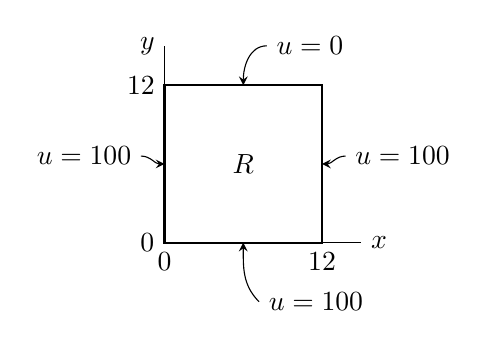
\begin{tikzpicture}
\draw(0,0)--(2.5,0)node[right]{$x$};
\draw(0,0)--(0,2.5)node[left]{$y$};
\draw[thick] (0,0)node[below]{$0$}node[left]{$0$} rectangle (2,2);
\draw(2,0)node[below]{$12$};
\draw(0,2)node[left]{$12$};
\draw(1,1)node{$R$};
\draw[stealth-] (0,1) to [out=180,in=0] ++(-0.3,0.1) node[left]{$u=100$};
\draw[stealth-] (1,0) to [out=-90,in=135]++(0.2,-0.75)node[right]{$u=100$};
\draw[stealth-] (2,1) to [out=0,in=180] ++(0.3,0.1) node[right]{$u=100$};
\draw[stealth-] (1,2) to [out=90,in=180] ++(0.3,0.5) node[right]{$u=0$};
\end{tikzpicture}
\caption*{(الف) دیا گیا مسئلہ}
\end{subfigure}%
\begin{subfigure}{0.45\textwidth}
\centering
\begin{tikzpicture}
\draw[thick] (0,0) rectangle (2,2);
\foreach \x in {1,2} {\draw(2/3*\x,0)--++(0,2);}
\foreach \y in {1,2} {\draw(0,2/3*\y)--++(2,0);}
\draw(2/3,0)node[ocirc]{}node[shift={(0.3cm,0.2cm)},font=\small]{$N_{10}$};
\draw(4/3,0)node[ocirc]{}node[shift={(0.3cm,0.2cm)},font=\small]{$N_{20}$};
\draw(0,2/3)node[ocirc]{}node[shift={(0.3cm,0.2cm)},font=\small]{$N_{01}$};
\draw(2/3,2/3)node[ocirc]{}node[shift={(0.3cm,0.2cm)},font=\small]{$N_{11}$};
\draw(4/3,2/3)node[ocirc]{}node[shift={(0.3cm,0.2cm)},font=\small]{$N_{21}$};
\draw(0,4/3)node[ocirc]{}node[shift={(0.3cm,0.2cm)},font=\small]{$N_{02}$};
\draw(2/3,4/3)node[ocirc]{}node[shift={(0.3cm,0.2cm)},font=\small]{$N_{12}$};
\draw(4/3,4/3)node[ocirc]{}node[shift={(0.3cm,0.2cm)},font=\small]{$N_{22}$};
\draw(2,2/3)node[ocirc]{};
\draw(2,4/3)node[ocirc]{};
\draw(1,0)node[below]{$u=100$};
\draw(1,2)node[above]{$u=0$};
\draw(0,1)node[above,rotate=90]{$u=100$};
\draw(2,1)node[below,rotate=90]{$u=100$};
\end{tikzpicture}
\caption*{(ب) جال اور جوڑ}
\end{subfigure}%
\caption{شکل برائے مثال \حوالہ{مثال_اعدادی_لیبمن_چادر_حراری}}
\label{شکل_مثال_اعدادی_لیبمن_چادر_حراری}
\end{figure}

حل:\quad
برقرار حال نتائج میں وقت بطور متغیر نہیں پایا جائے گا لہٰذا حراری مساوات
\begin{align*}
u_t=k^2(u_{xx}+u_{yy})
\end{align*}
سے مساوات لاپلاس حاصل ہو گی۔یوں ہمیں مسئلہ ڈرشلے حل کرنا ہو گا۔ہم شکل میں دکھائی گئی جال بچھاتے ہیں اور جوڑ \عددی{N_{11}}، \عددی{N_{21}}، \عددی{N_{12}}، \عددی{N_{22}} پر اسی ترتیب میں غور کرتے ہیں۔مساوات \حوالہ{مساوات_اعدادی_جزوی_عمومی_ڈ} سے درج ذیل لکھا جا سکتا ہے۔
\begin{gather}
\begin{aligned}\label{مساوات_اعدادی_نظام_لیبمن_الف}
-4u_{11}+u_{21}+u_{12}\phantom{+u_{13}}&=-200\\
u_{11}-4u_{21}\phantom{+u_{23}}+u_{22}&=-200\\
u_{11}\phantom{u_{22}}-4u_{12}+u_{22}&=-100\\
u_{21}+u_{12}-4u_{22}&=-100
\end{aligned}
\end{gather}
عملاً اتنے کم مساوات کو آپ گاوسی اسقاط سے حل کرے ہوئے درج ذیل حاصل کریں گے۔
\begin{align*}
u_{11}=u_{21}=87.5,\quad u_{12}=u_{22}=62.5
\end{align*}
ایک اعشاریہ  تک (زیادہ درست) جوابات \عددی{88.1} اور \عددی{61.9} ہیں (جنہیں فوریئر تسلسل سے حاصل کیا گیا)۔یوں خلل \عددی{\SI{1}{\percent}} کے لگ بھگ ہے جو اتنے چوڑے جال کے لئے حیرت کن بات ہے۔ زیادہ مساواتوں کی صورت میں نظام کو ترکیب لیبمن سے حل کیا جائے گا۔ایسا کرتے ہوئے مساوات \حوالہ{مساوات_اعدادی_نظام_لیبمن_الف} کو پہلے درج ذیل صورت میں لکھتے ہیں۔
\begin{gather}
\begin{aligned}\label{مساوات_اعدادی_نظام_لیبمن_ب}
u_{11}&=\phantom{u_{23}}0.25u_{21}+0.25u_{12}\phantom{u_{32}}+50\\
u_{21}&=0.25u_{11}\phantom{u_{23}+u_{32}}+0.25u_{22}+50\\
u_{12}&=0.25u_{11}\phantom{u_{23}+u_{21}}+0.25u_{22}+25\\
u_{22}&=\phantom{u_{12}+u_{23}}0.25u_{21}+0.25u_{12}\phantom{u_{21}}+25
\end{aligned}
\end{gather} 
انہیں اب ترکیب گاوس زائڈل میں استعمال کیا جاتا ہے۔\عددی{u_{11}=w}، \عددی{u_{21}=x}، \عددی{u_{12}=y}، \عددی{u_{22}=z} لیتے ہوئے یہ  حصہ  \حوالہ{حصہ_خطی_اعدادی_حل_بذریعہ_اعادہ} میں مساوات دیتی ہیں جہاں ابتدائی قیمتیں \عددی{100}، \عددی{100}، \عددی{100} لیتے ہوئے اس کو  حل کیا گیا ہے۔جوڑ پر قیمتوں کا بہتر اندازہ لگانے سے نتائج زیادہ آسانی سے حاصل کیے جا سکتے ہیں۔آپ تسلی کر سکتے ہیں کہ اس نظام کا حل \عددی{u_{11}=u_{21}=87.5} اور \عددی{u_{12}=u_{22}=62.5} ہے۔

آسانی پیدا کرنے کی تراکیب جاننے کے لئے سوال \حوالہ{سوال_اعدادی_تشاکل_آسانی} دیکھیں۔

\موٹا{رائے:} اگر \عددی{h=\tfrac{l}{n}} منتخب کیا جائے جہاں \عددی{R} کی ایک طرف کی لمبائی \عددی{l} ہو اور \عددی{(n-1)^2} جوڑ کو صف در صف لیا جائے  یعنی پہلے صف \عددی{N_{11},N_{21},\cdots,N_{n1}} کے بعد دوسرا صف \عددی{N_{12},N_{22},\cdots,N_{n2}} اور اس کے بعد تیسرا صف، \نقطے  لیا جائے تب نظام کا \عددی{(n-1)^2\times(n-1)^2} عددی سر قالب \عددی{\bM{A}}  درج ذیل ہو گا
\begin{align}\label{مساوات_اعدادی_نظام_لیبمن_پ}
\text{(الف)}\quad
\bM{A}=
\begin{bmatrix} 
\bM{B}&\bM{I}&&&&&\\  
\bM{I}&\bM{B}&\bM{I}&&&&\\  
\vdots\\
&&&&\bM{I}&\bM{B}&\bM{I}\\  
&&&&&\bM{I}&\bM{B}
\end{bmatrix}
\end{align} 
جہاں
\begin{align*}\tag{\ref{مساوات_اعدادی_نظام_لیبمن_پ}}
\text{(ب)}\quad 
\bM{B}=
\begin{bmatrix} 
-4&1&&&&&\\  
1&-4&1&&&&\\  
\vdots\\
&&&&1&-4&1\\  
&&&&&1&-4
\end{bmatrix}
\end{align*} 
ہے جو \عددی{(n-1)\times (n-1)} قالب  ہے۔یہ ثابت کیا جا سکتا ہے کہ \عددی{\bM{A}} غیر نادر ہو گا۔
\انتہا{مثال}
%===============================

ایسا قالب جس کے تمام غیر صفر اجزاء مرکزی وتر اور مرکزی وتر کے متوازی ترچھی لکیروں پر واقع ہوں (ان لکیروں اور مرکزی وتر کے بیچ ایسی ترچھی لکیریں ہو سکتی ہیں جن کے اجزاء صفر ہوں) کو \اصطلاح{پٹی قالب}\فرہنگ{قالب!پٹی}\حاشیہب{band matrix}\فرہنگ{matrix!band} کہتے ہیں۔مثال کے طور پر   مساوات \حوالہ{مساوات_اعدادی_نظام_لیبمن_پ} میں \عددی{\bM{A}} پٹی قالب ہے۔اگرچہ گاوسی اسقاط پٹی میں صفروں  کو برقرار نہیں رکھتا ہے البتہ یہ پٹی کے باہر غیر صفر اجزاء بھی پیدا نہیں کرتا ہے۔یوں عددی سر قالب کی پٹی صورت سود مند ثابت ہوتی ہے۔مساوات \حوالہ{مساوات_اعدادی_نظام_لیبمن_پ} میں جوڑ کی ترتیب یوں منتخب کی گئی کہ پٹی قالب حاصل ہو۔


\جزوحصہ{بدلتی رخ خفی ترکیب}
ایسا قالب جس میں تمام غیر صفر اجزاء مرکزی وتر یا مرکزی وتر کے ساتھ ملے ہوئے خانوں میں پائے جاتے ہوں کو \اصطلاح{سہ وتری قالب}\فرہنگ{وتر!سہ وتری قالب}\حاشیہب{tridiagonal matrix}\فرہنگ{matrix!tridiagonal} کہتے ہیں۔ایسی صورت میں گاوسی اسقاط کا استعمال خصوصی طور پر سادہ ثابت ہوتا ہے۔

اس سے سوال پیدا ہوتا ہے کہ آیا مساوات لاپلاس یا مساوات پوئسن کے مسئلہ ڈرشلے کا اعدادی حل تلاش کرنے کی خاطر ہم مساوات کا ایسا نظام حاصل کر سکتے ہیں جس کا عددی سر  قالب سہ وتری ہو۔جی ہاں ایسا ممکن ہے اور سہ وتری قالب حاصل کرنے کی ایک مقبول ترکیب \اصطلاح{بدلتی رخ خفی ترکیب}\فرہنگ{ترکیب!بدلتی رخ خفی }\حاشیہب{alternating direction implicit method, ADI}\فرہنگ{ADI!alternating direction implicit method} کہلاتی ہے۔مساوات \حوالہ{مساوات_اعدادی_جزوی_عمومی_ح} کی نقش کو دیکھ کر معلوم ہوتا ہے کہ اگر صف میں صرف یہی تین نقطے ہوں (یا قطار میں یہی تین نقطے ہوں) تب سہ وتری قالب حاصل ہو گی۔ یوں ہم مساوات \حوالہ{مساوات_اعدادی_جزوی_عمومی_ڈ}  کو درج ذیل صورت میں لکھتے ہیں
\begin{align}\label{مساوات_اعدادی_بدلتی_رخ_خفی_الف}
\text{(الف)}\quad u_{i-1,j}-4u_{ij}+u_{i+1,j}=-u_{i,j-1}-u_{i,j+1}
\end{align}
تا کہ بایاں ہاتھ صف \عددی{j} کا حصہ ہو اور دایاں ہاتھ قطار  \عددی{i} کا حصہ ہو۔ظاہر ہے کہ ہم مساوات \حوالہ{مساوات_اعدادی_جزوی_عمومی_ڈ}  کو
\begin{align*}
\text{(ب)}\quad u_{i,j-1}-4u_{ij}+u_{i,j+1}=-u_{i-1,j}-u_{i+1,j}\tag{\ref{مساوات_اعدادی_بدلتی_رخ_خفی_الف}}
\end{align*}
بھی لکھ سکتے ہیں جہاں بایاں ہاتھ قطار \عددی{i} کا حصہ ہو گا اور دایاں ہاتھ صف \عددی{j} کا حصہ ہو گا۔ہم بدلتی رخ خفی ترکیب کو بار بار دہرا کر آگے  بڑھتے ہیں۔ہم ہر جوڑ پر ابتدائی قیمت \عددی{u^{(0)}_{ij}} سے شروع کرتے ہیں۔ہر قدم پر ہم تمام جوڑوں پر نئی قیمتیں حاصل کرتے ہیں۔ایک قدم میں ہم مساوات \حوالہ{مساوات_اعدادی_بدلتی_رخ_خفی_الف}-الف سے اخذ کلیہ توالی استعمال کرتے ہیں جبکہ اگلی قدم میں ہم مساوات \حوالہ{مساوات_اعدادی_بدلتی_رخ_خفی_الف}-ب سے اخذ کلیہ توالی استعمال کرتے ہیں اور اسی طرح متواتر یہی کلیات استعمال کرتے ہوئے بڑھتے ہیں۔ یوں اگر  ہم \عددی{u^{(m)}_{ij}}  حاصل کر چکے ہوں، تب مساوات \حوالہ{مساوات_اعدادی_بدلتی_رخ_خفی_الف}-الف کے دائیں ہاتھ میں  \عددی{u^{(m)}_{ij}} پر کر کے  ہم بائیں ہاتھ کو \عددی{u^{(m+1)}_{ij}} کے لئے حل کریں گے یعنی:
\begin{align}\label{مساوات_اعدادی_بدلتی_رخ_خفی_ب}
\text{(الف)}\quad u^{(m+1)}_{i-1,j}-4u^{(m+1)}_{ij}+u^{(m+1)}_{i+1,j}=-u^{(m)}_{i,j-1}-u^{(m)}_{i,j+1}
\end{align}
ہم مقررہ \عددی{j} یعنی مقررہ صف \عددی{j} کے  تمام جوڑوں کے لئے یہ کلیہ استعمال کرتے ہیں جس سے  \عددی{N}  عدد خطی مساوات کا نظام حاصل ہو گا جس میں \عددی{N} نا معلوم متغیرات (یعنی جوڑوں پر \عددی{u} کی نئی تخمینی قیمتیں) ہوں گی، اور جہاں مقررہ صف میں  اندرونی نقطوں کی تعداد \عددی{N} ہے۔مساوات \حوالہ{مساوات_اعدادی_بدلتی_رخ_خفی_ب}-الف میں نا صرف گزشتہ قدم کی تخمینی قیمتیں بلکہ سرحدی قیمتیں بھی شامل ہیں۔ ہم (مقررہ \عددی{j} کے لئے) گاوسی اسقاط سے مساوات \حوالہ{مساوات_اعدادی_بدلتی_رخ_خفی_ب}-الف حل کرتے ہیں۔اس کے بعد ہم اگلی صف کے لئے \عددی{N} عدد مساوات کا نظام حاصل کر کے اس کو  گاوسی اسقاط سے حل کرتے ہیں۔اسی طرح چلتے ہوئے ہم آخری صف کے لئے بھی نتائج حاصل کرتے ہیں۔اگلے قدم میں ہم رخ تبدیل کرتے ہیں اور \عددی{u^{(m+1)}_{ij}} کو مساوات \حوالہ{مساوات_اعدادی_بدلتی_رخ_خفی_الف}-ب کے دائیں ہاتھ میں پر کرتے ہوئے درج ذیل  کلیہ اخذ کرتے ہوئے
\begin{align*}
\text{ب}\quad u^{(m+2)}_{i,j-1}-4^{(m+2)}_{ij}+u^{(m+2)}_{i,j+1}=-u^{(m+1)}_{i-1,j}-u^{(m+1)}_{i+1,j}\tag{\ref{مساوات_اعدادی_بدلتی_رخ_خفی_ب}}
\end{align*}
 اس سے  قطار در قطار نئی تخمینی قیمتیں \عددی{u^{(m+2)}_{ij}} حاصل کرتے ہیں۔ایسا کرتے ہوئے گزشتہ تخمینی قیمتیں \عددی{u^{(m+1)}_{ij}} اور سرحدی قیمتیں استعمال کی جاتی ہیں۔ہر مقررہ \عددی{j}، یعنی ہر قطار کے لئے \عددی{M} خطی مساوات کا نظام حاصل ہو گا (جہاں قطار میں اندرونی نقطوں کی تعداد \عددی{M} ہے) جس کو گاوسی اسقاط سے حل کرتے ہوئے  \عددی{M} نا معلوم متغیرات کی تخمینی قیمتیں حاصل کی جاتی ہیں۔اس کے بعد اگلی قطار کے لئے نظام حاصل کر کے حل کیا جاتا ہے۔اسی طرح آخری قطار تک کی تمام اندرونی جوڑوں پر تخمینی قیمتیں حاصل کی جاتی ہیں۔ 

بدلتی رخ خفی ترکیب کو سمجھنے کی خاطر ایک مثال پیش کرتے ہیں۔(حقیقت میں ایسی مثال کو گاوسی اسقاط سے حل کیا جائے گا۔) اس کے بعد ہم بدلتی رخ خفی ترکیب میں ارتکاز کی بہتری پر غور کریں گے۔

%=======================
\ابتدا{مثال}\شناخت{مثال_اعدادی_ڈرشلے_بدلتی_رخ_مخفی}\quad \موٹا{مسئلہ ڈرشلے۔ بدلتی رخ خفی ترکیب}\\
بدلتی رخ خفی ترکیب میں ابتدائی قیمتیں \عددی{100}، \عددی{100}، \عددی{100}، \عددی{100} لیتے ہوئے مثال \حوالہ{مثال_اعدادی_لیبمن_چادر_حراری} کو دوبارہ حل کریں۔جسامت جال وہی رکھیں۔\\
حل:\quad
شکل \حوالہ{شکل_مثال_اعدادی_لیبمن_چادر_حراری}-ب  جو سرحدی قیمتیں دیتی ہے پر نظر رکھیں۔مساوات \حوالہ{مساوات_اعدادی_بدلتی_رخ_خفی_ب}-الف میں \عددی{m=0} لیتے ہوئے ہم  پہلی تخمینی قیمتیں \عددی{u^{(1)}_{11}}، \عددی{u^{(1)}_{21}}، \عددی{u^{(1)}_{12}}، \عددی{u^{(1)}_{22}}  حاصل کرتے ہیں۔ہم سرحدی قیمتوں کو مساوات \حوالہ{مساوات_اعدادی_بدلتی_رخ_خفی_ب}-الف میں بغیر بالائی اشاریہ لکھتے ہیں تا کہ ان پر نظر رکھنا آسان ہو اور یہ واضح کرنے کی خاطر کہ دہرانے کے دوران یہ قیمتیں تبدیل نہیں ہوتی ہیں۔۔مساوات \حوالہ{مساوات_اعدادی_بدلتی_رخ_خفی_ب}-الف میں \عددی{m=0} لیتے ہوئے  \عددی{j=1} (پہلی صف) کے لئے درج ذیل نظام حاصل ہو گا
\begin{align*}
(i=1)\quad u_{01}-4u^{(1)}_{11}+u^{(1)}_{21}\phantom{+u^{(1)}_{32}}&=-u_{10}-u^{(0)}_{12}\\
(i=2)\quad\quad  \quad u^{(1)}_{11}-4u^{(1)}_{21}+u_{31}&=-u_{20}-u^{(0)}_{22}
\end{align*}
جس کا حل \عددی{u^{(1)}_{11}=u^{(1)}_{21}=100} ہے۔ دوسری صف یعنی \عددی{j=2} کے لئے  مساوات \حوالہ{مساوات_اعدادی_بدلتی_رخ_خفی_ب}-الف سے
\begin{align*}
(i=1)\quad u_{02}-4u^{(1)}_{12}+u^{(1)}_{22}\phantom{+u^{(1)}_{23}}&=-u^{(0)}_{11}-u_{13}\\
(i=2)\quad\quad\quad u^{(1)}_{12}-4u^{(1)}_{22}+u_{32}&=-u^{(0)}_{21}-u_{23}
\end{align*}
حاصل ہو گا جس کا حل \عددی{u^{(1)}_{12}=u^{(1)}_{22}=66.667} ہے۔

اب \عددی{m=1} لیتے ہوئے درج بالا حاصل کردہ تخمینی قیمتیں اور سرحدی قیمتیں استعمال کرتے ہوئے  دوسری تخمینی قیمتیں \عددی{u^{(2)}_{11}}، \عددی{u^{(2)}_{21}}، \عددی{u^{(2)}_{12}}، \عددی{u^{(2)}_{22}} مساوات \حوالہ{مساوات_اعدادی_بدلتی_رخ_خفی_ب}-ب  سے حاصل کی جاتی ہیں۔یوں \عددی{i=1} (پہلی قطار) کے لئے  مساوات \حوالہ{مساوات_اعدادی_بدلتی_رخ_خفی_ب}-ب سے  نظام
\begin{align*}
(j=1)\quad u_{10}-4u^{(2)}_{11}+u^{(2)}_{12}\phantom{+u^{(2)}_{23}}&=-u_{01}-u^{(1)}_{21}\\
(j=2)\quad \quad \quad u^{(2)}_{11}-4u^{(2)}_{12}+u_{13}&=-u_{02}-u^{(1)}_{22}
\end{align*}
حاصل ہو گا جس کا حل \عددی{u^{(2)}_{11}=91.11}، \عددی{u^{(2)}_{12}=64.44} ہے۔ دوسری قطار یعنی \عددی{i=2} کے لئے  مساوات \حوالہ{مساوات_اعدادی_بدلتی_رخ_خفی_ب}-ب سے  نظام
\begin{align*}
(j=1)\quad u_{20}-4u^{(2)}_{21}+u^{(2)}_{22}\phantom{+u^{(2)}_{23}}&=-u^{(1)}_{11}-u_{31}\\
(j=2)\quad \quad \quad u^{(2)}_{21}-4u^{(2)}_{22}+u_{23}&=-u^{(1)}_{12}-u_{32}
\end{align*}
حاصل ہو گا جس کا حل \عددی{u^{(2)}_{21}=91.11}، \عددی{u^{(2)}_{22}=64.44} ہے۔

اس مثال میں جو محض  بدلتی رخ خفی ترکیب سمجھنے کی خاطر استعمال کی گئی، دوسری تخمینی قیمتوں کی درستگی  تقریباً حصہ \حوالہ{حصہ_خطی_اعدادی_حل_بذریعہ_اعادہ} کے دو قدم گاوس زائڈل کے برابر ہے 
(جہاں \عددی{u_{11}=w}، \عددی{u_{21}=x}، \عددی{u_{12}=y}، \عددی{u_{22}=z} ہیں)۔  
\begin{align*}
\centering
\begin{array}{r c c c c}
\hline
&u_{11}&u_{21}&u_{12}&u_{22}\\
\hline\Tstrut
\text{\RL{بدلتی رخ خفی ترکیب، دوسری تخمین}}&91.11&91.11&64.44&64.44\\
\text{\RL{گاوس زائڈل، دوسری تخمین}}&93.75&90.62&65.62&64.06\\
\text{\RL{مساوات \حوالہ{مساوات_اعدادی_نظام_لیبمن_الف} کا اصل حل}}&87.50&87.50&62.50&62.50\\
\hline
\end{array}
\end{align*}
\انتہا{مثال}
%=============================

مقدار معلوم \عددی{p} متعارف کرتے ہوئے مساوات \حوالہ{مساوات_اعدادی_جزوی_عمومی_ڈ} کو
\begin{align}\label{مساوات_اعدادی_نیا_روپ_الف}
\text{(الف)}\quad u_{i-1,j}-(2+p)u_{ij}+u_{i+1,j}=-u_{i,j-1}+(2-p)u_{ij}-u_{i,j+1}
\end{align}
اور
\begin{align*}
\text{(ب)}\quad u_{i,j-1}-(2+p)u_{ij}+u_{i,j+1}=-u_{i-1,j}+(2-p)u_{ij}-u_{i+1,j}\tag{\ref{مساوات_اعدادی_نیا_روپ_الف}}
\end{align*}
روپ میں لکھ جا سکتا ہے جس سے  بدلتی رخ خفی ترکیب کے زیادہ عمومی کلیات
\begin{align}\label{مساوات_اعدادی_نیا_روپ_ب}
\text{(الف)}\quad u^{(m+1)}_{i-1,j}-(2+p)u^{(m+1)}_{ij}+u^{(m+1)}_{i+1,j}=-u^{(m)}_{i,j-1}+(2-p)u^{(m)}_{ij}-u^{(m)}_{i,j+1} 
\end{align}
اور
\begin{align*}
\text{(ب)}\quad u^{(m+2)}_{i,j-1}-(2+p)u^{(m+2)}_{ij}+u^{(m+2)}_{i,j+1}=-u^{(m+1)}_{i-1,j}+(2-p)u^{(m+1)}_{ij}-u^{(m+1)}_{i+1,j}\tag{\ref{مساوات_اعدادی_نیا_روپ_ب}}
\end{align*}
اخذ ہوتے ہیں۔  ان میں \عددی{p=2} پر کرنے سے  مساوات \حوالہ{مساوات_اعدادی_بدلتی_رخ_خفی_ب} حاصل ہوتے ہیں۔مقدار معلوم \عددی{p} سے  ارتکاز میں بہتری پیدا کی جا سکتی ہے۔یہ ثابت کیا جا سکتا ہے کہ بدلتی رخ خفی ترکیب مثبت \عددی{p} کے لئے مرتکز ہو گی اور ارتکاز کی شرح زیادہ سے زیادہ حاصل کرنے کے لئے \عددی{p} کی بہترین قیمت 
\begin{align}\label{مساوات_اعدادی_موزوں_مقدار_معلوم}
p_o=2\sin \frac{\pi}{C}
\end{align}
ہے جہاں \عددی{C} کی قیمت \عددی{M+1} اور \عددی{N+1} میں زیادہ بڑی قیمت کے برابر  ہے۔ مزید بہتر نتائج حاصل کرنے  کی خاطر \عددی{p} کی قیمت کو ہر ایک قدم کے دوران  مختلف رکھا جا سکتا ہے۔

%==================
\حصہء{سوالات}

%=========================
\ابتدا{سوال}\quad
مساوات \حوالہ{مساوات_اعدادی_جزوی_عمومی_ٹ}-ب اخذ کریں۔
\انتہا{سوال}
%=========================
\ابتدا{سوال}\quad
مساوات \حوالہ{مساوات_اعدادی_جزوی_عمومی_ث}-ب اخذ کریں۔
\انتہا{سوال}
%=========================
\ابتدا{سوال}\شناخت{سوال_اعدادی_ثبوت_درکار}\quad
مساوات \حوالہ{مساوات_اعدادی_جزوی_عمومی_ث}-پ اخذ کریں۔\\
جواب:\quad
$u_{xy}(x,y)\approx \tfrac{1}{2k}[u_x(x,y+k)-u_x(x,y-k)]$
میں درج ذیل پر کریں۔\\
$u_x(x,y\mp k)\approx \tfrac{1}{2h}[u(x+h,y\mp k)-u(x-h,y\mp k)]$
\انتہا{سوال}
%=========================
\ابتدا{سوال}\شناخت{سوال_اعدادی_تشاکل_آسانی}\quad \موٹا{تشاکل کا استعمال}\\
مثال \حوالہ{مثال_اعدادی_لیبمن_چادر_حراری} کی سرحدی قیمتوں کو دیکھ کر فیصلہ کریں کہ \عددی{u_{21}=u_{11}} اور \عددی{u_{22}=u_{12}} ہو گا۔دکھائیں کہ اس سے دو مساوات کا نظام حاصل ہو گا۔اس نظام کو حل کریں۔
\انتہا{سوال}
%========================
\ابتدا{سوال}\quad
\عددی{h=6} لیتے ہوئے مثال \حوالہ{مثال_اعدادی_لیبمن_چادر_حراری} میں \عددی{u_{11}} حاصل کریں۔اس کا بالکل درست قیمت \عددی{75} کے ساتھ موازنہ کریں۔\\
جواب:\quad
$75$
\انتہا{سوال}
%====================
\ابتدا{سوال}\quad
\عددی{h=3} لیتے ہوئے مثال \حوالہ{مثال_اعدادی_لیبمن_چادر_حراری} حل کریں۔
\انتہا{سوال}
%====================
\ابتدا{سوال}\شناخت{سوال_اعدادی_برقی_سکون_الف}\quad
شکل \حوالہ{شکل_سوال_اعدادی_برقی_سکون_الف} میں \عددی{N_{11}}، \عددی{N_{12}}، \عددی{N_{13}} پر ساکن برقی مخفی قوہ کی تخمینی قیمت تلاش کریں۔یہ نقطے موصل چادروں کے درمیان پائے جاتے ہیں (جو شکل میں بطور مستطیل نظر آتے ہیں) اور جن پر برقی مخفی قوہ \عددی{\SI{0}{\volt}} اور \عددی{\SI{100}{\volt}} ہے۔دکھایا گیا جال اور گاوسی اسقاط استعمال کریں۔
\begin{figure}
\centering
\begin{minipage}{0.45\textwidth}
\centering
\begin{tikzpicture}
\draw[thick] (0,3.9)--(0,0)node[below]{$0$}node[left]{$0$}--(2,0)node[below]{$2$}--(2,3.9);
\draw[thick] (0,4)node[left]{$4$}--++(2,0);
\foreach \y in {1,2,3}{\draw(0,\y)--++(2,0);}
\draw(1,0)--(1,4);
\draw(1,0)node[below]{$1$};
\draw(2.2,0)--++(0.5,0)node[below]{$x$};
\draw(0,4.3)--++(0,0.5)node[left]{$y$};
\draw(1,1)node[ocirc]{}node[shift={(0.3,0.2)},font=\small]{$N_{11}$};
\draw(1,2)node[ocirc]{}node[shift={(0.3,0.2)},font=\small]{$N_{12}$};
\draw(1,3)node[ocirc]{}node[shift={(0.3,0.2)},font=\small]{$N_{13}$};
\draw[stealth-] (0,1.75) to [out=-160, in =45]++(-0.3,-0.3) node[left]{$u=0$};
\draw[stealth-] (2,1.75) to [out=-20, in =135]++(0.3,-0.3) node[right]{$u=0$};
\draw[stealth-] (0.75,0) to [out=-120, in =45]++(-0.3,-0.75) node[left]{$u=0$};
\draw[stealth-] (0.75,4) to [out=60, in =-160]++(0.3,0.3) node[right]{$u=100$};
\end{tikzpicture}
\caption{شکل برائے سوال \حوالہ{سوال_اعدادی_برقی_سکون_الف}}
\label{شکل_سوال_اعدادی_برقی_سکون_الف}
\end{minipage}\hfill
\begin{minipage}{0.45\textwidth}
\centering
\begin{tikzpicture}
\draw(3.2,0)--++(0.5,0)node[below]{$x$};
\draw(0,3.2)--++(0,0.5)node[left]{$y$};
\foreach \x in {1,2}{\draw(\x,0)node[below]{$\x$}--++(0,3);}
\foreach \y in {1,2}{\draw(0,\y)node[left]{$\y$}--++(3,0);}
\draw[thick](0,0)node[below]{$0$}node[left]{$0$} rectangle (3,3);
\draw(1,1)node[ocirc]{}node[shift={(0.3,0.2)},font=\small]{$N_{11}$};
\draw(2,1)node[ocirc]{}node[shift={(0.3,0.2)},font=\small]{$N_{21}$};
\draw(1,2)node[ocirc]{}node[shift={(0.3,0.2)},font=\small]{$N_{12}$};
\draw(2,2)node[ocirc]{}node[shift={(0.3,0.2)},font=\small]{$N_{22}$};
\draw(3,0)node[below]{$3$};
\draw(0,3)node[left]{$3$};
\end{tikzpicture}
\caption{شکل برائے سوال \حوالہ{سوال_اعدادی_برقی_سکون_ب}، سوال \حوالہ{سوال_اعدادی_برقی_سکون_پ} اور سوال \حوالہ{سوال_اعدادی_برقی_سکون_ث}}
\label{شکل_سوال_اعدادی_برقی_سکون_ب}
\end{minipage}
\end{figure}

جواب:\quad
$1.96,\,7.86,\,29.46$
\انتہا{سوال}
%==========================
\ابتدا{سوال}\شناخت{سوال_اعدادی_برقی_سکون_ب}\quad
شکل \حوالہ{شکل_سوال_اعدادی_برقی_سکون_ب} میں نچلی چادر پر \عددی{u=x^3}، دائیں چادر پر \عددی{u=27-9y^2}، بالائی چادر پر \عددی{u=x^3-27x} اور بائیں چادر پر \عددی{u=0} تصور کرتے ہوئے مخفی قوہ \عددی{u(x,y)} کو گاوسی اسقاط سے  تلاش کریں۔
\انتہا{سوال}
%==========================
\ابتدا{سوال}\شناخت{سوال_اعدادی_برقی_سکون_پ}\quad
شکل \حوالہ{شکل_سوال_اعدادی_برقی_سکون_ب} میں نچلی چادر پر \عددی{u=x^4}، دائیں چادر پر \عددی{u=81-54y^2+y^4}، بالائی چادر پر \عددی{u=x^4-54x^2+81} اور بائیں چادر پر \عددی{u=y^4} تصور کرتے ہوئے مخفی قوہ \عددی{u(x,y)} کو گاوسی اسقاط سے  تلاش کریں۔تصدیق کریں کہ اس مسئلے کا حل \عددی{u(x,y)=x^4-6x^2y^2+y^4} ہے اور خلل تلاش کریں۔\\
جواب:\quad
$-2,\,-5,\,-5,\,-62$
\انتہا{سوال}
%==========================
\ابتدا{سوال}\شناخت{سوال_اعدادی_برقی_سکون_ت}\quad
شکل \حوالہ{شکل_سوال_اعدادی_برقی_سکون_ت} میں مخفی قوہ کو (الف) چوڑی جال پر، (ب) باریک جال پر،  گاوسی اسقاط کی مدد سے تلاش کریں۔ اشارہ۔ باریک جال میں تشاکل استعمال کریں اور  ان دو نقطوں پر جہاں  سرحدی مخفی قوہ میں چھلانگ پائی جاتی ہے وہاں مخفی قوہ کو \عددی{\SI{0}{\volt}}  (یعنی \عددی{\SI{-110}{\volt}} اور \عددی{\SI{110}{\volt}} کی اوسط)  فرض کریں۔ 
\begin{figure}
\centering
\begin{subfigure}{0.5\textwidth}
\centering
\begin{tikzpicture}
\draw[thick] (0,1.55)--(0,3)--(2,3)--(2,1.55)++(0,-0.1)--(2,0)--(0,0)--(0,1.45);
\draw(1,0)node[below,font=\small]{$u=\SI{-110}{\volt}$};
\draw(1,3)node[above,font=\small]{$u=\SI{110}{\volt}$};
\draw(0,0.75)node[left,font=\small]{$u=\SI{-110}{\volt}$};
\draw(0,2.25)node[left,font=\small]{$u=\SI{110}{\volt}$};
\draw(2,0.75)node[right,font=\small]{$u=\SI{-110}{\volt}$};
\draw(2,2.25)node[right,font=\small]{$u=\SI{110}{\volt}$};
\foreach \x in {1}{\draw(\x,0)--++(0,3);}
\foreach \y in {1,2}{\draw(0,\y)--++(2,0) (1,\y)node[ocirc]{}node[shift={(0.3,0.2)},font=\small]{$N_{1\y}$};}
\end{tikzpicture}
\end{subfigure}%
\begin{subfigure}{0.5\textwidth}
\centering
\begin{tikzpicture}
\draw[thick] (0,1.55)--(0,3)--(2,3)--(2,1.55)++(0,-0.1)--(2,0)--(0,0)--(0,1.45);
\draw(1,0)node[below,font=\small]{$u=\SI{-110}{\volt}$};
\draw(1,3)node[above,font=\small]{$u=\SI{110}{\volt}$};
\draw(0,0.75)node[left,font=\small]{$u=\SI{-110}{\volt}$};
\draw(0,2.25)node[left,font=\small]{$u=\SI{110}{\volt}$};
\draw(2,0.75)node[right,font=\small]{$u=\SI{-110}{\volt}$};
\draw(2,2.25)node[right,font=\small]{$u=\SI{110}{\volt}$};
\foreach \x in {0.5,1,1.5}{\draw(\x,0)--++(0,3);}
\foreach \y in {1,2,3,4,5}{\draw(0,\y/2)--++(2,0) (0.5,\y/2)node[ocirc]{}node[shift={(0.2,0.2)},font=\small]{${1\y}$}   (1,\y/2)node[ocirc]{}node[shift={(0.2,0.2)},font=\small]{${2\y}$}  (1.5,\y/2)node[ocirc]{}node[shift={(0.2,0.2)},font=\small]{${3\y}$};}
\end{tikzpicture}
\end{subfigure}%
\caption{شکل برائے سوال \حوالہ{سوال_اعدادی_برقی_سکون_ت}}
\label{شکل_سوال_اعدادی_برقی_سکون_ت}
\end{figure}
\انتہا{سوال}
%============================
\ابتدا{سوال}\quad
ترکیب گاوس زائڈل میں \عددی{0,0} سے ابتدا کرتے ہوئے کتنے قدم بعد سوال \حوالہ{سوال_اعدادی_برقی_سکون_ت} میں چوڑی جال کے نتائج پانچ ملحوظ ہندسوں تک درست ہوں گے؟ باریک جال کی صورت میں ارتکاز کی شرح بہت کم ہو گی۔کیا مساوات کی نظام کو دیکھ کر آپ اس کی وجہ بتا سکتے ہیں۔\\
جواب:\quad
پانچ قدم
\انتہا{سوال}
%===========================
\ابتدا{سوال}\شناخت{سوال_اعدادی_برقی_سکون_ث}
شکل \حوالہ{شکل_سوال_اعدادی_برقی_سکون_ب} میں بالائی چادر پر \عددی{u=\sin \tfrac{1}{3}\pi x} جبکہ باقی چادروں پر \عددی{u=0} ہے۔تصدیق کریں کہ اس کا بالکل درست حل \عددی{u(x,y)=\tfrac{\sin\tfrac{1}{3}\pi x\sinh\tfrac{1}{3}\pi y}{\sinh \pi}} ہے۔اعدادی حل حاصل کرتے ہوئے خلل کا تخمینہ لگائیں۔
\انتہا{سوال}
%=========================
\ابتدا{سوال}\شناخت{سوال_اعدادی_برقی_سکون_ج}\quad 
مساوات \حوالہ{مساوات_اعدادی_نظام_لیبمن_ب} میں دیے گئے نظام کے لئے مساوات \حوالہ{مساوات_اعدادی_نظام_لیبمن_پ} کی تصدیق کریں۔دکھائیں کہ مساوات \حوالہ{مساوات_اعدادی_نظام_لیبمن_ب} میں \عددی{\bM{A}} غیر نادر ہے۔ 
\انتہا{سوال}
%========================
\ابتدا{سوال}\شناخت{سوال_اعدادی_برقی_سکون_چ}\quad
شکل \حوالہ{شکل_سوال_اعدادی_برقی_سکون_ب} کی جال استعمال کرتے ہوئے سوال \حوالہ{سوال_اعدادی_برقی_سکون_ث} کے مسئلہ ڈرشلے  کو بدلتی رخ مخفی ترکیب سے دو قدم تک حل کریں۔  ابتدائی قیمتیں صفر لیں۔
\انتہا{سوال}
%===================
\ابتدا{سوال}\شناخت{سوال_اعدادی_برقی_سکون_ح}\quad
مقدار معلوم \عددی{p} (مساوات \حوالہ{مساوات_اعدادی_موزوں_مقدار_معلوم}) کی موزوں قیمت  سوال \حوالہ{سوال_اعدادی_برقی_سکون_چ} کے لئے تلاش کریں۔\عددی{p_0=1.7} لیتے ہوئے مساوات \حوالہ{مساوات_اعدادی_نیا_روپ_ب} میں دیے گئے بدلتی رخ مخفی کلیات سے سوال  \حوالہ{سوال_اعدادی_برقی_سکون_چ} کو ایک قدم تک حل کریں۔ایک قدم کے بعد سوال \حوالہ{سوال_اعدادی_برقی_سکون_چ} کی پہلی قدم کی قیمتوں \عددی{0.077} اور \عددی{0.308} کے ساتھ موازنہ کرتے ہوئے ارتکاز میں بہتری کی تصدیق کریں۔ابتدائی قیمتیں صفر لیں۔\\
جواب:\quad
$\sqrt{3}u_{11}=u_{21}=0.0859,\, u_{12}=u_{22}=0.3180$
(چار اعشاریہ درست نتائج 
$0.1083,\,0.3248$
ہیں۔) 
\انتہا{سوال}
%========================
\ابتدا{سوال}\quad
\عددی{p=0} لینے سے مساوات \حوالہ{مساوات_اعدادی_نیا_روپ_ب} کے کلیات کارآمد نہیں رہتے ہیں۔یہ دیکھنے کی خاطر انہیں استعمال کرتے ہوئے مثال \حوالہ{مثال_اعدادی_ڈرشلے_بدلتی_رخ_مخفی} کو دو قدم تک حل کریں۔مثال میں دیا گیا جال اور ابتدائی قیمتیں استعمال کریں۔نتیجہ کیا حاصل ہوتا ہے؟
\انتہا{سوال}
%====================

\حصہ{مسئلہ نیومن اور مخلوط سرحدی قیمت مسئلہ۔ غیر منظم سرحد}
ہم \عددی{xy} مستوی کے خطہ \عددی{R} میں بیضوی مساوات کی سرحدی قیمت مسئلہ کے اعدادی حل پر بحث جاری رکھتے ہیں۔مسئلہ ڈرشلے پر گزشتہ حصے میں غور کیا گیا ہے۔نیومن اور مخلوط مسئلوں میں ہمیں نئی صورت حال کا سامنا ہوتا ہے چونکہ سرحد کے کچھ مقامات پر ہمیں \عددی{u} کی بجائے  \عددی{u_n=\tfrac{\partial u}{\partial n}} دیا گیا ہو گا لہٰذا سرحد کی ان مقامات پر ہمیں \عددی{u} معلوم نہیں ہو گا۔اس نقطوں پر صورت حال سے نپٹنے کی خاطر ہمیں نئی تدبیر درکار ہو گی۔یہ تدبیر نیومن اور مخلوط مسائل کے لئے یکساں ہے لہٰذا ہم ان میں سے کسی ایک کو مثال بنا کر ترکیب کو سمجھ سکتے ہیں۔

%===========================
\ابتدا{مثال}\شناخت{مثال_اعدادی_پوئسن_مخلوط_سرحدی_الف}\quad \موٹا{مساوات پوئسن کا مخلوط قیمت سرحدی مسئلہ}\\
مساوت پوئسن
\begin{align*}
\nabla^{\,2}u=u_{xx}+u_{yy}=12xy
\end{align*}
کا مخلوط قیمت سرحدی مسئلہ شکل  \حوالہ{شکل_مثال_اعدادی_پوئسن_مخلوط_سرحدی_الف}-الف میں دکھایا گیا ہے۔اس کو حل کریں۔
\begin{figure}
\centering
\begin{subfigure}{0.5\textwidth}
\centering
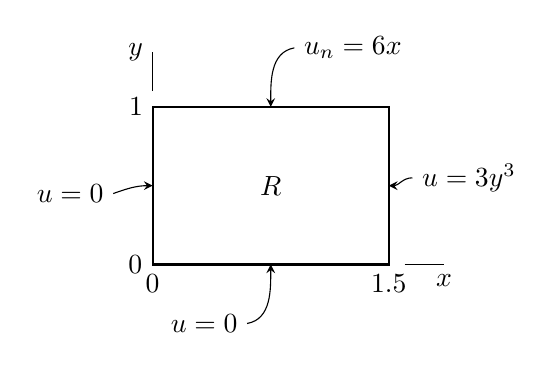
\begin{tikzpicture}
\draw(3.2,0)--++(0.5,0)node[below]{$x$};
\draw(0,2.2)--++(0,0.5)node[left]{$y$};
\draw[thick] (0,0)node[below]{$0$}node[left]{$0$} rectangle (3,2);
\draw(1.5,1)node[]{$R$};
\draw(0,2)node[left]{$1$};
\draw(3,0)node[below]{$1.5$};
\draw[stealth-](1.5,0) to [out=-90,in=10]++(-0.3,-0.75)node[left]{$u=0$};
\draw[stealth-](1.5,2) to [out=90,in=-170]++(0.3,0.75)node[right]{$u_n=6x$};
\draw[stealth-](0,1) to [out=180,in=20] ++(-0.5,-0.1)node[left]{$u=0$};
\draw[stealth-](3,1) to [out=0,in=180]++(0.3,0.1)node[right]{$u=3y^3$};
\end{tikzpicture}
\caption*{(الف) خطہ \عددی{R} اور سرحدی قیمتیں}
\end{subfigure}%
\begin{subfigure}{0.5\textwidth}
\centering
\begin{tikzpicture}
\foreach \x in {0,0.5,1,1.5}{\draw(2*\x,-0.5)node[below,font=\small]{$\x$}--(2*\x,2);}
\foreach \y in {0,0.5,1.0}{\draw(-0.25,2*\y)node[left,font=\small]{$\y$}--(3,2*\y);}
\draw[dashed] (1,2)--++(0,1)node[solid,ocirc]{}node[solid,shift={(0.3,0.2)},font=\small]{$N_{13}$};
\draw[dashed] (2,2)--++(0,1)node[solid,ocirc]{}node[solid,shift={(0.3,0.2)},font=\small]{$N_{23}$};
\draw(0,1)node[ocirc]{}node[shift={(0.3,0.2)},font=\small]{$N_{01}$}node[shift={(0.4,-0.2)},font=\small]{$u=0$};
\draw(0,2)node[ocirc]{}node[shift={(0.3,0.2)},font=\small]{$N_{02}$};
\draw(1,0)node[ocirc]{}node[shift={(0.3,0.2)},font=\small]{$N_{10}$}node[shift={(0.4,-0.2)},font=\small]{$u=0$};
\draw(2,0)node[ocirc]{}node[shift={(0.3,0.2)},font=\small]{$N_{20}$}node[shift={(0.4,-0.2)},font=\small]{$u=0$};
\draw(3,1)node[ocirc]{}node[shift={(0.3,0.2)},font=\small]{$N_{31}$}node[shift={(0.7,-0.2)},font=\small]{$u=0.375$};
\draw(3,2)node[ocirc]{}node[shift={(0.3,0.2)},font=\small]{$N_{32}$}node[shift={(0.4,-0.2)},font=\small]{$u=3$};
\draw(1,1)node[circ]{}node[shift={(0.3,0.2)},font=\small]{$N_{11}$};
\draw(2,1)node[circ]{}node[shift={(0.3,0.2)},font=\small]{$N_{21}$};
\fill[white](1,2) circle (1.5pt);
\draw(1,2)node[kcross]{}node[shift={(0.3,0.2)},font=\small]{$N_{12}$}node[shift={(0.47,-0.2)},font=\small]{$u_n=3$};
\fill[white](2,2) circle (1.5pt);
\draw(2,2)node[kcross]{}node[shift={(0.3,0.2)},font=\small]{$N_{22}$}node[shift={(0.47,-0.2)},font=\small]{$u_n=6$};
\end{tikzpicture}
\caption*{(ب) جال}
\end{subfigure}%
\caption{اشکال برائے مثال \حوالہ{مثال_اعدادی_پوئسن_مخلوط_سرحدی_الف}}
\label{شکل_مثال_اعدادی_پوئسن_مخلوط_سرحدی_الف}
\end{figure}

حل:\quad
ہم شکل \حوالہ{مثال_اعدادی_پوئسن_مخلوط_سرحدی_الف}-ب میں دکھایا گیا جال استعمال کرتے ہیں جہاں \عددی{h=0.5} ہے۔ کلیات \عددی{u=3y^3} اور \عددی{u_n=6x} سے  سرحد پر
\begin{align}\label{مساوات_اعدادی_مخلوط_سرحدی_الف}
u_{31}=0.375,\quad u_{32}=3,\quad \frac{\partial u_{12}}{\partial n}=\frac{\partial u_{12}}{\partial y}=3,\quad \frac{\partial u_{22}}{\partial n}=\frac{\partial u_{22}}{\partial y}=6
\end{align}
حاصل ہو گا۔ \عددی{N_{11}} اور \عددی{N_{21}} خطہ \عددی{R} کے اندرونی نقطے ہیں لہٰذا ان سے گزشتہ حصہ  کی طرح برتا جا سکتا ہے۔ یقیناً \عددی{h^2=0.25}،  \عددی{f(x,y)=12xy} اور سرحدی معلومات استعمال کرتے ہوئے مساوات \حوالہ{مساوات_اعدادی_جزوی_عمومی_ج}  سے \عددی{N_{11}} اور \عددی{N_{21}} کے لئے درج ذیل لکھا جا سکتا ہے۔
\begin{gather}
\text{(الف)}\quad 
\begin{aligned}\label{مساوات_اعدادی_مخلوط_سرحدی_ب}
-4u_{11}+u_{21}+u_{12}\phantom{+u_{21}}&=0.75\\
u_{11}-4u_{21}\phantom{+u_{21}}+u_{22}&=1.5-0.375=1.125
\end{aligned}
\end{gather}
ان مساوات میں سرحد کے نقطہ \عددی{N_{12}} اور \عددی{N_{22}} پر \عددی{u} کی قیمتیں \عددی{u_{12}} اور \عددی{u_{22}} درکار ہیں جبکہ ہمیں ان نقطوں پر عمودی تفرق \عددی{u_n=\tfrac{\partial u}{\partial n}=\tfrac{\partial u}{\partial y}} کی قیمتیں دی گئی ہیں۔ہم اس مشکل سے جلد نجات حاصل کر پائیں گے۔

ہم نقطہ \عددی{N_{13}} اور \عددی{N_{23}} پر غور کرتے ہیں۔ہم تصور میں \عددی{R} کو  وسعت دے کر بالائی جانب پہلی بیرونی صف (یعنی \عددی{y=1.5} کے مطابقتی نقطوں)  کو   \عددی{R} میں شامل کرتے ہیں اور ساتھ ہی فرض کرتے ہیں کہ تفرقی مساوات توسیع کردہ خطہ میں بھی کارآمد ہے۔تب ہم پہلے کی طرح مزید دو مساوات
\begin{equation*}\tag{\ref{مساوات_اعدادی_مخلوط_سرحدی_ب}}
\text{(ب)}\quad
\begin{aligned}
u_{11}\phantom{+u_{21}}-4u_{12}+u_{22}+u_{13}\phantom{+u_{12}}&=1.5\\
u_{21}+u_{12}-4u_{22}\phantom{+u_{12}}+u_{23}&=3-3=0
\end{aligned}
\end{equation*}
لکھ سکتے ہیں (شکل \حوالہ{شکل_مثال_اعدادی_پوئسن_مخلوط_سرحدی_الف}-ب)۔دھیان رہے کہ \عددی{R} کی بالائی سرحد پر دی گئی معلومات کو اب تک ہم نے استعمال نہیں کیا ہے، اور مساوات \حوالہ{مساوات_اعدادی_مخلوط_سرحدی_ب}-ب میں ہم نے دو اضافی متغیرات \عددی{u_{13}} اور \عددی{u_{23}} بھی متعارف کیے ہیں۔اب ہم بالائی سرحد پر دی گئی معلومات اور \عددی{u_y} کی مساوات فرق  استعمال کرتے ہوئے  \عددی{u_{13}} اور \عددی{u_{23}} سے چھٹکارا حاصل کرتے ہیں۔ یوں مساوات \حوالہ{مساوات_اعدادی_مخلوط_سرحدی_الف} سے 
\begin{align*}
3=\frac{\partial u_{12}}{\partial y}&=\frac{u_{13}-u_{11}}{2h}=u_{13}-u_{11}\quad \implies \quad u_{13}=u_{11}+3\\
6=\frac{\partial u_{22}}{\partial y}&=\frac{u_{23}-u_{21}}{2h}=u_{23}-u_{21}\quad \implies \quad u_{23}=u_{21}+6
\end{align*}
حاصل ہو گا جنہیں مساوات \حوالہ{مساوات_اعدادی_مخلوط_سرحدی_ب}-ب میں پر کر کے درج ذیل حاصل ہو گا۔
\begin{align*}
2u_{11}\phantom{+u_{32}}-4u_{12}+u_{22}&=1.5-3=-1.5\\
2u_{21}+u_{12}-4u_{22}&=0-6=-6
\end{align*}
انہیں مساوات \حوالہ{مساوات_اعدادی_مخلوط_سرحدی_ب}-الف کے ساتھ ملا کر قالبی صورت میں لکھتے ہیں۔
\begin{align}\label{مساوات_اعدادی_قالب_الف}
\begin{bmatrix*}[r]
-4&1&1&0\\
1&-4&0&1\\
2&0&-4&1\\
0&2&1&-4
\end{bmatrix*}
\begin{bmatrix}
u_{11}\\
u_{21}\\
u_{12}\\
u_{22}
\end{bmatrix}=
\begin{bmatrix*}[r]
0.750\\
1.125\\
-1.500\\
-6.000
\end{bmatrix*}
\end{align}
اس کا حل درج ذیل ہے جہاں بالکل درست حل کو ساتھ قوسین میں دکھایا گیا ہے۔
\begin{gather*}
\begin{aligned}
u_{12}&=0.866\,\,(1.000)\\
u_{11}&=0.077\,\,(0.125)
\end{aligned}\quad\quad
\begin{aligned}
u_{22}&=1.812\,\,(2.000)\\
u_{21}&=0.191\,\,(0.250)
\end{aligned}
\end{gather*}
\انتہا{مثال}
%=========================

\جزوحصہء{غیر منظم سرحد}
ہم \عددی{xy} مستوی میں خطہ \عددی{R} پر بیضوی مساوات کے سرحدی مسئلے کے اعدادی حل پر غور جاری رکھتے ہیں۔اگر \عددی{R} کی سادہ جیومیٹریائی شکل ہو تب عموماً ہم جال کو یوں بچھا سکتے ہیں کہ \عددی{R} کی سرحد \عددی{C} پر جال کے کئی جوڑ پائے جاتے ہوں۔یوں ہم جزوی تفرق کو گزشتہ حصہ کی طرح تخمینی طور پر لکھ سکتے ہیں۔البتہ اگر سرحد \عددی{C} جال کو جوڑ سے ہٹ کر قطع کرتا ہو تب سرحد کے قریب نقطوں پر ہمیں کچھ مختلف طرز عمل اختیار کرنا ہو گا۔آئیں ایسی صورت کو دیکھیں۔

شکل \حوالہ{شکل_اعدادی_غیر_منظم_سرحد} میں جوڑ \عددی{O} اس قسم کا نقطہ ہے۔ \عددی{O} اور اس کے پڑوسی نقطے \عددی{A} اور \عددی{P} کے لئے ٹیلر تسلسل لکھتے ہیں۔
\begin{gather}
\begin{aligned}\label{مساوات_اعدادی_غیر_ہموار_سرحد_الف}
\text{(الف)}\quad u_A&=u_O+ah\frac{\partial u_O}{\partial x}+\frac{1}{2}(ah)^2\frac{\partial^{\,2}u_O}{\partial x^2}+\cdots\\
\text{(ب)}\quad u_P&=u_O-h\frac{\partial u_O}{\partial x}+\frac{1}{2}h^2\frac{\partial^{\,2}u_O}{\partial x^2}+\cdots
\end{aligned}
\end{gather}
ہم ٹیلر تسلسل کی پہلی تین اجزاء لیتے ہوئے باقی اجزاء  کو رد کرتے ہیں اور ساتھ ہی \عددی{\tfrac{\partial u_O}{\partial x}} کو حذف کرنے کی غرض سے مساوات \حوالہ{مساوات_اعدادی_غیر_ہموار_سرحد_الف}-ب کو \عددی{a} سے ضرب دے کر مساوات \حوالہ{مساوات_اعدادی_غیر_ہموار_سرحد_الف}-الف کے ساتھ جمع کرتے ہوئے
\begin{align*}
u_A+au_P\approx (1+a)u_O+\frac{1}{2}a(1+a)h^2\frac{\partial^{\,2}u_O}{\partial x^2}
\end{align*}
حاصل کرتے ہیں جس سے درج ذیل لکھا جا سکتا ہے۔
\begin{align*}
\frac{\partial^{\,2}u_O}{\partial x^2}\approx \frac{2}{h^2}\left[\frac{1}{a(1+a)}u_A+\frac{1}{1+a}u_P-\frac{1}{a}u_O\right]
\end{align*}
اسی طرح نقطہ \عددی{O}، \عددی{B} اور \عددی{Q} کے لئے درج ذیل لکھا جا سکتا ہے۔
\begin{align*}
\frac{\partial^{\,2}u_O}{\partial y^2}\approx \frac{2}{h^2}\left[\frac{1}{b(1+b)}u_B+\frac{1}{1+b}u_Q-\frac{1}{b}u_O\right]
\end{align*}
درج بالا دونوں مساوات کا مجموعہ
\begin{align}\label{مساوات_اعدادی_نیبلا_الف}
\nabla^{\,2}u_O\approx \frac{2}{h^2}\left[\frac{u_A}{a(1+a)}+\frac{u_B}{b(1+b)}+\frac{u_P}{1+a}+\frac{u_Q}{1+b}-\frac{(a+b)u_O}{ab}\right]
\end{align}
ہو گا۔مثال کے طور پر اگر \عددی{a=\tfrac{1}{2}}، \عددی{b=\tfrac{1}{2}} ہوں تب مساوات \حوالہ{مساوات_اعدادی_جزوی_عمومی_ح} کی نقش کی بجائے درج ذیل نقش 
\begin{align*}
\left \{ 
\begin{matrix*}[r]
&\frac{4}{3}&\\
\frac{2}{3}&-4&\phantom{-}\frac{4}{3}\\
&\frac{2}{3}&
\end{matrix*}
\right\}
\end{align*}
حاصل ہو گا۔اس نقش کے پانچ اعداد کا مجموعہ اب بھی صفر کے برابر ہے (جو درستگی کو پرکھنے کی ایک اچھی ترکیب ہے)۔
\begin{figure}
\centering
\begin{minipage}{0.45\textwidth}
\centering
\begin{tikzpicture}
\foreach \x in {0,1,2}{\draw(\x,-0.25)--++(0,2.5);}
\foreach \y in {0,1,2}{\draw(-0.25,\y)--++(2.5,0);}
\draw(1,0)node[ocirc]{}node[shift={(0.2,0.2)},font=\small]{$Q$};
\draw(1,1)node[circ]{}node[shift={(0.2,0.2)},font=\small]{$O$};
\draw(0,1)node[ocirc]{}node[shift={(0.2,0.2)},font=\small]{$P$};
\draw[thick,name path=C] (0.25,2.25) to [out=-20,in=135] (2.25,0.5)node[right]{$C$};
\path[name path=A](1,0)--++(0,2.25);
\path[name path=B](0,1)--++(2.25,0);
\draw[name intersections={of=A and C}] (intersection-1)node[ocirc]{}node[right,font=\small]{$B$};
\draw(intersection-1)++(-0.1,0)--++(-0.4,0)coordinate[pos=0.5](kU);
\draw[stealth-stealth](kU)--($(0,1)!(kU)!(2,1)$)node[pos=0.5,fill=white,font=\small]{$bh$};
\draw[name intersections={of=B and C}] (intersection-1)node[ocirc]{}node[shift={(0.1,0.2)},font=\small]{$A$};
\draw(intersection-1)++(0,-0.1)--++(0,-0.4)coordinate[pos=0.5](kR);
\draw[stealth-stealth](kR)--($(1,0)!(kR)!(1,2)$)node[pos=0.5,fill=white,font=\small]{$ah$};
\draw[stealth-stealth] (0,0.4)--++(1,0)node[pos=0.5,fill=white]{$h$};
\end{tikzpicture}
\caption{غیر منظم سرحد}
\label{شکل_اعدادی_غیر_منظم_سرحد}
\end{minipage}\hfill
\begin{minipage}{0.45\textwidth}
\centering
\begin{tikzpicture}
\draw(0,0)node[ocirc]{}node[left,font=\small]{$P$}--++(2,0)node[ocirc]{}node[right,font=\small]{$A$};
\draw(1,-1)node[ocirc]{}node[right,font=\small]{$Q$}--++(0,2)node[ocirc]{}node[right,font=\small]{$B$};
\draw(1,0)node[circ]{}node[shift={(0.2,0.2)},font=\small]{$O$};
\draw(0.5,0)node[below]{$ph$};
\draw(1.5,0)node[below]{$ah$};
\draw(1,0.5)node[left]{$bh$};
\draw(1,-0.6)node[left]{$qh$};
\end{tikzpicture}
\caption{جوڑ \عددی{O} کے پڑوسی نقطے \عددی{A}، \عددی{B}، \عددی{P} اور \عددی{Q}}
\label{شکل_اعدادی_جوڑ_کے_پڑوسی_نقطے}
\end{minipage}%
\end{figure}

اسی طرح آپ شکل \حوالہ{شکل_اعدادی_جوڑ_کے_پڑوسی_نقطے} کے لئے 
\begin{align}\label{مساوات_اعدادی_نیبلا_ب}
\nabla^{\,2}u_O\approx \frac{2}{h^2}\left[\frac{u_A}{a(a+p)}+\frac{u_B}{b(b+q)}+\frac{u_P}{p(p+a)}+\frac{u_Q}{q(q+b)}-\frac{ap+bq}{abpq}u_O\right]
\end{align}
حاصل کر سکتے ہیں جو ہر ممکنہ صورت حاصل کو نپٹا سکتی ہے۔

%==================
\ابتدا{مثال}\شناخت{مثال_اعدادی_غیر_منظم_سرحد_ڈرشلے}\quad \موٹا{مساوات لاپلاس کا مسئلہ ڈرشلے۔ قوسی سرحد}\\
شکل \حوالہ{شکل_مثال_اعدادی_غیر_منظم_سرحد_ڈرشلے} میں دکھائے گئے خطہ میں مخفی قوہ \عددی{u} تلاش کریں۔یہاں سرحد کو قوسی حصہ ایک دائرے کا حصے ہے جس کا رداس \عددی{10} اور مرکز \عددی{(0,0)} ہے۔سرحدی معلومات شکل میں دی گئیں ہیں۔شکل میں دیا گیا جال استعمال کریں۔
\begin{figure}
\centering
\begin{tikzpicture}[x=0.4cm,y=0.4cm]
\pgfmathsetmacro{\angS}{atan(6/8)}
\pgfmathsetmacro{\angE}{asin(9/10)}
\draw(8.3,0)--++(2,0)node[right]{$x$};
\draw(0,9.3)--++(0,1)node[left]{$y$};
\draw[name path=kC,thick]([shift={(\angS:10)}]0,0) arc (\angS:\angE:10)-|(0,0)node[left]{$0$}node[below]{$0$}--(8,0)--cycle;
\draw(3,0)node[ocirc]{}node[below]{$3$}node[above right,font=\small]{$u=27$}--++(0,9)node[ocirc]{}node[above right]{$u=-702$};
\path[name path=kV] (6,0)--++(0,9);
\draw[name intersections={of=kV and kC}](intersection-1)node[ocirc]{}node[right]{$u=-936$}--(6,0)node[ocirc]{}node[below]{$6$}node[shift={(0.3cm,0.3cm)},font=\small]{$\substack{u=\\216}$};
\foreach \y/\kt in {3/1,6/2}{\draw(0,\y)node[left]{$\y$}node[ocirc]{}--++(8,0)node[ocirc]{} (3,\y)node[ocirc]{}node[shift={(0.8,0.5)},font=\small]{$N_{1\kt}$} (6,\y)node[ocirc]{}node[shift={(0.8,0.5)},font=\small]{$N_{2\kt}$};}
\draw(0,9)node[left]{$9$};
\draw(8,3)node[right]{$u=296$};
\draw(0,3)node[above right]{$u=0$};
\draw(0,6)node[above right]{$u=0$};
\draw(8,6)node[right]{$u=-352$};
\draw[stealth-] (0,4.5) to [out=180,in=20]++(-3,-2)node[left]{$u=0$};
\draw[stealth-] (5,0) to [out=-90,in=20]++(-3,-2)node[left]{$u=x^3$};
\draw[stealth-] (8,4) to [out=30,in=180]++(3,1)node[right]{$u=512-24y^2$};
\draw[stealth-] (1,9) to [out=60,in=180]++(3,2)node[right]{$u=x^3-243x$};
\end{tikzpicture}
\caption{شکل برائے مثال \حوالہ{مثال_اعدادی_غیر_منظم_سرحد_ڈرشلے}}
\label{شکل_مثال_اعدادی_غیر_منظم_سرحد_ڈرشلے}
\end{figure} 

حل:\quad
مساوات لاپلاس کا حل \عددی{u} ہو گا۔سرحد پر کلیات \عددی{u=x^3}، \عددی{u=512-24y^2}، وغیرہ سے ہم درکار نقطوں پر قیمتیں حاصل کرتے ہیں جنہیں شکل میں دکھایا گیا ہے۔\عددی{N_{11}} اور \عددی{N_{12}} کے لئے  عمومی منظم نقش حاصل ہوتا ہے، اور \عددی{N_{21}} اور \عددی{N_{22}} کے لئے ہم مساوات \حوالہ{مساوات_اعدادی_نیبلا_ب} سے
\begin{align}\label{مساوات_اعدادی_مثال_لاپلاس_ڈرشلے}
N_{11}, \, N_{12}:
\left\{ 
\begin{matrix*}[r]
&1&\\
1&-4&\phantom{-}1\\
&1&
\end{matrix*}
 \right\},\,\,
N_{21}:\left\{
\begin{matrix*}[r]
&0.5&\\
0.6&-2.5&0.9\\
&0.5&
\end{matrix*}
\right\},\,\,
N_{22}:\left\{
\begin{matrix*}[r]
&0.9&\\
0.6&-3.0&0.9\\
&0.6&
\end{matrix*}
\right\}
\end{align}
حاصل کرتے ہیں۔ہم  انہیں اور سرحدی قیمتیں  کو استعمال کرتے ہیں اور جوڑوں  کو \عددی{N_{11}}، \عددی{N_{21}}، \عددی{N_{12}}، \عددی{N_{22}} ترتیب میں  لیتے ہیں۔یوں درج ذیل نظام حاصل ہوتا ہے۔
\begin{gather*}
\begin{aligned}
-4u_{11}+u_{21}+u_{12}\phantom{+u_{32}}&=0-27\\
0.6u_{11}-2.5u_{21}\phantom{u_{32}}+0.5u_{22}&=-0.9(296)-0.5(216)\\
u_{11}\phantom{+u_{32}}-4u_{12}+u_{22}&=702+0\\
0.6u_{21}+0.6u_{12}-3u_{22}&=0.9(352)+0.9(936)
\end{aligned}
\begin{aligned}
&=-27\\
&=-374.4\\
&=\phantom{-}702\\
&=\phantom{-}1159.2
\end{aligned}
\end{gather*}
اس کو قالبی صورت میں لکھ کر
\begin{align}\label{مساوات_اعدادی_مثال_لاپلاس_ڈرشلے_ب}
\begin{bmatrix}
-4&1&1&0\\
0.6&-2.5&0&0.5\\
1&0&-4&1\\
0&0.6&0.6&-3
\end{bmatrix}
\begin{bmatrix}
u_{11}\\
u_{21}\\
u_{12}\\
u_{22}
\end{bmatrix}=
\begin{bmatrix}
-27\\
-374.4\\
702\\
1159.2
\end{bmatrix}
\end{align}
گاوسی اسقاط کی مدد سے درج ذیل نتائج حاصل کرتے ہیں۔
\begin{align*}
u_{11}=-55.6,\quad u_{21}=49.2,\quad u_{12}=-298.5,\quad u_{22}=-436.3
\end{align*}
ظاہر ہے کہ اتنے کم خانوں کی جال سے ہمیں زیادہ درست نتائج حاصل نہیں ہوں گے۔بالکل درست نتائج درج ذیل ہیں۔
\begin{align*}
u_{11}=-54,\quad u_{21}=54,\quad u_{12}=-297,\quad u_{22}=-432
\end{align*}
عملاً بہت باریک جال استعمال کرتے ہوئے بڑا نظام حاصل کیا جائے گا جس کو بالواسطہ ترکیب سے حل کیا جائے گا۔
\انتہا{مثال}
%====================

\حصہء{سوالات}
%==========================
\ابتدا{سوال}\quad 
مساوات \حوالہ{مساوات_اعدادی_قالب_الف} کے نظام کو گاوسی اسقاط سے حل کرتے ہوئے مثال \حوالہ{مثال_اعدادی_پوئسن_مخلوط_سرحدی_الف} کی آخر میں دی گئی قیمتوں کو پرکھیں۔
\انتہا{سوال}
%===========================
\ابتدا{سوال}\quad
شکل \حوالہ{شکل_مثال_اعدادی_پوئسن_مخلوط_سرحدی_الف}-الف کی مستطیل میں  (اور شکل-ب کا جال استعمال کرتے ہوئے) مساوات لاپلاس \عددی{\nabla^{\,2}u=0} کا ابتدائی قیمت مسئلہ حل کریں جہاں بائیں چادر پر \عددی{u_x=0}، دائیں چادر پر \عددی{u_x=3}، نچلی چادر پر \عددی{u=x^2} اور بالائی چادر پر \عددی{u=x^2-1} ہیں۔
\انتہا{سوال}
%===========================
\ابتدا{سوال}\شناخت{سوال_اعدادی_مخلوط_الف}\quad
مساوات پوئسن \عددی{\nabla^{\,2}u=2(x^2+y^2)} کے مخلوط قیمت مسئلے کا حل شکل \حوالہ{شکل_سوال_اعدادی_مخلوط_الف} کے لئے  (شکل میں دیے گئے جال کے لئے) حاصل کریں۔سرحدی معلومات شکل میں دی گئی ہیں۔
\begin{figure}
\centering
\begin{minipage}{0.45\textwidth}
\centering
\begin{tikzpicture}
\draw (3.2,0)--++(0.5,0)node[right]{$x$};
\draw(0,3.2)--++(0,0.5)node[left]{$y$};
\draw[thick] (0,0)node[left]{$0$}node[below]{$0$} rectangle (3,3);
\foreach \x in {1,2} {\draw(\x,0)node[below]{$\x$}--++(0,3);}
\foreach \y in {1,2}{\draw(0,\y)node[left]{$\y$}--++(3,0)  (1,\y)node[ocirc]{}node[shift={(0.3,0.2)},font=\small]{$N_{1\y}$}   (2,\y)node[ocirc]{}node[shift={(0.3,0.2)},font=\small]{$N_{2\y}$};}
\draw[stealth-] (1.5,0) to [out=-90,in=0]++(-0.3,-0.75) node[left]{$u=0$};
\draw[stealth-] (1.5,3) to [out=90,in=180]++(0.3,0.5) node[right]{$u=9x^2$};
\draw[stealth-] (0,1.5) to [out=-135,in=30]++(-0.3,-0.3) node[left]{$u=0$};
\draw[stealth-] (3,1.5) to [out=20,in=180]++(0.3,0.3) node[right]{$u=6y^2$};
\end{tikzpicture}
\caption{شکل برائے سوال \حوالہ{سوال_اعدادی_مخلوط_الف}}
\label{شکل_سوال_اعدادی_مخلوط_الف}
\end{minipage}\hfill
\begin{minipage}{0.45\textwidth}
\centering
\begin{tikzpicture}
\draw (3.2,0)--++(0.5,0)node[right]{$x$};
\draw(0,3.2)--++(0,0.5)node[left]{$y$};
\draw[thick,name path=kC] (0,0)node[left]{$0$}node[below]{$0$}--++(3,0)--++(0,1.5)--++(-1.5,1.5)--++(-1.5,0)--++(0,-3);
\draw(1,0)--++(0,3);
\draw(0,1)--++(3,0);
\draw(2,0)--++(0,2.5);
\draw(0,2)--++(2.5,0);
\draw(1,1)node[ocirc]{}node[shift={(0.3,-0.2)}]{$N_{11}$}  (2,1)node[ocirc]{}node[shift={(0.3,-0.2)}]{$N_{21}$}  (1,2)node[ocirc]{}node[shift={(0.3,-0.2)}]{$N_{12}$}  (2,2)node[ocirc]{}node[shift={(0.3,-0.2)}]{$N_{22}$};
\draw[stealth-] (1.5,0) to [out=-90,in=0]++(-0.3,-0.75) node[left]{$u=3x$};
\draw[stealth-] (0.5,3) to [out=90,in=180]++(0.3,0.5) node[right]{$u=0$};
\draw[stealth-] (0,1.5) to [out=-135,in=30]++(-0.3,-0.3) node[left]{$u=0$};
\draw[stealth-] (3,0.5) to [out=20,in=180]++(0.3,0.3) node[right]{$u=9-3y$};
\draw[stealth-] (2.2,2.3) to [out=20,in=180]++(0.3,0.3) node[right]{$u=x^2-1.5x$};
\end{tikzpicture}
\caption{شکل برائے سوال \حوالہ{سوال_اعدادی_مخلوط_ب}}
\label{شکل_سوال_اعدادی_مخلوط_ب}
\end{minipage}
\end{figure}
 

جواب:\quad
$u_{11}=1,\,\,u_{21}=u_{12}=4,\,\,u_{22}=16$
\انتہا{سوال}
%========================
\ابتدا{سوال}\quad
مساوات \حوالہ{مساوات_اعدادی_غیر_ہموار_سرحد_الف} میں سے \عددی{\tfrac{\partial^{\,2}u_O}{\partial x^2}} حذف کرتے ہوئے درج ذیل حاصل کریں۔
\begin{align*}
\tfrac{\partial u_O}{\partial x}\approx \tfrac{1}{h}[\tfrac{1}{a(1+a)}u_A-\tfrac{1-a}{a}u_O-\tfrac{a}{1+a}u_P]
\end{align*}
\انتہا{سوال}
%===========================
\ابتدا{سوال}\quad
ٹھیک مساوات \حوالہ{مساوات_اعدادی_نیبلا_الف} کے  بعد دی گئی نمونہ حساب کی تصدیق کریں۔
\انتہا{سوال}
%========================
\ابتدا{سوال}\quad
مساوات \حوالہ{مساوات_اعدادی_نیبلا_ب}  حاصل کرنے کی تفصیل پیش کریں۔
\انتہا{سوال}
%===========================
\ابتدا{سوال}\quad
مساوات \حوالہ{مساوات_اعدادی_مثال_لاپلاس_ڈرشلے} کی تصدیق کریں۔
\انتہا{سوال}
%=========================
\ابتدا{سوال}\quad
قالبی مساوات \حوالہ{مساوات_اعدادی_مثال_لاپلاس_ڈرشلے_ب} کو گاوسی اسقاط کی مدد سے حل کریں۔
\انتہا{سوال}
%===========================
\ابتدا{سوال}\شناخت{سوال_اعدادی_مخلوط_ب}\quad
مساوات لاپلاس  کا حل شکل \حوالہ{شکل_سوال_اعدادی_مخلوط_ب} میں دیے گئے مسئلہ کے لئے  (شکل میں دیے گئے جال پر) حاصل کریں۔سرحدی معلومات شکل میں دی گئی ہیں۔(سرحد کا ترچھا حصہ \عددی{y=4.5-x} ہے۔)\\
جواب:\quad
$-4u_{11}+u_{21}+u_{12}=-3,\,\, u_{11}-4u_{21}+u_{22}=-12,\,\, u_{11}-4u_{12}+u_{22}=0,$\\
$2u_{21}+2u_{12}-12u_{22}=-14,\,\, u_{11}=u_{22}=2,\,\, u_{21}=4,\,\, u_{12}=1$
\انتہا{سوال}
%========================
\ابتدا{سوال}\شناخت{سوال_اعدادی_پوئسن_دو}\quad
مساوات پوئسن \عددی{\nabla^{\,2}u=2} کو شکل \حوالہ{شکل_سوال_اعدادی_پوئسن_دو} کے خطہ کے لئے حل کریں۔
\begin{figure}
\centering
\begin{tikzpicture}
\draw(3.2,0)--++(0.5,0)node[right]{$x$};
\draw(0,3.2)--++(0,0.5)node[left]{$y$};
\draw[thick,name path=kCur] (0,0)node[left]{$0$}node[below]{$0$}--(3,0)node[below]{$3$}--(3,1.5)--(0,3)node[left]{$3$}--(0,0);
\path[name path=kA] (1,0)--++(0,3);
\path[name path=kB] (2,0)--++(0,3);
\path[name path=kC] (0,1)--++(3,0);
\path[name path=kD] (0,2)--++(3,0);
\draw[name intersections={of={kCur and kA}}] (intersection-1)--(intersection-2);
\draw[name intersections={of={kCur and kB}}] (intersection-1)--(intersection-2);
\draw[name intersections={of={kCur and kC}}] (intersection-1)--(intersection-2);
\draw[name intersections={of={kCur and kD}}] (intersection-1)--(intersection-2);
\draw (1,1)node[ocirc]{}node[shift={(-0.3,-0.2)}]{$N_{11}$}  (2,1)node[ocirc]{}node[shift={(-0.3,-0.2)}]{$N_{21}$}  (1,2)node[ocirc]{}node[shift={(-0.3,-0.2)}]{$N_{12}$};
\draw (1,0)node[below]{$1$} (2,0)node[below]{$2$} (0,1)node[left]{$1$} (0,2) node[left]{$2$};
\draw[stealth-] (0,1.5) to [out=180,in=0]++(-0.3,-0.2)node[left]{$u=y^2-3y$};
\draw[stealth-] (3,0.5) to [out=0,in=180]++(0.3,0.2)node[right]{$u=y^2-1.5y$};
\draw[stealth-] (1.5,0) to [out=-90,in=0]++(-0.3,-0.75)node[left]{$u=0$};
\draw[stealth-] ($(3,1.5)!0.5!(0,3)$) to [out=45,in=180]++(0.3,0.2)node[right]{$u=0$};
\end{tikzpicture}
\caption{شکل برائے سوال \حوالہ{سوال_اعدادی_پوئسن_دو}}
\label{شکل_سوال_اعدادی_پوئسن_دو}
\end{figure}
\انتہا{سوال}
%==========================

\حصہ{اعدادی تراکیب برائے قطع مکافی مساوات}
جیسا کہ ہم نے حصہ \حوالہ{حصہ_اعدادی_بیضوی_مساوات} میں ذکر کیا، مختلف اقسام کی مساوات مثلاً بیضوی، قطع مکافی اور قطع زائد کے حل کا رویہ مختلف ہو گا۔اسی طرح ان کے اعدادی تراکیب بھی کچھ مختلف ہوں گے۔تینوں اقسام میں ہم مساوات کی جگہ  مطابقتی مساوات فرق لکھتے ہیں لیکن \ترچھا{قطع مکافی} اور \ترچھا{قطع زائد} مساوات کی صورت میں ضروری نہیں ہے کہ تخمینی اعدادی حل، \عددی{h\to 0} کرنے سے، اصل حل کو مرتکز  ہو، بلکہ اس سے  کسی صورت بھی ارتکاز یقینی نہیں ہو گا۔ان دو صورتوں میں مرتکز (اور \اصطلاح{مستحکم}) حل  کے لئے  اضافی شرائط (عدم مساوات) کا ہونا  لازمی ہے۔حل کی استحکام سے مراد یہ ہے کہ ابتدائی معلومات میں معمولی اضطراب (یا کسی بھی لمحہ پر معمولی اضطراب) بعد میں بھی معمولی ہی رہے گی۔ 

اس حصہ میں ہم حراری مساوات کو مثال بناتے ہوئے  قطع مکافی مساوات کے اعدادی حل پر غور کرتے ہیں۔ہم مذکورہ بالا  اور دیگر صورتوں پر یک بعدی حراری مساوات
\begin{align*}
u_t=c^2u_{xx}\quad \quad \quad (\text{مستقل}\,\, c)
\end{align*}
کی مدد سے غور کرتے ہیں۔ اس مساوات پر عموماً کسی وقفہ \عددی{0\le x\le l} میں وقت \عددی{t\ge 0} کے لئے غور کیا جاتا ہے جہاں ابتدائی درجہ حرارت \عددی{u(x,0)=f(x)} (جہاں \عددی{f} دیا گیا ہو گا) اور تمام \عددی{t\ge 0} کے لئے \عددی{x=0} اور \عددی{x=l} پر سرحدی معلومات، مثلاً \عددی{u(0,t)=0,\, u(l,t)=0}، دی گئی ہوں گی۔ ہم اپنی آسانی کی خاطر \عددی{c=1} اور \عددی{l=1} لیتے ہیں جو \عددی{x} اور \عددی{t} کی خطی تبادل سے ممکن ہو گا (سوال \حوالہ{سوال_اعدادی_غیر_بعدی_معیاری_حراری_مساوات})۔تب حراری مساوات اور دی گئی معلومات درج ذیل ہوں گی۔
\begin{align}
u_t&=u_{xx}\quad \quad 0\le x\le l,\, t\ge 0  \label{مساوات_اعدادی_حراری_الف}\\
u(x,0)&=f\quad \quad\quad  (\text{\RL{ابتدائی شرائط}}) \label{مساوات_اعدادی_حراری_ب}\\
u(0,t)&=u(l,t)=0\quad (\text{\RL{سرحدی شرائط}}) \label{مساوات_اعدادی_حراری_پ}
\end{align}

مساوات \حوالہ{مساوات_اعدادی_حراری_الف} کا مطابقتی تخمینی مساوات فرق درج ذیل ہے۔
\begin{align}\label{مساوات_اعدادی_حراری_ت}
\frac{1}{k}(u_{i,j+1}-u_{ij})=\frac{1}{h^2}(u_{i+1,j}-2u_{ij}+u_{i-1,j})
\end{align}
شکل \حوالہ{شکل_اعدادی_حراری_قطع_مکافی_غور} میں مطابقتی جال اور جوڑ دکھائے گئے ہیں۔\عددی{x} رخ میں جسامت جال \عددی{h} ہے جبکہ \عددی{t} رخ جسامت جال \عددی{k} ہے۔مساوات \حوالہ{مساوات_اعدادی_حراری_ت} میں استعمال ہونے والے چار نقطوں کو شکل \حوالہ{شکل_اعدادی_حراری_قطع_مکافی_غور_ب} میں دکھایا گیا ہے۔چونکہ منفی  \عددی{t} کے لئے ہمارے پاس کوئی معلومات نہیں ہے لہٰذا بائیں ہاتھ آگے فرق کا حاصل تقسیم استعمال کیا گیا ہے۔مساوات \حوالہ{مساوات_اعدادی_حراری_ت} سے ہم وقت \عددی{t} کی  صف \عددی{j+1} کے لئے \عددی{u_{i,j+1}} کو وقت \عددی{j} کے مطابقتی \عددی{u} کی صورت میں حاصل کرتے ہیں؛ مساوات \حوالہ{مساوات_اعدادی_حراری_ت} کو \عددی{u_{i,j+1}} کے لئے حل کرتے  ہوئے درج ذیل حاصل ہو گا۔
\begin{align}\label{مساوات_اعدادی_حراری_ٹ}
u_{i,j+1}=(1-2r)u_{ij}+r(u_{i+1,j}+u_{i-1,j}),\quad r=\frac{k}{h^2}
\end{align}
 
\begin{figure}
\centering
\begin{minipage}{0.6\textwidth}
\begin{tikzpicture}[y=0.75cm]
\draw(0,3.7)--++(0,0.5)node[left]{$t$};
\draw(4.2,0)--++(0.5,0)node[right]{$x$};
\draw[thick] (0,3.5)--(0,0)node[left]{$0$}node[below]{$0$}--(4,0)node[below]{$1$}--(4,3.5);
\foreach \x in {1,2,3} (\draw(\x,0)--++(0,3.5);)
\foreach \y in {1,2,3}{\draw(0,\y)--++(4,0)node[right]{$(j=\y)$} (1,\y)node[ocirc]{}(2,\y)node[ocirc]{}(3,\y)node[ocirc]{};}
\draw(1,0)node[below]{$h$};
\draw(0,1)node[left]{$k$};
\draw[stealth-](0,1.5) to [out=180,in=0]++(-0.3,0.2)node[left]{$u=0$};
\draw[stealth-](4,1.5) to [out=0,in=180]++(1,0.1)node[right]{$u=0$};
\draw[stealth-](2.5,0) to [out=-90,in=0]++(-0.3,-1)node[left]{$u=f(x)$};
\end{tikzpicture}
\caption{جال اور جوڑ برائے مساوات \حوالہ{مساوات_اعدادی_حراری_ت} اور مساوات \حوالہ{مساوات_اعدادی_حراری_ٹ}}
\label{شکل_اعدادی_حراری_قطع_مکافی_غور}
\end{minipage}\hfill
\begin{minipage}{0.3\textwidth}
\centering
\begin{tikzpicture}
\draw(0,0)--(2,0);
\draw(1,0)--(1,0.75);
\fill[white](0,0) circle (1.5pt);
\fill[white](1,0) circle (1.5pt);
\fill[white](2,0) circle (1.5pt);
\fill[white](0,0.75) circle (1.5pt);
\draw(0,0) node[kcross]{};
\draw(1,0) node[kcross]{};
\draw(2,0) node[kcross]{};
\draw(1,0.75) node[kcross]{};
\draw(0.5,0)node[below]{$h$};
\draw(1.5,0)node[below]{$h$};
\draw(1,0.375)node[left]{$k$};
\end{tikzpicture}
\caption{مساوات \حوالہ{مساوات_اعدادی_حراری_ت} اور مساوات \حوالہ{مساوات_اعدادی_حراری_ٹ} کے چار نقطے}
\label{شکل_اعدادی_حراری_قطع_مکافی_غور_ب}
\end{minipage}
\end{figure}

اس کلیہ سے با آسانی نتائج حاصل ہوں گے البتہ ارتکاز کے لئے ضروری ہے کہ  درج ذیل شرط
\begin{align}\label{مساوات_اعدادی_حراری_ث}
r=\frac{k}{h^2}\le \frac{1}{2}
\end{align}
مطمئن ہو جس سے مساوات \حوالہ{مساوات_اعدادی_حراری_ٹ} میں \عددی{u_{ij}} کا عددی سر غیر منفی ہو گا۔مساوات \حوالہ{مساوات_اعدادی_حراری_ث} کہتی ہے کہ \عددی{t} رخ میں زیادہ تیزی سے نہ چلا جائے۔نیچے ایک مثال دی گئی ہے۔

\جزوحصہء{ترکیب کرینک نکلسن\حاشیہد{فرانسیسی ماہر طبیعیات جان کرینک [1916-2006] اور برطانوی ریاضی دان فلس نکلسن [1917-1968]}}
عملی استعمال میں مساوات \حوالہ{مساوات_اعدادی_حراری_ث} کی شرط مسائل پیدا کرتی ہے۔یقیناً زیادہ درست نتائج کے لئے \عددی{h} کی قیمت کم رکھنا ضروری ہے جس کی بنا  مساوات \حوالہ{مساوات_اعدادی_حراری_ث} کے تحت \عددی{k} بہت کم ہو گا۔مثلاً \عددی{h=0.1} کی صورت میں \عددی{k\le 0.005} ہو گا۔اب \عددی{h} کی قیمت آدھی کرنے  سے، کسی بھی \عددی{t} تک پہنچنے کی خاطر، قدموں کی تعداد چار گنا بڑھتی ہے لہٰذا ہمیں بہتر ترکیب کی ضرورت ہے۔

\عددی{r=\tfrac{k}{h^2}} کی قیمت پر \اصطلاح{ترکیب کرینک نکلسن}\فرہنگ{ترکیب!کرینک نکلسن}\حاشیہب{Crank-Nicolson method}\فرہنگ{method!Crank-Nicolson}  کوئی پابندی عائد نہیں کرتی ہے۔یہ ترکیب شکل \حوالہ{شکل_اعدادی_ترکیب_کرینک_نکلسن} کے چھ نقطوں کو استعمال کرتی ہے۔اس ترکیب میں مساوات \حوالہ{مساوات_اعدادی_حراری_ت} کے دائیں ہاتھ فرق کے حاصل تقسیم کی جگہ شکل \حوالہ{شکل_اعدادی_ترکیب_کرینک_نکلسن} کے دو عدد صف  وقت کے مجموعہ کا \عددی{\tfrac{1}{2}} گنا  پر کیا جاتا ہے۔یوں مساوات \حوالہ{مساوات_اعدادی_حراری_ت} کی بجائے
\begin{multline}
\frac{1}{k}(u_{i,j+1}-u_{ij})=\frac{1}{2h^2}(u_{i+1,j}-2u_{ij}+u_{i-1,j})\\
+\frac{1}{2h^2}(u_{i+1,j+1}-2u_{i,j+1}+u_{i-1,j+1})
\end{multline}
حاصل ہو گا۔دونوں اطراف کو \عددی{2k} سے ضرب دے کر \عددی{r=\tfrac{k}{h^2}} لکھتے ہوئے بائیں ہاتھ صف وقت \عددی{j+1} کے مطابقتی تین اجزاء اور دائیں ہاتھ صف وقت \عددی{j} کے تین مطابقتی اجزاء منتقل کرتے ہوئے
\begin{align}\label{مساوات_اعدادی_کرینک_نکلسن_الف}
(2+2r)u_{i,j+1}-r(u_{i+1,j+1}+u_{i-1,j+1})=(2-2r)u_{ij}+r(u_{i+1,j}+u_{i-1,j})
\end{align}
حاصل ہو گا۔عموماً مساوات \حوالہ{مساوات_اعدادی_کرینک_نکلسن_الف} میں بائیں ہاتھ تینوں اجزاء نا معلوم ہوں گے جبکہ دائیں ہاتھ تینوں اجزاء معلوم ہوں گے۔مساوات \حوالہ{مساوات_اعدادی_حراری_الف} کے وقفہ \عددی{0\le x\le 1} کو \عددی{n} عدد برابر ٹکڑوں میں تقسیم کرنے سے فی صف وقت ہمیں \عددی{n-1} اندرونی جوڑ حاصل ہوں گے (شکل \حوالہ{شکل_اعدادی_حراری_قطع_مکافی_غور} دیکھیں جہاں \عددی{n=4} ہے)۔تب \عددی{j=0} اور \عددی{i=1,\cdots,n-1} کے لئے  مساوات \حوالہ{مساوات_اعدادی_کرینک_نکلسن_الف} سے \عددی{n-1}  عدد خطی مساوات کا نظام  حاصل ہو گا جو پہلی صف وقت کے \عددی{n-1} عدد نا معلوم متغیرات \عددی{u_{11}, u_{21},\cdots, u_{n-1,1}} کو  ابتدائی قیمتوں \عددی{u_{00}, u_{10},\cdots,u_{n0}} اور سرحدی قیمتوں \عددی{u_{01},u_{n1}\, (=0)} کی صورت میں پیش کرتا ہے۔ اسی طرح ہر صف وقت، مثلاً \عددی{j=1}، \عددی{j=2} وغیرہ، کے لئے بھی مساوات \حوالہ{مساوات_اعدادی_کرینک_نکلسن_الف} سے  \عددی{n-1} عدد خطی مساوات کا نظام حاصل کر کے   حل کیا جائے گا۔ 
\begin{figure}
\centering
\begin{tikzpicture}
\draw(0,0)--(2,0);
\draw(0,0.75)--(2,0.75);
\draw(1,0)--(1,0.75);
\draw(0.5,0)node[below]{$h$};
\draw(1.5,0)node[below]{$h$};
\draw(1,0.375)node[right]{$k$};
\foreach \x in {0,1,2}{\fill[white](\x,0) circle (1.5pt);}
\foreach \x in {0,1,2}{\fill[white](\x,0.75) circle (1.5pt);}
\foreach \x in {0,1,2}{\draw(\x,0) node[kcross]{};}
\foreach \x in {0,1,2}{\draw(\x,0.75) node[kcross]{};}
\draw(-1,0)node[left]{\RL{صف وقت \عددی{j}}};
\draw(-1,0.75)node[left]{\RL{صف وقت \عددی{j+1}}};
\end{tikzpicture}
\caption{ترکیب کرینک نکلسن میں استعمال ہونے والے چھ نقطے}
\label{شکل_اعدادی_ترکیب_کرینک_نکلسن}
\end{figure}

اگرچہ \عددی{r=\tfrac{k}{h^2}} پر اب  کوئی پابندی عائد نہیں ہے  البتہ \عددی{h} کی چھوٹی قیمت اب بھی  زیادہ درست نتائج دے گی۔عملاً \عددی{k} کی قیمت یوں منتخب کی جاتی ہے کہ، \عددی{r} کی قیمت بہت زیادہ بڑھائے بغیر، کام میں نمایاں کمی واقع ہو۔مثال کے طور پر عموماً \عددی{r=1} منتخب کرنا بہتر ثابت ہوتا ہے (جو گزشتہ بلا واسطہ ترکیب میں نا ممکن ہو گا)۔تب مساوات \حوالہ{مساوات_اعدادی_کرینک_نکلسن_الف} درج ذیل سادہ صورت اختیار کرتی ہے۔
\begin{align}\label{مساوات_اعدادی_کرینک_نکلسن_ب}
4u_{i,j+1}-u_{i+1,j+1}-u_{i-1,j+1}=u_{i+1,j}+u_{i-1,j}
\end{align}

%==================
\ابتدا{مثال}\شناخت{مثال_اعدادی_کرینک_نکلسن}\quad \موٹا{سلاخ کی درجہ حرارت۔ ترکیب کرینک نکلسن، بلا واسطہ ترکیب}\\
ایک سلاخ جس کی لمبائی \عددی{1} ہے کے  اطراف حاجز شدہ ہیں جبکہ اس کے سر \عددی{\SI{0}{\celsius}}  پر رکھے گئے ہیں اور  کسی لمحہ، جس کو ہم \عددی{t=0} کہتے ہیں، پر سلاخ میں حرارت \عددی{f(x)=\sin \pi x} ہے۔حراری مساوات میں \عددی{c^2=1} لیں۔ترکیب کرینک نکلسن استعمال کرتے ہوئے \عددی{h=0.2} اور \عددی{r=1} لیتے ہوئے \عددی{0\le t\le 0.2} کے لئے سلاخ میں درجہ حرارت \عددی{u(x,t)} تلاش کریں۔حاصل نتائج کا اصل جواب کے ساتھ موازنہ کریں۔ساتھ ہی اس صورت مساوات \حوالہ{مساوات_اعدادی_حراری_ٹ} استعمال کریں جب \عددی{r} مساوات \حوالہ{مساوات_اعدادی_حراری_ث} کو مطمئن کرتا ہو، مثلاً \عددی{r=0.25}، اور جب  \عددی{r} مساوات \حوالہ{مساوات_اعدادی_حراری_ث} کو مطمئن نہ کرتا ہو، مثلاً \عددی{r=1} اور \عددی{r=2.5}۔
\begin{figure}
\centering
\begin{tikzpicture}[y=0.5cm]
\draw(6.5,0)--++(1,0)node[right]{$x$};
\draw(0,6.2)--++(0,0.5)node[left]{$t$};
\draw[thick] (0,6)--(0,0)node[left]{$0$}node[below]{$\substack{0\\ i=0}$}--(5,0)node[below]{$\substack{1\\i=5}$}node[right]{$j=0$}--(5,6);
\foreach \x/\kx in {0.2/1,0.4/2,0.6/3,0.8/4} {\draw(5*\x,0)node[ocirc]{}node[below]{$\substack{\x \\ i=\kx}$}node[shift={(0.4,0.4)},font=\small]{$N_{\kx 0}$}--++(0,6) (5*\x,1)node[circ]{}node[shift={(0.4,0.4)},font=\small]{$N_{\kx 1}$}   (5*\x,2)node[circ]{}node[shift={(0.4,0.4)},font=\small]{$N_{\kx 2}$};}
\foreach \y/\ky in {1/0.04,2/0.08,3/0.12,4/0.16,5/0.20}{\draw(0,\y)node[left]{$\ky$}--++(5,0)node[right]{$j=\y$} (1,\y);}
\end{tikzpicture}
\caption{جال (مثال \حوالہ{مثال_اعدادی_کرینک_نکلسن})}
\label{شکل_مثال_اعدادی_کرینک_نکلسن}
\end{figure}

حل:\quad \موٹا{ترکیب کرینک نکلسن}\\
چونکہ \عددی{r=1} ہے لہٰذا مساوات \حوالہ{مساوات_اعدادی_کرینک_نکلسن_ب} استعمال ہو گی۔چونکہ \عددی{r=1} اور \عددی{h=0.2} ہیں لہٰذا \عددی{r=\tfrac{k}{h^2}} سے \عددی{k=h^2=0.04} ہو گا۔یوں ہمیں چار قدم چلنا ہو گا۔شکل \حوالہ{شکل_مثال_اعدادی_کرینک_نکلسن} میں جال دکھائی گئی ہے۔ہم درج ذیل ابتدائی قیمتیں استعمال کریں گے۔
\begin{align*}
u_{10}=\sin 0.2\pi=\num{0.587785},\quad u_{20}=\sin 0.4\pi=\num{0.951057}
\end{align*}
مزید \عددی{u_{30}=u_{20}} اور \عددی{u_{40}=u_{10}} ہوں گے۔یاد رہے کہ \عددی{u_{10}} سے مراد شکل \حوالہ{شکل_مثال_اعدادی_کرینک_نکلسن} میں نقطہ \عددی{N_{10}} پر \عددی{u} کی قیمت ہے۔ شکل کے ہر صف وقت میں چار عدد اندرونی جوڑ پائے جاتے ہیں۔ یوں وقت کے ہر ایک قدم پر ہم \عددی{4} عدد خطی مساوات حل کرتے ہوئے  \عددی{4} نا معلوم متغیرات حاصل کریں گے۔چونکہ ابتدائی درجہ حرارت، نقطہ \عددی{x=0.5} کے لحاظ سے تشاکلی ہے اور سلاخ کے دونوں سر \عددی{\SI{0}{\celsius}} پر ہیں لہٰذا پہلی صف وقت میں \عددی{u_{31}=u_{21}} اور \عددی{u_{41}=u_{11}} ہوں گے اور اسی طرح باقی صفوں میں بھی ہو گا۔اس کی بنا مساوات کا نظام کم ہو کر دو مساوات پر مبنی ہو گا جن میں دو نا معلوم متغیرات ہوں گے۔چونکہ \عددی{j=1} کے لئے \عددی{u_{31}=u_{21}} ہے لہٰذا مساوات \حوالہ{مساوات_اعدادی_کرینک_نکلسن_ب} درج ذیل دے گی۔
\begin{align*}
4u_{11}-u_{21}\phantom{+u_{32}}&=u_{00}+u_{20}=\num{0.951057}\\
-u_{11}+4u_{21}-u_{21}&=u_{10}+u_{20}=\num{1.538842}
\end{align*}
اس کا حل \عددی{u_{11}=\num{0.399274}} اور \عددی{u_{21}=\num{0.646039}} ہے۔اسی طرح صف وقت \عددی{j=2} کے لئے
\begin{align*}
4u_{12}-u_{22}&=u_{01}+u_{21}=\num{0.646039}\\
-u_{12}+3u_{22}&=u_{11}+u_{21}=\num{1.045313}
\end{align*}
ہو گا جس کا حل \عددی{u_{12}=\num{0.271221}} اور \عددی{u_{22}=\num{0.438845}} ہے۔اسی طرح باقی  (درج ذیل) قیمتیں حاصل کی جائیں گی جنہیں شکل \حوالہ{شکل_مثال_اعدادی_کرینک_نکلسن_حرارت} میں دکھایا گیا ہے۔
\begin{align*}
\centering
\begin{otherlanguage}{english}
\begin{array}{CCCCCCC}
t&x=0&x=0.2&x=0.4&x=0.6&x=0.8&x=1\\
&&&&&&\\
0.00&0&0.588&0.951&0.951&0.588&0\\
0.04&0&0.399&0.646&0.646&0.399&0\\
0.08&0&0.271&0.439&0.439&0.271&0\\
0.12&0&0.184&0.298&0.298&0.184&0\\
0.16&0&0.125&0.202&0.202&0.125&0\\
0.20&0&0.085&0.138&0.138&0.085&0
\end{array}
\end{otherlanguage}
\end{align*} 
%
\begin{figure}
\centering
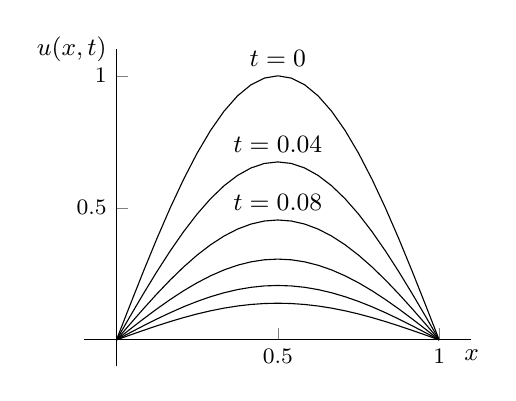
\begin{tikzpicture}
\begin{axis}[axis lines*=middle,small,xtick={0,0.5,1},xticklabels={$0$,$0.5$,$1$},ytick={0,0.5,1},yticklabels={$0$,$0.5$,$1$},xlabel={$x$},ylabel={$u(x,t)$},xlabel style={at=(current axis.right of origin)},anchor=north east,ylabel style={rotate=-90},ylabel style={at=(current axis.above origin)},anchor=north east]
\addplot[domain=0:1] {sin(180*x)*e^(-pi^2*0)}node[pos=0.5,above,font=\small]{$t=0$};
\addplot[domain=0:1] {sin(180*x)*e^(-pi^2*0.04)}node[pos=0.5,above,font=\small]{$t=0.04$};
\addplot[domain=0:1] {sin(180*x)*e^(-pi^2*0.08)}node[pos=0.5,above,font=\small]{$t=0.08$};
\addplot[domain=0:1] {sin(180*x)*e^(-pi^2*0.12)};
\addplot[domain=0:1] {sin(180*x)*e^(-pi^2*0.16)};
\addplot[domain=0:1] {sin(180*x)*e^(-pi^2*0.2)};
\end{axis}
\end{tikzpicture}
\caption{سلاخ میں حرارت (مثال \حوالہ{مثال_اعدادی_کرینک_نکلسن})}
\label{شکل_مثال_اعدادی_کرینک_نکلسن_حرارت}
\end{figure}

\موٹا{درست نتائج کے ساتھ موازنہ:} 
موجودہ مسئلے کا درست حل درج ذیل ہے (حصہ \حوالہ{حصہ_جزوی_تفرقی_بہاو_حرارت})۔
\begin{align*}
u(x,t)=\sin\pi xe^{-\pi^2 t}
\end{align*}
اعدادی نتائج کا موازنہ اب پیش کرتے ہیں۔


\موٹا{حل برائے بلا واسطہ ترکیب، مساوات \حوالہ{مساوات_اعدادی_حراری_ٹ} جہاں \عددی{r=0.25} ہے۔}\عددی{r=\tfrac{k}{h^2}=0.25} اور  \عددی{h=0.2} سے \عددی{k=rh^2=0.25\cdot 0.04=0.01} ملتا ہے لہٰذا ہمیں ترکیب کرینک نکلسن سے چار گنا زیادہ قدم چلنا ہو گا۔ \عددی{r=0.25} لیتے ہوئے مساوات \حوالہ{مساوات_اعدادی_حراری_ٹ} درج ذیل صورت اختیار کرتی ہے۔
\begin{align}\label{مساوات_اعدادی_مثال_کرینک_نکلسن}
u_{i,j+1}=0.25(u_{i-1,j}+2u_{ij}+u_{i+1,j})
\end{align}
ہم پہلے کی طرح یہاں بھی تشاکل کو استعمال کریں گے۔قدم وقت \عددی{j=1} میں ہم
\begin{align*}
u_{00}=0,\quad u_{10}=\num{0.587785}, \quad u_{20}=u_{30}=\num{0.951057}
\end{align*}
 کو استعمال کرتے ہوئے درج ذیل حاصل کرتے ہیں۔
\begin{align*}
u_{11}&=0.25(u_{00}+2u_{10}+u_{20})=\num{0.531657}\\
u_{21}&=0.25(u_{10}+2u_{20}+u_{30})=0.25(u_{10}+3u_{20})=\num{0.860239}
\end{align*}
ظاہر ہے کہ ہم سرحدی اجزاء \عددی{u_{01}=0} اور \عددی{u_{02}=0} کو کلیات سے حذف کر سکتے ہیں۔دوسری قدم وقت (\عددی{j=2}) میں درج ذیل حاصل ہو گا۔
\begin{align*}
u_{12}&=0.25(2u_{11}+u_{21})=\num{0.480888}\\
u_{22}&=0.25(u_{11}+3u_{21})=\num{0.778094}
\end{align*}
اسی طرح باقی قیمتیں حاصل کی جاتی ہیں۔ہمیں \عددی{20} قدم لینے ہوں گے لیکن درج ذیل اعدادی نتائج کے تحت درستگی تقریباً  وہی ہے جو کرینک نکلسن ترکیب سے حاصل ہوئی ہے (تین اعشاریہ تک بالکل درست قیمتیں بھی دی گئی ہیں)۔
\begin{align*}
\centering
\begin{otherlanguage}{english}
\begin{array}{C|CCC|CCC}
\hline
\multirow{2}{*}{$t$}&&x=0.2&&&x=0.4&\\
&\text{\RL{\urdufont{کرینک نکلسن}}}&\text{\RL{\urdufont{مساوات \حوالہ{مساوات_اعدادی_مثال_کرینک_نکلسن}}}}&\text{\urdufont{درست}}&\text{\RL{\urdufont{کرینک نکلسن}}}&\text{\RL{\urdufont{مساوات \حوالہ{مساوات_اعدادی_مثال_کرینک_نکلسن}}}}&\text{\urdufont{درست}}\\
\hline
0.04&0.399&0.393&0.396&0.646&0.637&0.641\\
0.08&0.271&0.263&0.267&0.439&0.426&0.432\\
0.12&0.184&0.176&0.180&0.298&0.285&0.291\\
0.16&0.125&0.118&0.121&0.202&0.191&0.196\\
0.20&0.085&0.079&0.082&0.138&0.128&0.132\\
\hline
\end{array}
\end{otherlanguage}
\end{align*}

\موٹا{مساوات \حوالہ{مساوات_اعدادی_حراری_ث} مطمئن نہ ہونے کی صورت میں مساوات \حوالہ{مساوات_اعدادی_حراری_ٹ} کی نا کامی:} \عددی{h=0.2} اور \عددی{r=1} لینے سے مساوات \حوالہ{مساوات_اعدادی_حراری_ث} مطمئن نہیں ہو گا جبکہ مساوات \حوالہ{مساوات_اعدادی_حراری_ٹ} درج ذیل صورت اختیار کرے گی
\begin{align*}
u_{i,j+1}=u_{i-1,j}-u{ij}+u_{i+1,j}
\end{align*}
جو درج ذیل نتائج دیتی ہے جو زیادہ درست نہیں ہیں۔
\begin{align*}
\centering
\begin{otherlanguage}{english}
\begin{array}{C|CC|CC}
\hline
t&x=0.2&\text{\urdufont{درست}}&x=0.4&\text{\urdufont{درست}}\\
\hline
0.04&0.363&0.396&0.588&0.641\\
0.12&0.139&0.180&0.225&0.291\\
0.20&0.053&0.082&0.086&0.132\\
\hline
\end{array}
\end{otherlanguage}
\end{align*}

\عددی{h=0.2} رکھتے ہوئے \عددی{r} کی مزید بڑی قیمت \عددی{r=2.5} لینے سے مساوات \حوالہ{مساوات_اعدادی_حراری_ٹ} بے معنی نتائج دیتی ہے۔چند نتائج درج ذیل ہیں۔
\begin{align*}
\centering
\begin{otherlanguage}{english}
\begin{array}{C|CC|CC}
\hline
t&x=0.2&\text{\urdufont{درست}}&x=0.4&\text{\urdufont{درست}}\\
\hline
0.1&0.0265&0.2191&0.0429&0.3545\\
0.3&0.0001&0.0304&0.0001&0.0492\\
0.5&0.0018&0.0042&-0.0011&0.0068\\
\hline
\end{array}
\end{otherlanguage}
\end{align*}
\انتہا{مثال}
%=============================

\حصہء{سوالات}
%=====================
\ابتدا{سوال}\شناخت{سوال_اعدادی_غیر_بعدی_معیاری_حراری_مساوات}\quad \موٹا{(غیر بعدی صورت)} \quad
\عددی{x=\tfrac{\tilde{x}}{l}}، \عددی{t=\tfrac{c^2\tilde{t}}{l^2}} اور \عددی{u=\tfrac{\tilde{u}}{u_0}} لیتے ہوئے حراری مساوات \عددی{\tilde{u}_{\tilde{t}}=c^2\tilde{u}_{\tilde{x}\tilde{x}},\,0\le \tilde{x}\le l} کا تبادل غیر بعدی معیاری صورت \عددی{u_t=u_{xx},\,\, 0\le x\le 1}  میں کریں جہاں \عددی{u_0} کوئی مستقل درجہ حرارت ہے۔
\انتہا{سوال}
%===========================
\ابتدا{سوال}\شناخت{سوال_اعدادی_کرینک_نکلسن_حراری_حل}\quad
حراری مساوات \حوالہ{مساوات_اعدادی_حراری_الف} کو مساوات \حوالہ{مساوات_اعدادی_حراری_پ} کی سرحدی شرائط اور درج ذیل ابتدائی شرائط کے لئے ترکیب کرینک نکلسن (مساوات \حوالہ{مساوات_اعدادی_کرینک_نکلسن_ب}) کی مدد سے \عددی{h=0.2}  لیتے ہوئے \عددی{0\le t\le 0.20} کے لئے حل کریں۔
\begin{align*}
f(x)=
\begin{cases}
x& 0\le x\le \tfrac{1}{2}\\
1-x&\tfrac{1}{2}< x\le 1
\end{cases}
\end{align*}
\انتہا{سوال}
%==========================
\ابتدا{سوال}\شناخت{سوال_اعدادی_نکلسن_درکار_الف}\quad
\عددی{h=0.2} اور \عددی{r=0.25} لیتے ہوئے \عددی{8} قدموں تک سوال \حوالہ{سوال_اعدادی_کرینک_نکلسن_حراری_حل} کو بلا واسطہ ترکیب سے حل کریں۔حاصل نتائج کا تین اعشاریہ درست کرینک نکلسن جوابات \عددی{0.107}، \عددی{0.175}، اور تین اعشاریہ بالکل درست جوابات \عددی{0.108}، \عددی{0.175} کے ساتھ کریں۔\\
جواب:\quad
\عددی{t=0.04} کے لئے \عددی{0.156,\,0.254} ہیں، \عددی{t=0.08} کے لئے \عددی{0.105,\,0.170} ہیں، \نقطے
\انتہا{سوال}
%==========================
\ابتدا{سوال}\quad
\عددی{x=0.2,\,0.4} اور \عددی{t=0.04,0.08,\cdots,0.20} لیتے ہوئے  مثال \حوالہ{مثال_جزوی_حراری_الف} کی تسلسل سے سوال \حوالہ{سوال_اعدادی_کرینک_نکلسن_حراری_حل} کے نتائج حاصل کریں۔
\انتہا{سوال}
%========================
\ابتدا{سوال}\quad
بلا واسطہ ترکیب کی درستگی \عددی{r\,(\le \tfrac{1}{2})} پر منحصر ہے۔سوال \حوالہ{سوال_اعدادی_نکلسن_درکار_الف} میں پہلے کی طرح \عددی{h=0.2} رکھتے ہوئے  \عددی{r=\tfrac{1}{2}} لے کر چار قدم تک حل کریں۔\عددی{t=0.04} اور \عددی{t=0.08} پر حاصل نتائج کا سوال \حوالہ{سوال_اعدادی_نکلسن_درکار_الف} کے نتائج کے ساتھ موازنہ کریں۔ \\
جواب:\quad
\عددی{x=0.2,0.4} کے لئے \عددی{t=0.04} پر \عددی{0.150,0.250} اور
 \عددی{t=0.0.08} کے لئے \عددی{0.100,0.162} ہیں۔
\انتہا{سوال}
%======================
\ابتدا{سوال}\شناخت{سوال_اعدادی_نکلسن_درکار_ب}\quad
اطراف سے حاجز شدہ متجانس سلاخ کے سر \عددی{x=0} اور  \عددی{x=1} پر ہیں۔ بائیں سر کو \عددی{\SI{0}{\celsius}} پر رکھا گیا ہے  جبکہ  دائیں سر  پر درجہ حرارت \عددی{u(t,1)=g(t)=\sin\tfrac{25}{3}\pi t} ہے۔سلاخ میں درجہ حرارت کو بلا واسطہ ترکیب سے ایک دوری عرصہ \عددی{0\le t\le 0.24} کے لئے حاصل کریں۔\عددی{h=0.2} اور \عددی{r=0.5} لیں۔(مساوات \حوالہ{مساوات_اعدادی_حراری_الف} کا حل درکار ہے۔)
\انتہا{سوال}
%=======================
\ابتدا{سوال}\شناخت{سوال_اعدادی_نکلسن_درکار_پ}\quad
سلاخ کا بایاں سر \عددی{\SI{0}{\celsius}} کی بجائے \عددی{-g(t)} پر رکھتے ہوئے  سوال \حوالہ{سوال_اعدادی_نکلسن_درکار_ب} میں \عددی{u(x,0.12)} اور \عددی{u(x,0.24)} تلاش کریں۔باقی تمام مواد وہی رکھیں۔\\
جواب:\quad
\عددی{t=0.12} پر 
$0,-0.352,-0.153,0.153,0.352,0$
ہیں جبکہ \\
\عددی{t=0.24} پر
$0,0.344,0.166,-0.166,-0.344,0$
ہیں۔
\انتہا{سوال}
%=============================
\ابتدا{سوال}\quad
سوال \حوالہ{سوال_اعدادی_نکلسن_درکار_ب} کے نتائج استعمال کرتے ہوئے سوال \حوالہ{سوال_اعدادی_نکلسن_درکار_پ} کے نتائج کس طرح حاصل کیے جا سکتے ہیں؟  سوال  \حوالہ{سوال_اعدادی_نکلسن_درکار_ب} کے نتائج 
\begin{align*}
\text{ہیں}\quad 0.054,0.172,0.325,0.406\quad \text{\RL{کے لئے}}\quad t=0.12,x=0.2,0.4,0.6,0.8\\
\text{\RL{ہیں۔}}\quad -0.009,-0.086,-0.252,-0.353\quad \text{\RL{کے لئے}}\quad t=0.24 \quad \text{اور}
\end{align*}
انہیں استعمال کرتے ہوئے سوال \حوالہ{سوال_اعدادی_نکلسن_درکار_پ} کے نتائج پرکھیں۔
\انتہا{سوال}
%=====================
\ابتدا{سوال}\شناخت{سوال_اعدادی_نکلسن_درکار_ت}\quad
اگر اطراف سے حاجز شدہ \عددی{x=0} تا \عددی{x=1} لمبی سلاخ  کا بایاں سر حاجز شدہ ہو تب \عددی{x=0} پر سرحدی شرط \عددی{u_n(0,t)=u_x(0,t)=0} ہو گا۔دکھائیں کہ مساوات \حوالہ{مساوات_اعدادی_حراری_ٹ} میں دی گئی بلا واسطہ ترکیب کی استعمال سے ہم \عددی{u_{0,j+1}} کو درج ذیل کلیہ سے حاصل کر سکتے ہیں۔ 
\begin{align*}
u_{0,j+1}=(1-2r)u_{0j}+2ru_{1j}
\end{align*}
\انتہا{سوال}
%===================
\ابتدا{سوال}\quad
ایک سلاخ جو \عددی{x=0} تا \عددی{x=1} ہے اطراف سے حاجز شدہ  ہے۔اس کا بایاں سر حاجز شدہ ہے، دائیں سر پر درجہ حرارت \عددی{g(t)=\sin\tfrac{50}{3}\pi t} ہے جبکہ \عددی{u(x,0)=0} ہے۔بلا واسطہ ترکیب میں \عددی{h=0.2} اور \عددی{r=0.25} لیتے ہوئے درجہ حرارت \عددی{u(x,t),\, 0\le t\le 0.12} تلاش کریں۔اشارہ۔  سوال \حوالہ{سوال_اعدادی_نکلسن_درکار_ت} کو دیکھیں۔
\انتہا{سوال}
%==========================

\حصہ{اعدادی تراکیب برائے قطع زائد مساوات}
اس حصہ میں ہم مساوات موج اور مطلوبہ شرائط
\begin{align}
u_{tt}&=u_{xx}\quad \quad \quad 0\le x\le 1,\, t>0\label{مساوات_اعدادی_موج_الف}\\
u(x,0)&=f(x)\quad \quad \quad \text{\RL{(ابتدائی ہٹاو)}}\label{مساوات_اعدادی_موج_ب}\\
u_t(x,0)&=g(x)\quad\quad \quad \text{\RL{(ابتدائی سمتی رفتار)}}\label{مساوات_اعدادی_موج_پ}\\
u(0,t)&=u(1,t)=0\quad\quad\quad \text{\RL{(سرحدی شرائط)}}\label{مساوات_اعدادی_موج_ت}
\end{align}
 کو مثال بناتے ہوئے  قطع زائد مساوات کے اعدادی حل پر غور کریں گے۔یاد رہے کہ \عددی{x} کے کسی بھی وقفہ اور مساوات  \عددی{u_{tt}=c^2u_{xx}} کو \عددی{x} اور \عددی{t} کے موزوں خطی تبادل سے (سوال \حوالہ{سوال_اعدادی_غیر_بعدی_معیاری_حراری_مساوات} کے تبادل کی طرح) مساوات \حوالہ{مساوات_اعدادی_موج_الف} میں تبدیل کیا جا سکتا ہے۔

ایک لچکدار ارتعاش پذیر دھاگہ جس کے سر \عددی{x=0} اور \عددی{x=1} پر باندھے گئے ہوں کا \عددی{t>0} پر حرکت کے مسئلہ  کو مساوات \حوالہ{مساوات_اعدادی_موج_الف} تا مساوات \حوالہ{مساوات_اعدادی_موج_ت} پیش کرتے ہیں۔اس مسئلے کا حل مساوات \حوالہ{مساوات_جزوی_موج_مساوات_ج} میں دیا گیا ہے۔

مساوات میں پہلے کی طرح تفرق کی جگہ فرق کے حاصل تقسیم پر کرتے ہیں۔یوں مساوات \حوالہ{مساوات_اعدادی_موج_الف} سے 
\begin{align}\label{مساوات_اعدادی_موج_ٹ}
\frac{1}{k^2}[u_{i,j+1}-2u_{ij}+u_{i,j-1}]=\frac{1}{h^2}[u_{i+1,j}-2u_{ij}+u_{i-1,j}]
\end{align}
حاصل ہو گا جہاں \عددی{x} رخ جسامت جال \عددی{h} اور \عددی{t} رخ جسامت جال \عددی{k} ہے۔درج بالا مساوات فرق شکل \حوالہ{مساوات_اعدادی_مساوات_موج_الف}-الف میں دکھائے گئے پانچ نقطوں کا آپس میں تعلق بیان کرتی ہے۔اس سے ہم کہہ سکتے ہیں کہ، گزشتہ حصے کی قطع مکافی مساوات کی طرح،  ہمیں یہاں بھی مستطیل جال درکار ہو گا۔ہم \عددی{r^*=\tfrac{k^2}{h^2}=1} لیتے ہیں جس سے  \عددی{u_{ij}} حذف ہو گا (شکل \حوالہ{مساوات_اعدادی_مساوات_موج_الف}-ب)  اور مساوات \حوالہ{مساوات_اعدادی_موج_ٹ} درج ذیل صورت اختیار کرے گی۔
\begin{align}\label{مساوات_اعدادی_موج_ث}
u_{i,j+1}=u_{i-1,j}+u_{i+1,j}-u_{i,j-1}
\end{align}
%
\begin{figure}
\centering
\begin{subfigure}{0.3\textwidth}
\centering
\begin{tikzpicture}
\draw(-1,0)--(1,0);
\draw(0,-1)--(0,1);
\fill[white](-1,0) circle (1.5pt)  (0,0) circle (1.5pt) (1,0) circle (1.5pt)  (0,-1) circle (1.5pt)  (0,1) circle (1.5pt); 
\draw (-1,0)node[kcross]{}   (0,0)node[kcross]{} (1,0)node[kcross]{} (0,-1)node[kcross]{} (0,1)node[kcross]{};
\draw (-0.5,0)node[below]{$h$}  (0.5,0)node[below]{$h$} (0,-0.5)node[right]{$k$}  (0,0.5)node[right]{$k$};
\end{tikzpicture}
\caption*{(الف) مساوات \حوالہ{مساوات_اعدادی_موج_ٹ}}
\end{subfigure}%
\begin{subfigure}{0.3\textwidth}
\centering
\begin{tikzpicture}
\draw(0,1)node[]{\RL{صف وقت \عددی{j+1}}};
\draw(0,0)node[]{\RL{صف وقت \عددی{j}}};
\draw(0,-1)node[]{\RL{صف وقت \عددی{j-1}}};
\end{tikzpicture}
\end{subfigure}%
\begin{subfigure}{0.3\textwidth}
\centering
\begin{tikzpicture}
\draw(-1,0)--(1,0);
\draw(0,-1)--(0,1);
\fill[white](-1,0) circle (1.5pt)  (0,0) circle (1.5pt) (1,0) circle (1.5pt)  (0,-1) circle (1.5pt)  (0,1) circle (2.5pt); 
\draw (-1,0)node[kcross]{}  (1,0)node[kcross]{} (0,-1)node[kcross]{} (0,1)node[circ]{};
\end{tikzpicture}
\caption*{(ب) مساوات \حوالہ{مساوات_اعدادی_موج_ث}}
\end{subfigure}%
\caption{مساوات \حوالہ{مساوات_اعدادی_موج_ٹ} اور مساوات \حوالہ{مساوات_اعدادی_موج_ث} میں استعمال ہونے والے جوڑ}
\label{مساوات_اعدادی_مساوات_موج_الف}
\end{figure}
یہ ثابت کیا جا سکتا ہے کہ \عددی{0<r^*\le 1} کے لئے موجودہ ترکیب مستحکم ہے لہٰذا موجودہ ابتدائی قیمتیں جن میں عدم استمرار نہیں پایا جاتا ہے کہ لئے ہم مساوات \حوالہ{مساوات_اعدادی_موج_ث} سے  قابل توقع نتائج کی توقع رکھتے ہیں۔ (ابتدائی معلومات میں عدم استمرار کی صورت میں قطع زائد مساوات کو موجودہ طریقہ سے حل کرنے میں دشواری پیش آئے گی۔)

مساوات \حوالہ{مساوات_اعدادی_موج_ث} میں اب بھی تین قدم وقت \عددی{j-1}، \عددی{j}، \عددی{j+1} پائے جاتے ہیں جبکہ قطع مکافی کی صورت میں دو قدم وقت پائے جاتے تھے۔مزید اب دو عدد ابتدائی شرائط ہیں۔اس لئے ہم جاننا چاہیں گے کہ ہم قدم لینا کس طرح شروع کریں گے  اور مساوات \حوالہ{مساوات_اعدادی_موج_پ} میں دی گئی ابتدائی معلومات کو کس طرح استعمال کریں گے۔ان معاملات پر اب غور کرتے ہیں۔\عددی{u_t(x,0)=g(x)} سے ہم مساوات فرق
\begin{align}\label{مساوات_اعدادی_موج_ج}
\frac{1}{2k}(u_{i1}-u_{i,-1})=g_i \quad \implies \quad u_{i,-1}=u_{i1}-2kg_i
\end{align}
حاصل کرتے ہیں جہاں \عددی{g_i=g(ih)} ہے۔اب \عددی{t=0} یعنی \عددی{j=0} کے لئے مساوات \حوالہ{مساوات_اعدادی_موج_ث} درج ذیل دے گی
\begin{align*}
u_{i1}=u_{i-1,0}+u_{i+1,0}-u_{i,-1}
\end{align*}
جس میں ہم مساوات \حوالہ{مساوات_اعدادی_موج_ج} پر کرتے ہوئے \عددی{u_{i1}} کے لئے حل کر کے
\begin{align}\label{مساوات_اعدادی_موج_چ}
u_{i1}=\frac{1}{2}(u_{i-1,0}+u_{i+1,0}+kg_i)
\end{align}
حاصل کرتے ہیں جو \عددی{u_{i1}} کو ابتدائی معلومات کی صورت میں پیش کرتی ہے۔

%=====================
\ابتدا{مثال}\quad \موٹا{ارتعاش پذیر دھاگہ}\\
\عددی{h=k=0.2} لیتے ہوئے موجودہ ترکیب کی  مدد سے مساوات \حوالہ{مساوات_اعدادی_موج_الف} تا مساوات \حوالہ{مساوات_اعدادی_موج_ت} میں دیا گیا مسئلہ حل کریں جہاں \عددی{f(x)=\sin \pi x} اور \عددی{g(x)=0} ہیں۔ 

حل:\quad
ہم شکل \حوالہ{شکل_مثال_اعدادی_کرینک_نکلسن} کی جال استعمال کرتے ہیں پس \عددی{t} کی قیمتیں \عددی{0.04,0.08,\cdots} کی بجائے اب \عددی{0.2,0.4,\cdots} ہوں گی۔ابتدائی قیمتیں \عددی{u_{00},u_{10},\cdots} وہی ہوں گی جو مثال \حوالہ{مثال_اعدادی_کرینک_نکلسن} میں تھیں۔مساوات \حوالہ{مساوات_اعدادی_موج_چ} اور \عددی{g(x)=0} سے
\begin{align*}
u_{i1}=\frac{1}{2}(u_{i-1,0}+u_{i+1,0})
\end{align*}
حاصل ہو گا جس سے ہم درج ذیل حاصل کرتے ہیں۔
\begin{align*}
u_{11}&=\frac{1}{2}(u_{00}+u_{20})=\tfrac{1}{2}\cdot \num{0.951057}=\num{0.475528}\\
u_{21}&=\frac{1}{2}(u_{10}+u_{30})=\tfrac{1}{2}\cdot \num{1.538842}=\num{0.769421}
\end{align*}
یہاں بھی تشاکل کی بنا \عددی{u_{31}=u_{21}} اور \عددی{u_{41}=u_{11}} ہوں گے۔\عددی{u_{01}=u_{02}=\cdots=0} استعمال کرتے ہوئے \عددی{j=1} کے لئے مساوات \حوالہ{مساوات_اعدادی_موج_ج} سے
\begin{align*}
u_{12}&=u_{01}+u_{21}-u_{10}=\num{0.769421}-\num{0.587785}=\num{0.181636}\\
u_{22}&=u_{11}+u_{31}-u_{20}=\num{0.475528}-\num{0.769421}-\num{0.951057}=\num{0.293892}
\end{align*}
حاصل ہوں گے اور تشاکل کی بنا \عددی{u_{32}=u_{22}} اور \عددی{u_{42}=u_{12}} ہوں گے۔اسی طرح باقی قیمتیں بھی حاصل کی جاتی ہیں۔یوں دھاگے کی پہلی نصف ارتعاش کے لئے ہٹاو \عددی{u(x,t)} کی درج ذیل قیمتیں حاصل ہوں گی۔
\begin{align*}
\centering
\begin{otherlanguage}{english}
\begin{array}{CCRRRRC}
t&x=0&x=0.2&x=0.4&x=0.6&x=0.8&x=1\\
\hline
0.0&0&0.588&0.951&0.951&0.588&0\\
0.2&0&0.476&0.769&0.769&0.476&0\\
0.4&0&0.182&0.294&0.294&0.182&0\\
0.6&0&-0.182&-0.294&-0.294&-0.182&0\\
0.8&0&-0.476&-0.769&-0.769&-0.476&0\\
1.0&0&-0.588&-0.951&-0.951&-0.588&0
\end{array}
\end{otherlanguage}
\end{align*}
یہ قیمتیں بالکل درست ہیں۔اس مسئلے کا درست حل درج ذیل ہے (حصہ \حوالہ{حصہ_جزوی_علیحدگی_متغیرات})۔
\begin{align*}
u(x,t)=\sin\pi x \cos \pi t
\end{align*} 
حصہ \حوالہ{حصہ_جزوی_دا_لومبیغ_حل} میں مسئلہ دا لومبیغ کے حل کی بنا یہاں بالکل درست نتائج حاصل ہوئے ہیں (سوال \حوالہ{سوال_اعدادی_درکار_اوپر})۔
\انتہا{مثال}
%===========================

\حصہء{سوالات}
%=================
\ابتدا{سوال}\quad
ارتعاش پذیر دھاگے کے مسئلہ (مساوات \حوالہ{مساوات_اعدادی_موج_الف} تا مساوات \حوالہ{مساوات_اعدادی_موج_ت}) کو \عددی{h=k=0.2} لیتے ہوئے \عددی{0\le t\le 2} کے لئے موجودہ اعدادی ترکیب سے حل کریں۔ابتدائی انحراف \عددی{f(x)=x(1-x)}جبکہ ابتدائی رفتار صفر ہے۔\\
جواب:\quad
\عددی{x=0.2,0.4} کے لئے \عددی{(t=0.2)} پر \عددی{0.12,0.2}، \عددی{(t=0.4)} پر \عددی{0.04,0.08}، \عددی{(t=0.6)} پر \عددی{-0.04,-0.08}، وغیرہ۔
\انتہا{سوال}
%========================
\ابتدا{سوال}\شناخت{سوال_اعدادی_درکار_اوپر}\quad
دکھائیں کہ \عددی{c=1} لیتے ہوئے  مسئلہ دا لومبیغ  کے حل، مساوات \حوالہ{مساوات_جزوی_موج_مساوات_ث}، کی بنا مساوات \حوالہ{مساوات_اعدادی_موج_ث} بالکل درست حل \عددی{u_{i,j+1}=u({ih,(j+1)h})} دے گی۔
\انتہا{سوال}
%======================
\ابتدا{سوال}\شناخت{سوال_اعدادی_موج_درکار_الف}\quad
ابتدائی رفتار \عددی{g(x)=\sin \pi x} اور ابتدائی انحراف صفر  لیتے ہوئے مساوات \حوالہ{مساوات_اعدادی_موج_الف} کا حل \عددی{t=0.4} اور \عددی{x=0.2,0.4,0.6,0.8} کے لئے حاصل کریں۔موجودہ ترکیب استعمال کریں جس میں \عددی{h=0.2} اور \عددی{k=0.2} لیں۔ مساوات \حوالہ{مساوات_جزوی_موج_مساوات_ج} میں دیے گئے بالکل درست حل کے ساتھ موازنہ کریں۔\\
جواب:\quad
$0.190,0.308,0.308,0.190$ 
جبکہ تین اعشاریہ درست نتائج 
$0.178,0.288,0.288,0.178$
ہیں۔
\انتہا{سوال}
%=========================
\ابتدا{سوال}\quad
زیادہ باریک جال (\عددی{h=0.1}، \عددی{k=0.1}) لیتے ہوئے سوال \حوالہ{سوال_اعدادی_موج_درکار_الف} دوبارہ حل کریں۔مساوات \حوالہ{مساوات_جزوی_موج_مساوات_ج} میں دیے گئے بالکل درست حل کے ساتھ موازنہ کریں۔
\انتہا{سوال}
%============================
\ابتدا{سوال}\شناخت{سوال_اعدادی_درکار_موج_ب}\quad
موجودہ ترکیب کی ابتدا کا طریقہ کار اس صورت پیش کریں جب \عددی{f} اور \عددی{g} دونوں مماثلی صفر نہ ہوں مثلاً
\begin{align*}
f(x)=1-\cos 2\pi x,\quad g(x)=x-x^2;
\end{align*} 
\عددی{h=k=0.1} لیں اور دو قدم وقت تک چلیں۔\\
جواب:\quad
\عددی{t=0.1} کے لئے
$0,0.354,0.766,1.271,1.679,1.834,\cdots$\\
جبکہ \عددی{t=0.2} کے لئے
$0,0.575,0.935,1.135,1.296,1.357,\cdots$ 
\انتہا{سوال}
%========================
\ابتدا{سوال}\شناخت{سوال_اعدادی_درکار_موج_پ}\quad
دکھائیں کہ مساوات \حوالہ{مساوات_جزوی_موج_مساوات_ج} سے درج ذیل ابتدا کرنے کا کلیہ بھی دیتی ہے
\begin{align*}
u_{i1}=\tfrac{1}{2}(u_{i+1,0}+u_{i-1,0})+\tfrac{1}{2}\int_{x_i-k}^{x_i+k}g(s)\dif s
\end{align*}
(جہاں تکمل کو اعدادی تراکیب سے بھی حاصل کیا جا سکتا ہے)۔ کس صورت یہ کلیہ اور مساوات \حوالہ{مساوات_اعدادی_موج_چ} یکساں ہوں گے؟
\انتہا{سوال}
%==========================
\ابتدا{سوال}\quad
سوال \حوالہ{سوال_اعدادی_درکار_موج_پ} میں دیا گیا کلیہ استعمال کرتے ہوئے سوال \حوالہ{سوال_اعدادی_درکار_موج_ب} کو  \عددی{t=0.1} اور \عددی{x=0.1,0.2,\cdots} کے لئے حل کریں۔ نتائج کا موازنہ کریں۔
\انتہا{سوال}
%====================
\ابتدا{سوال}\quad
درج ذیل ابتدائی معلومات کے لئے مساوات \حوالہ{مساوات_اعدادی_موج_الف} حل کریں۔
\begin{align*}
u(x,0)=x^2,\quad u_t(x,0)=2x,\quad u_x(0,t)=2t,\quad u(1,t)=(1+t)^2
\end{align*}
\عددی{h=k=0.2} لیں (پانچ قدم وقت)۔

\انتہا{سوال}
%===========================
